%
The primary impetus for employing neural network reweighting, as opposed to the reweighting approach utilized in the SM-4top analysis, lies in its capacity to cover a broader range of dimensions for reweighting. 
This is attributable to the fact that in graph neural network (GNN) methodologies, such as the multivariate analysis (MVA) strategy, a greater number of fundamental variables, in conjunction with high-level variables, are employed.
In order to ensure the continued validity of this method in comparison to the previous approach, a dedicated study has been conducted, which rigorously compares both methodologies.
Initially, Figure~\ref{fig:seq_vs_nn} provides a comparative analysis of both techniques, highlighting the advantageous aspects of neural network reweighting, particularly in relation to the examination of the transverse momentum of the second leading jet.

Subsequent to the confirmation that neural network reweighting is comparably effective as the previous approach, an Asimov fit was conducted to compare both methodologies, as depicted in Figure~\ref{fig:asimov_fit_seq_nn}. 
While there were initially significant constraints imposed upon the acceptance nuisance parameters for the \ttbin\ PS selection, these constraints are no longer relevant in the most recent configuration. 
Consequently, any minor reduction in significance, as a result of these constraints, is deemed negligible. 
In conclusion, the significance of the SM-4top signal has been determined to be 1.04 using the previous method, and 0.96 when employing neural network reweighting.


\begin{figure}[htbp!]
    \begin{center} \setlength{\tabcolsep}{2.5pt}\footnotesize
    \begin{tabular}{cc}
    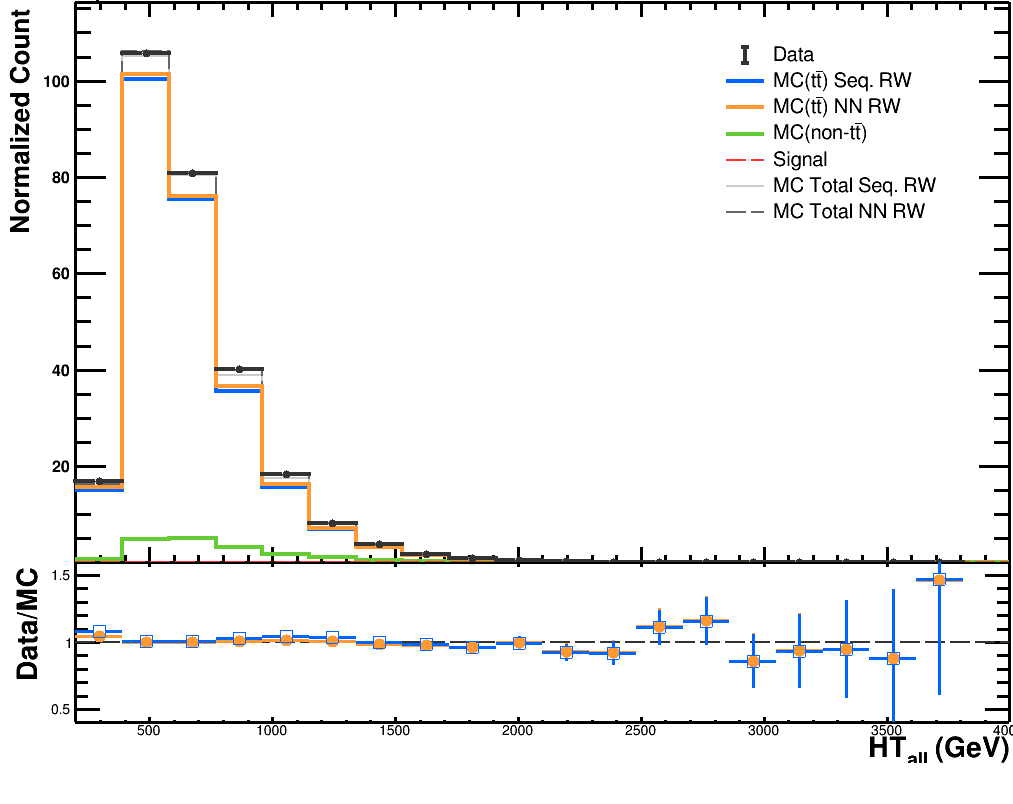
\includegraphics[width=0.46 \textwidth]{figures/background_modeling_seq_vs_nn/ratio_plotHT_all_1e3_nJets__7__nBTags_MV2c10_70__2.png} &
    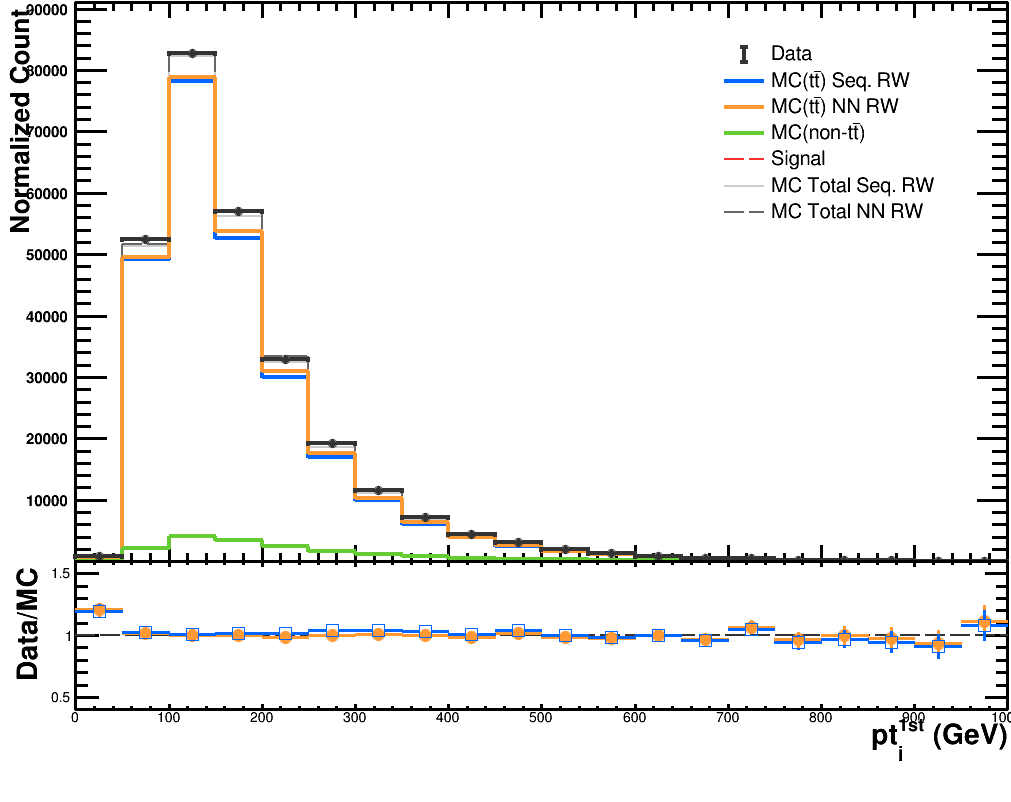
\includegraphics[width=0.46 \textwidth]{figures/background_modeling_seq_vs_nn/ratio_plotjet_pt_0__1e3_nJetsge7__nBTags_MV2c10_70ee2_NN_3Dmeff_5Ltanh_80ep_node30.png} \\

    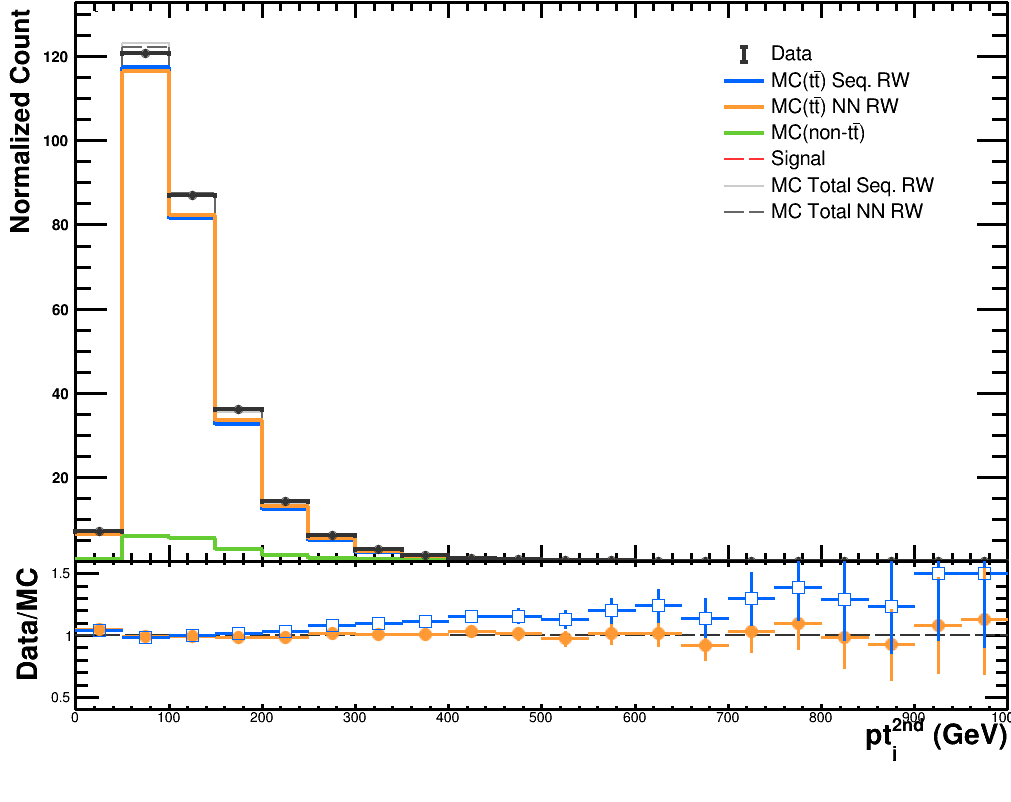
\includegraphics[width=0.46 \textwidth]{figures/background_modeling_seq_vs_nn/ratio_plotjet_pt_1__1e3_nJetsge7__nBTags_MV2c10_70ee2_NN_score_14D_5Ltanh_120ep_node30_2b.png} &
    \includegraphics[width=0.46 \textwidth]{figures/background_modeling_seq_vs_nn/ratio_plotSum__jet_pcb_MV2c10_btag_ordered__Iteration__6___nJetsee7__nBTags_MV2c10_70ee2_NN_score_16D_5Ltanh_200ep_node30_fullstat_7jin2bex_7jex3bin0J.png} \\

    \end{tabular}
    \caption{\label{fig:seq_vs_nn}The reweighting comparison from the SM-4top study (Seq. RW) vs neural network reweighting (NN. RW), for the 7 jets, and at least 2b jets region}
    
\end{center}
\end{figure}

\begin{figure}[htbp!]
    \begin{center} \setlength{\tabcolsep}{2.5pt}\footnotesize
    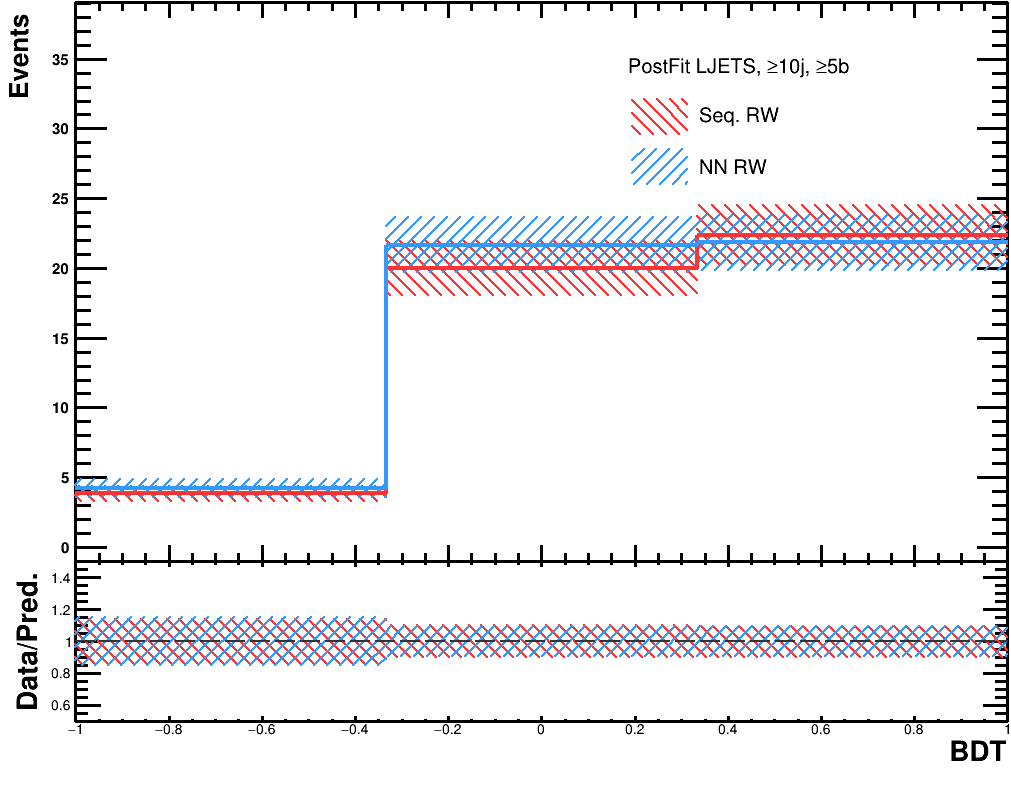
\includegraphics[width=0.76 \textwidth]{figures/background_modeling_seq_vs_nn/unc_comp.png} \\
    \begin{tabular}{cc}
    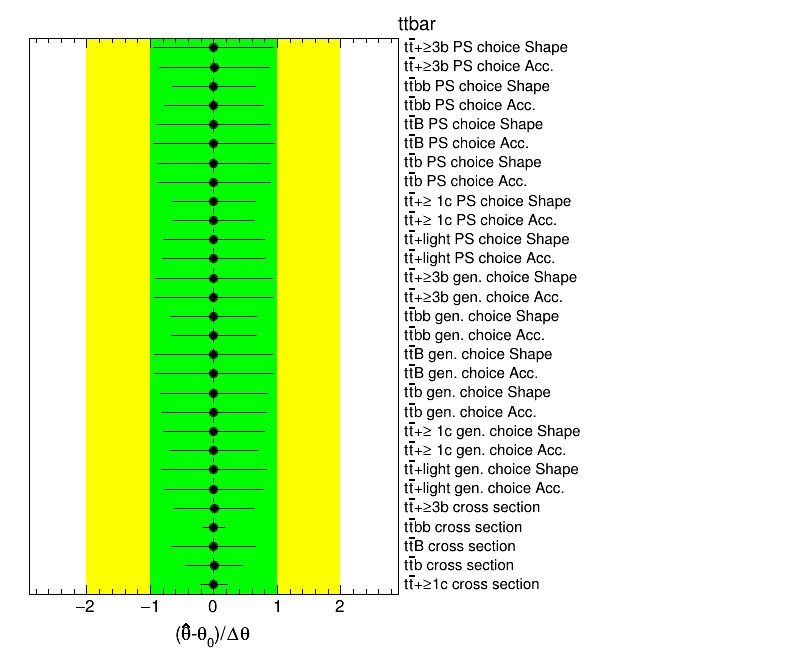
\includegraphics[width=0.46 \textwidth]{figures/background_modeling_seq_vs_nn/syst_seq.png} &
    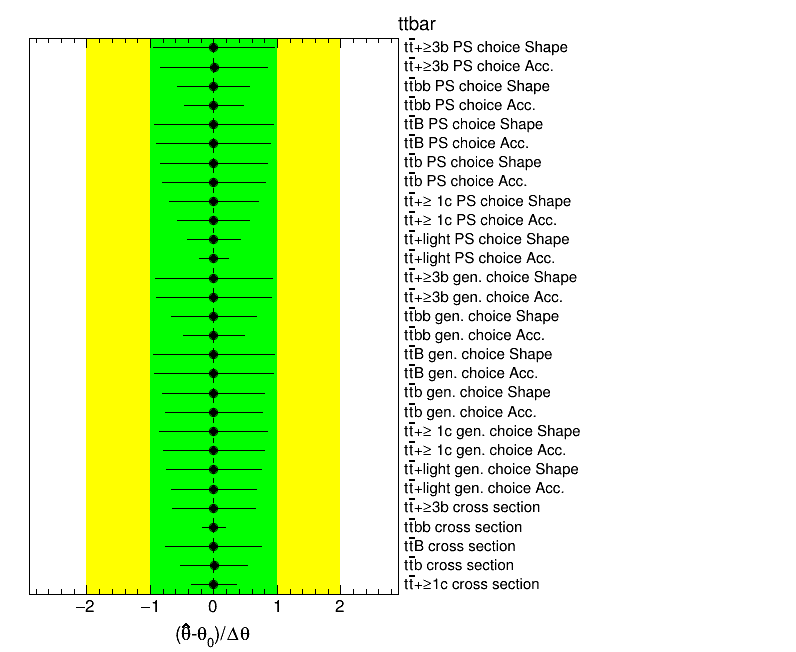
\includegraphics[width=0.46 \textwidth]{figures/background_modeling_seq_vs_nn/syst_nn.png} \\
    \end{tabular}
    \caption{\label{fig:asimov_fit_seq_nn} (Top) The post-fit uncertainty comparison between Seq. RW and NN. RW use cases, (bottom-left) nuisance parameters fit in the case of Seq. RW uses, and (bottom-right) in the case of NN. RW usage.}    
\end{center}
\end{figure}

Comparison of NN reweighting and the reweighting used for SM 4top study can be found at \url{https://asonay.web.cern.ch/asonay/bsm4top/datamc_ljets.html} and \url{https://asonay.web.cern.ch/asonay/bsm4top/datamc_os2l.html} for 1L and 2LOS respectively.
These plots are produced by old samples using EMTopo jets due to being identical with SM 4top study. 
Later comprehensive comparison studied with PFlow jets in \url{https://asonay.web.cern.ch/asonay/bsm4top/datamc_ljets_pflow.html}
More recent study can be found in Figure~\ref{fig:recent_rew_1los} and Figure~\ref{fig:recent_rew_2los}.
Also some other NN reweighting plots are illustrated in Appendix~\ref{app:NNRewPlots}

\begin{figure}[htbp!]
    \begin{center} \setlength{\tabcolsep}{2.5pt}\footnotesize
    \begin{tabular}{cccc}
    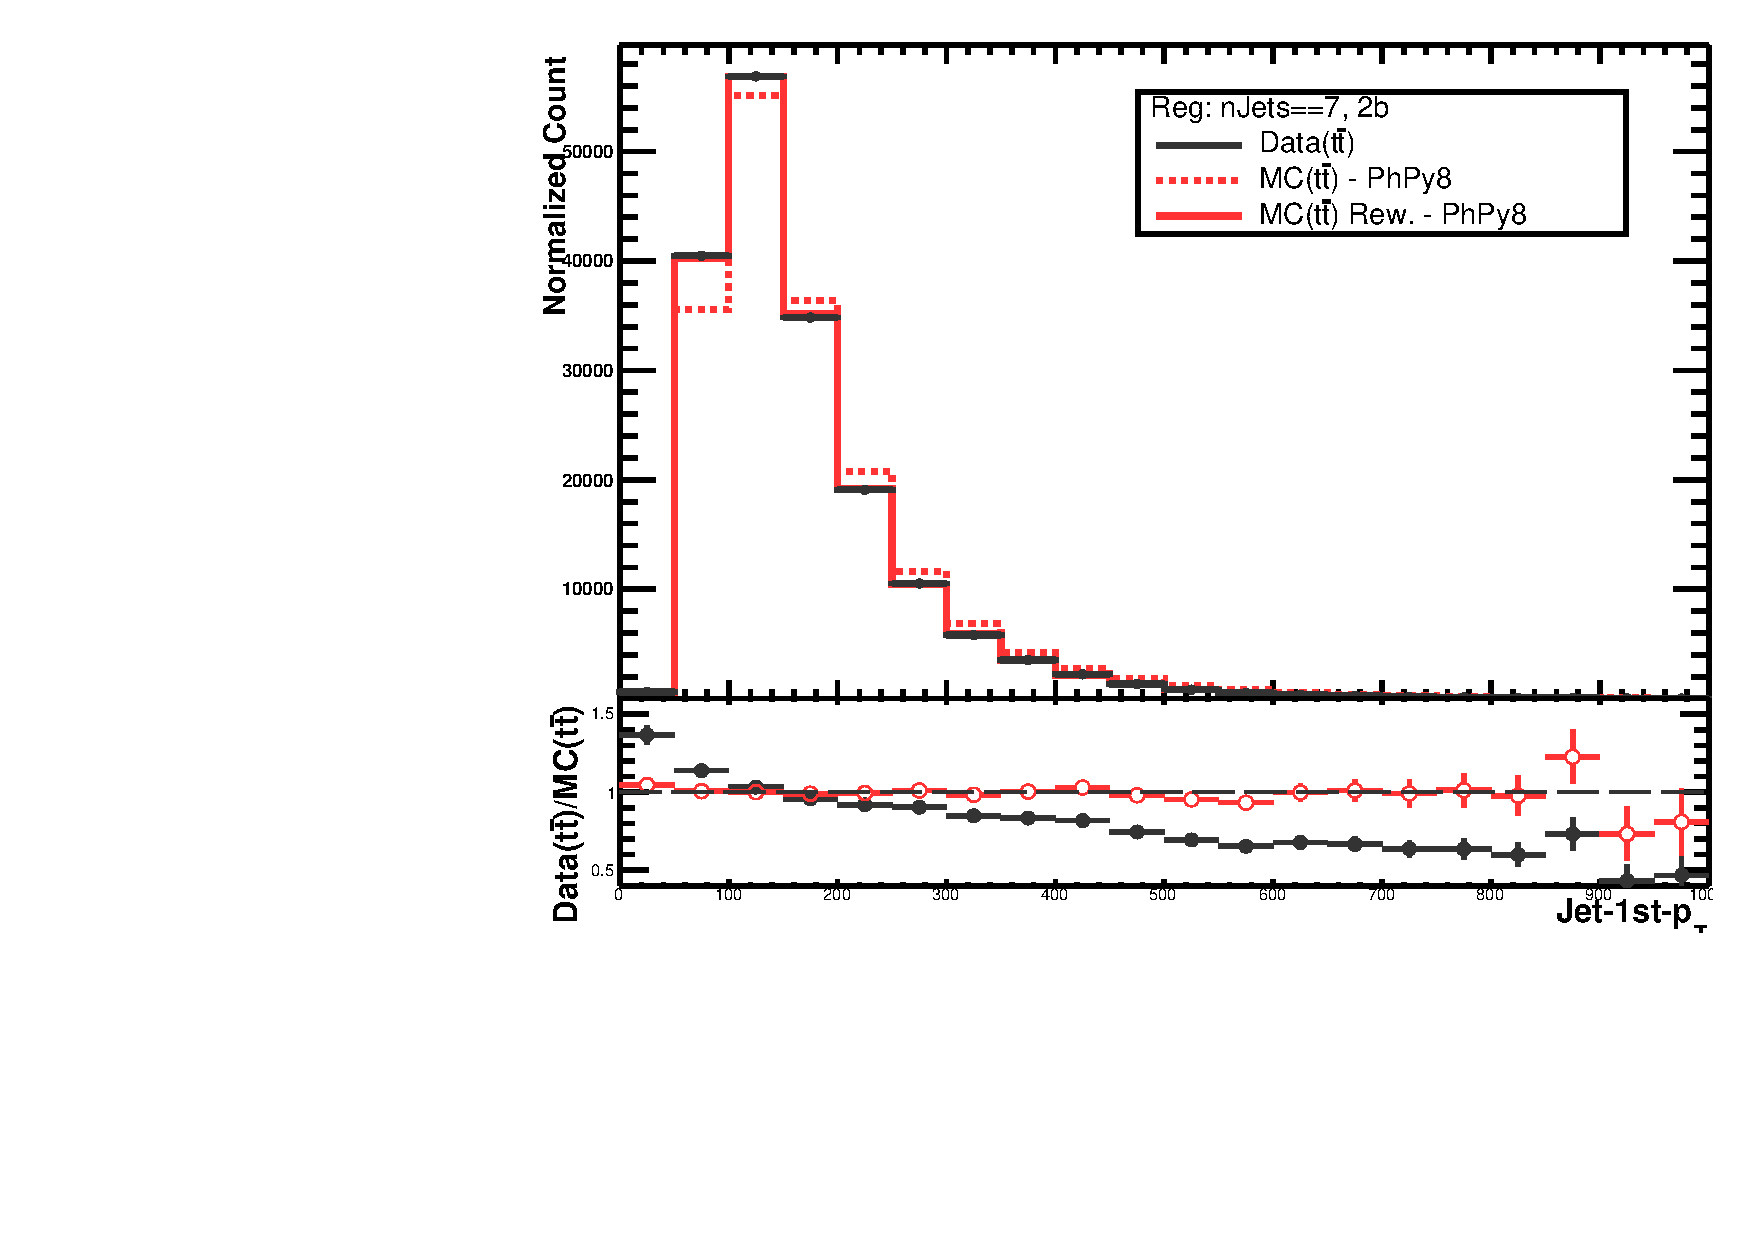
\includegraphics[width=0.24 \textwidth]{figures/rew_datamc_hfinckin_212169/1_ratiojet_pt_0__1e3_nJetsee7__1LOS.pdf} &
    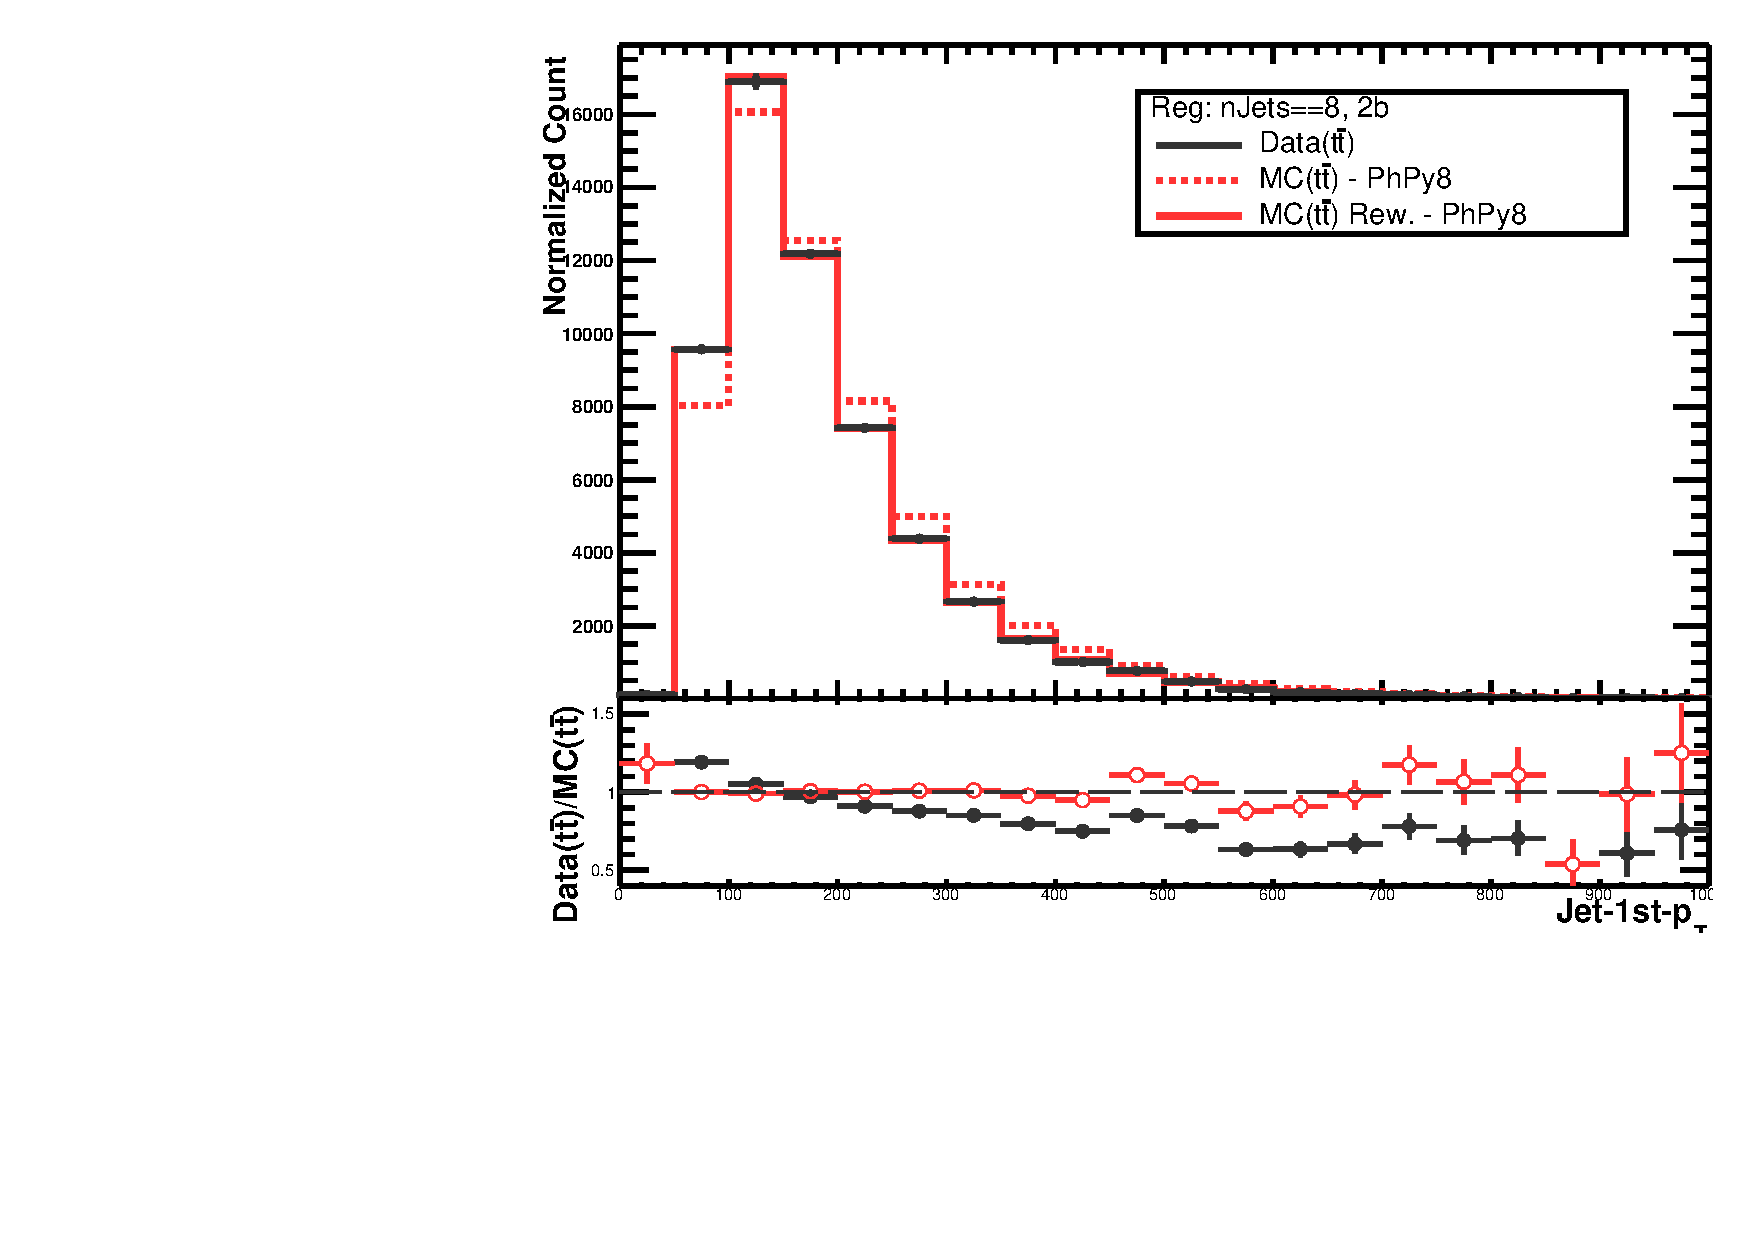
\includegraphics[width=0.24 \textwidth]{figures/rew_datamc_hfinckin_212169/1_ratiojet_pt_0__1e3_nJetsee8__1LOS.pdf} &
    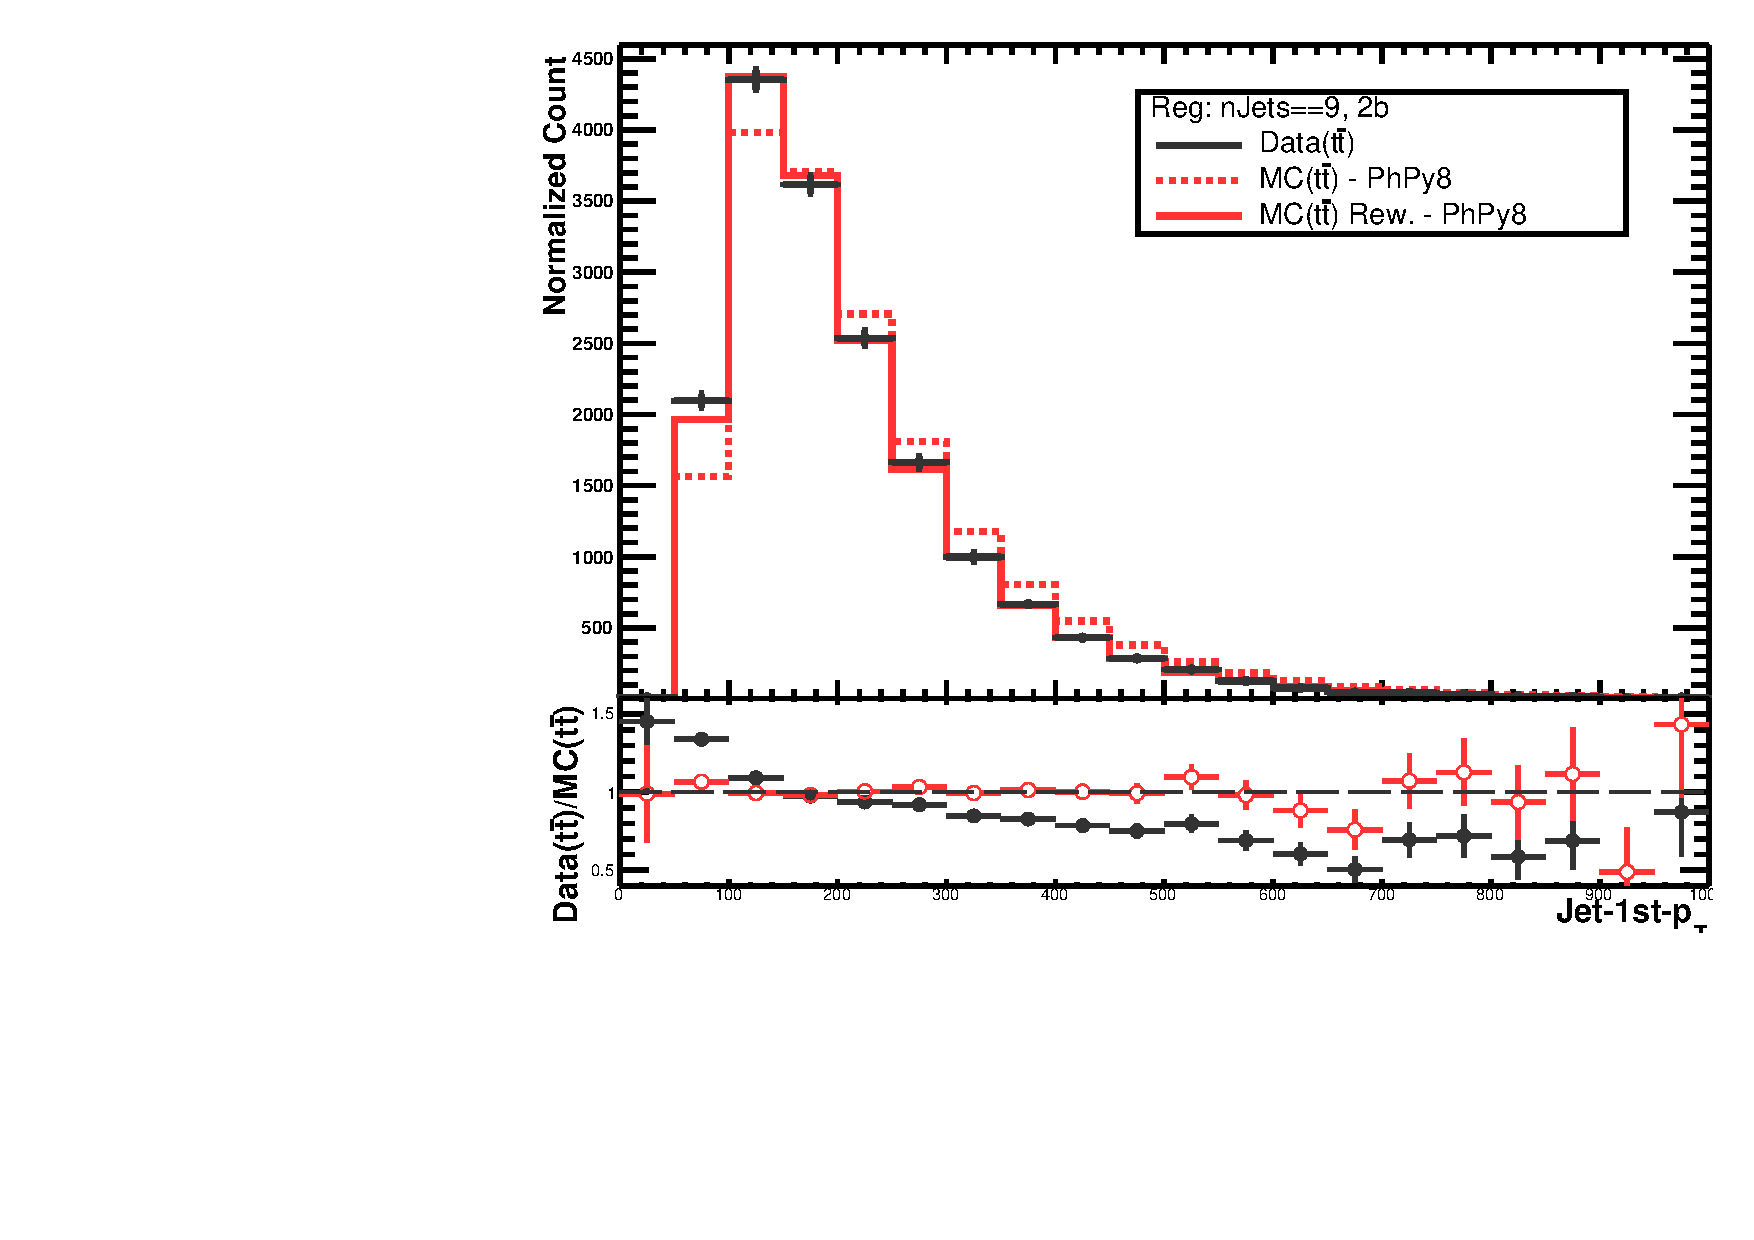
\includegraphics[width=0.24 \textwidth]{figures/rew_datamc_hfinckin_212169/1_ratiojet_pt_0__1e3_nJetsee9__1LOS.pdf} &
    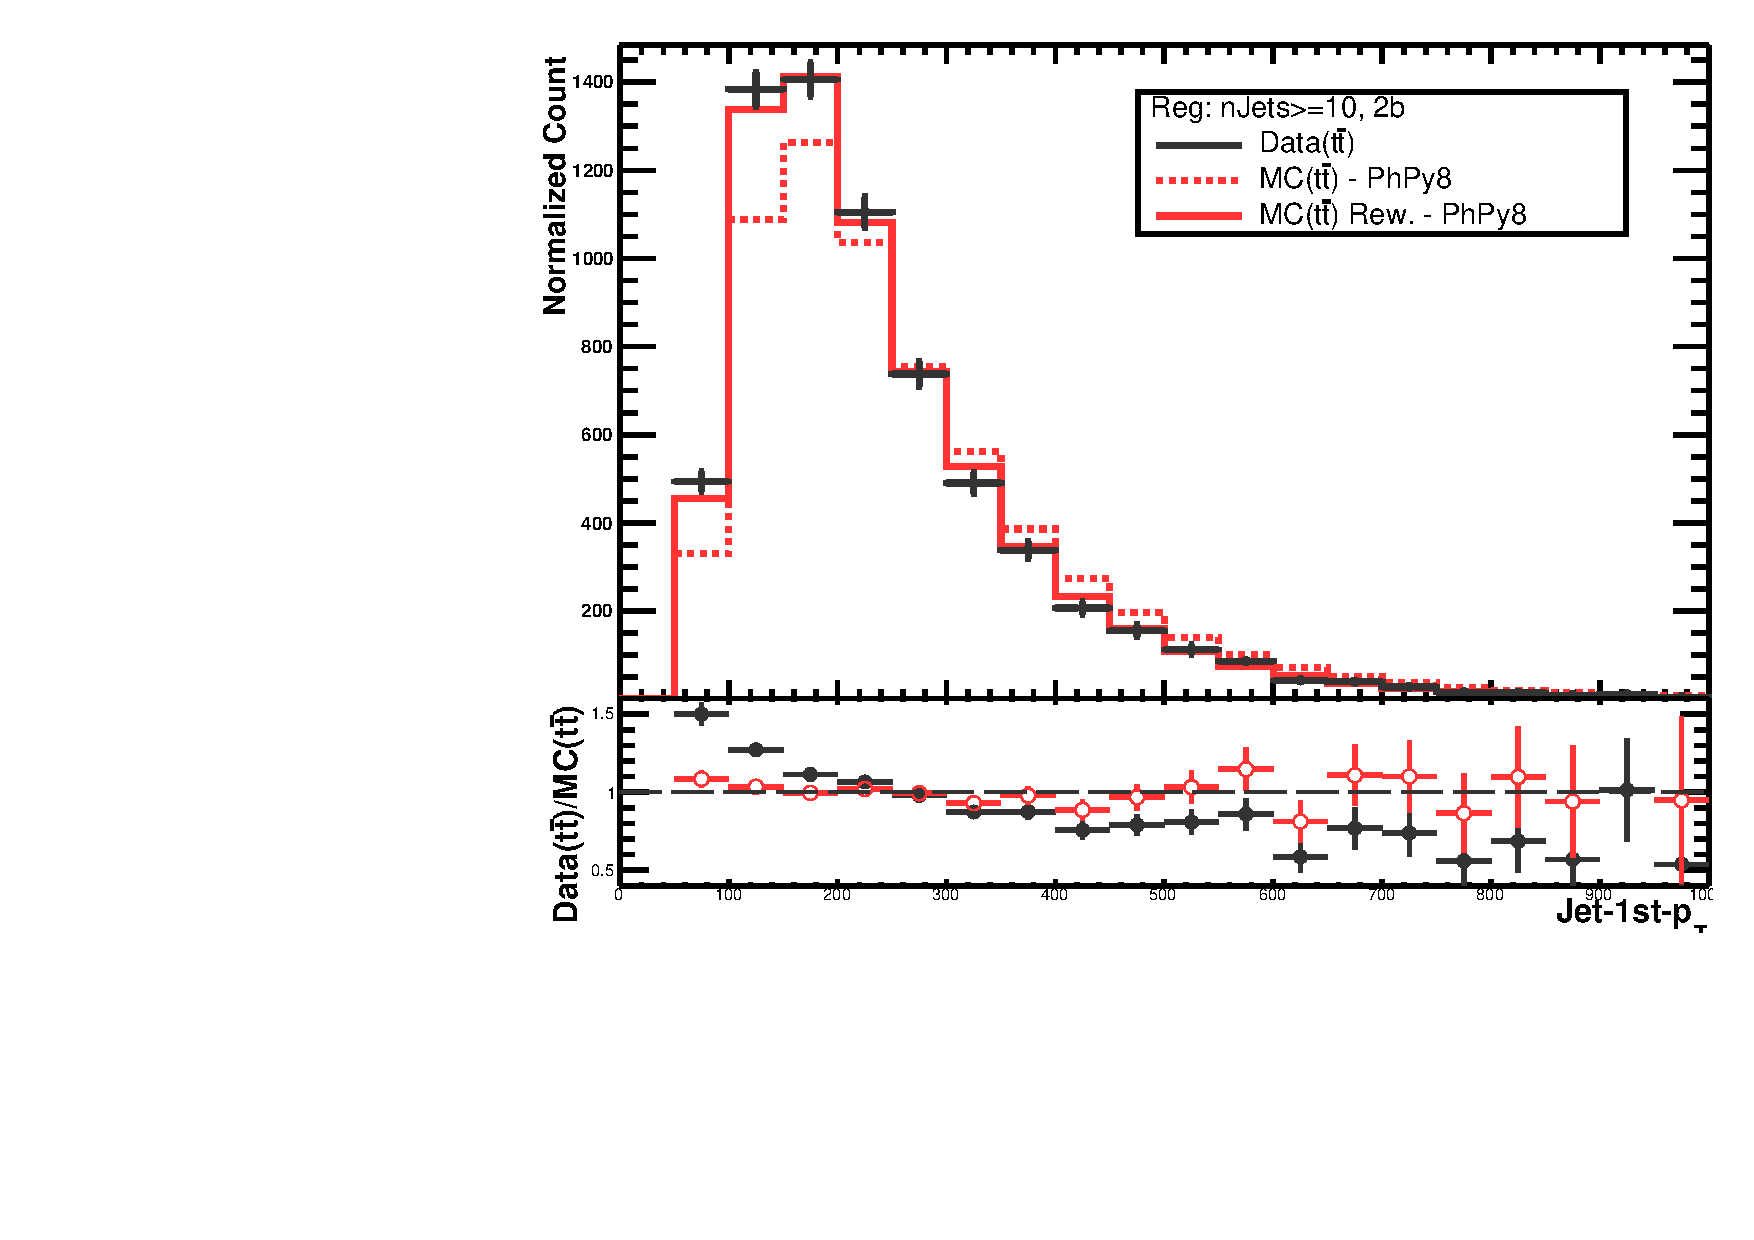
\includegraphics[width=0.24 \textwidth]{figures/rew_datamc_hfinckin_212169/1_ratiojet_pt_0__1e3_nJetsge10__1LOS.pdf} \\

    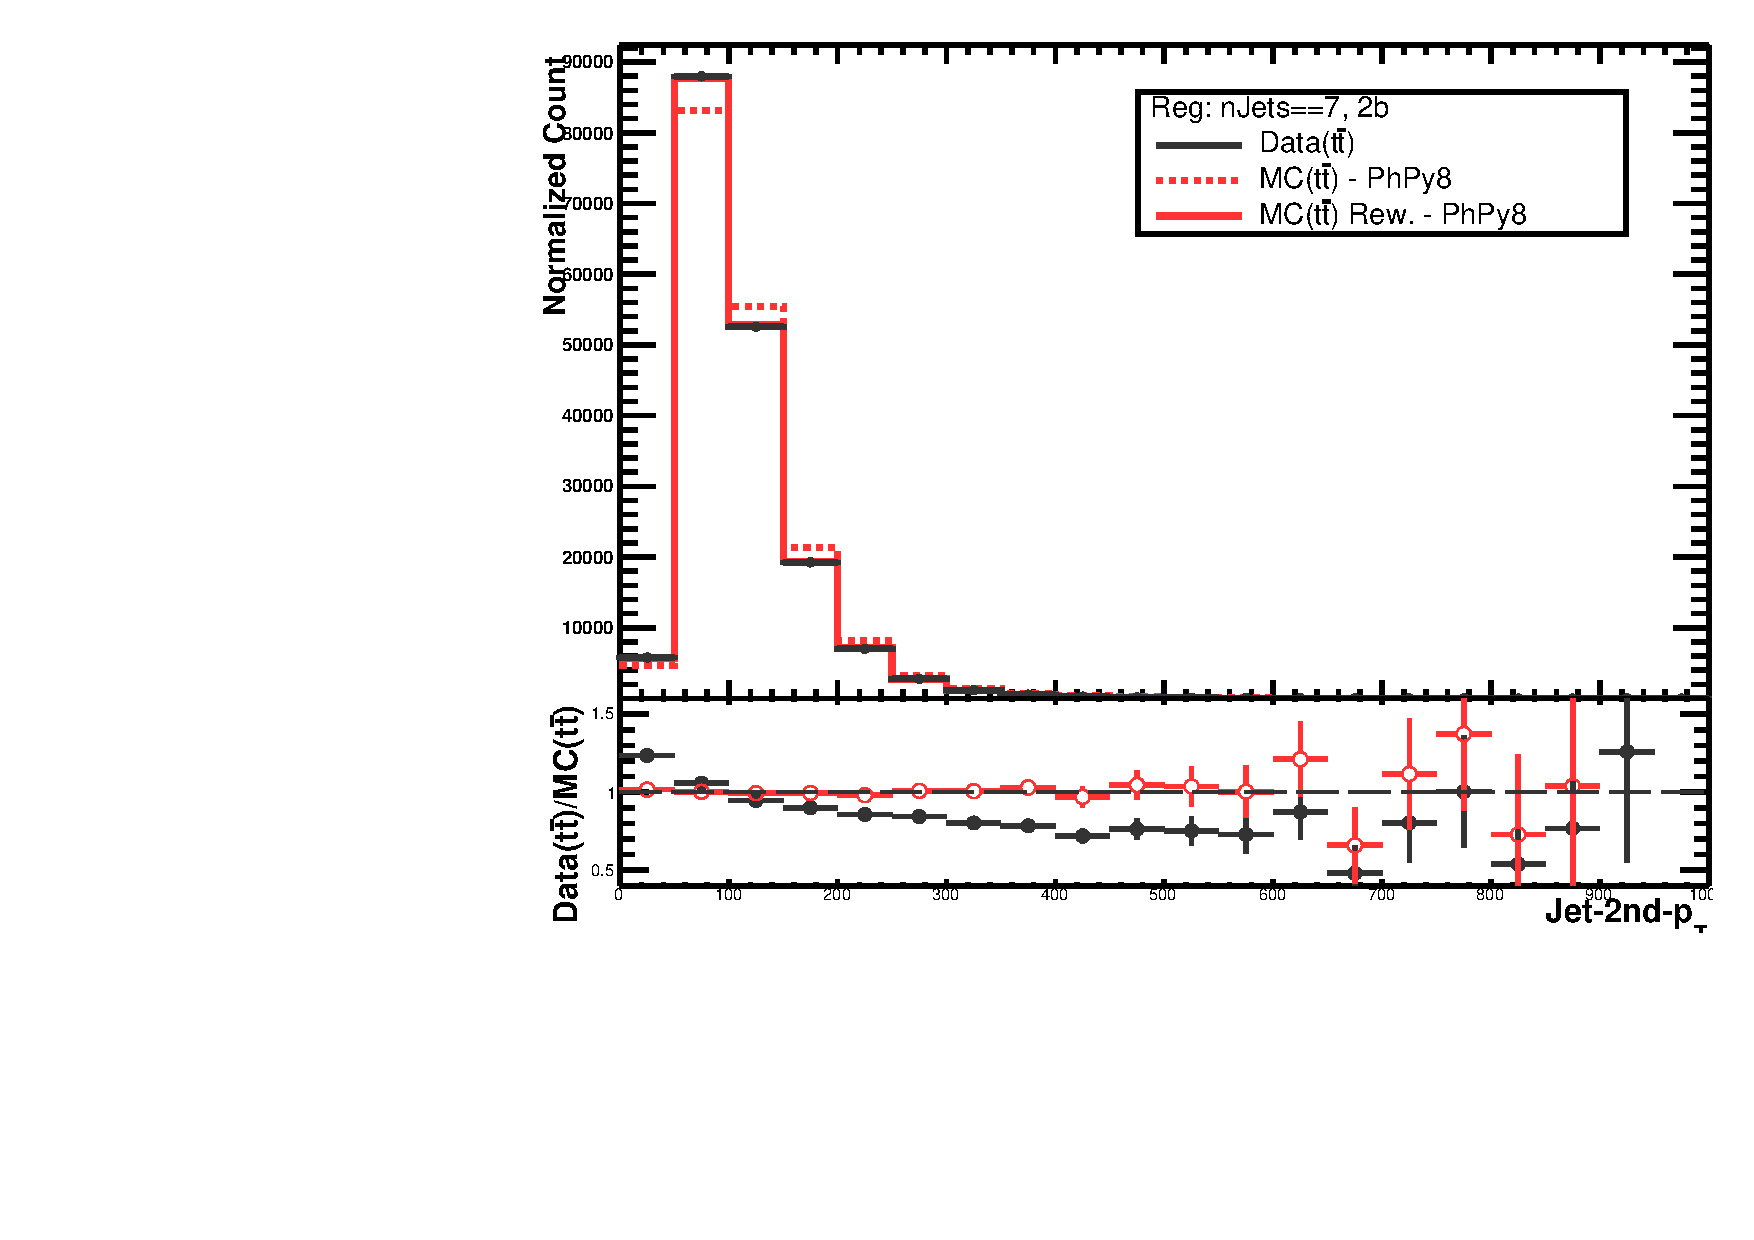
\includegraphics[width=0.24 \textwidth]{figures/rew_datamc_hfinckin_212169/1_ratiojet_pt_1__1e3_nJetsee7__1LOS.pdf} &
    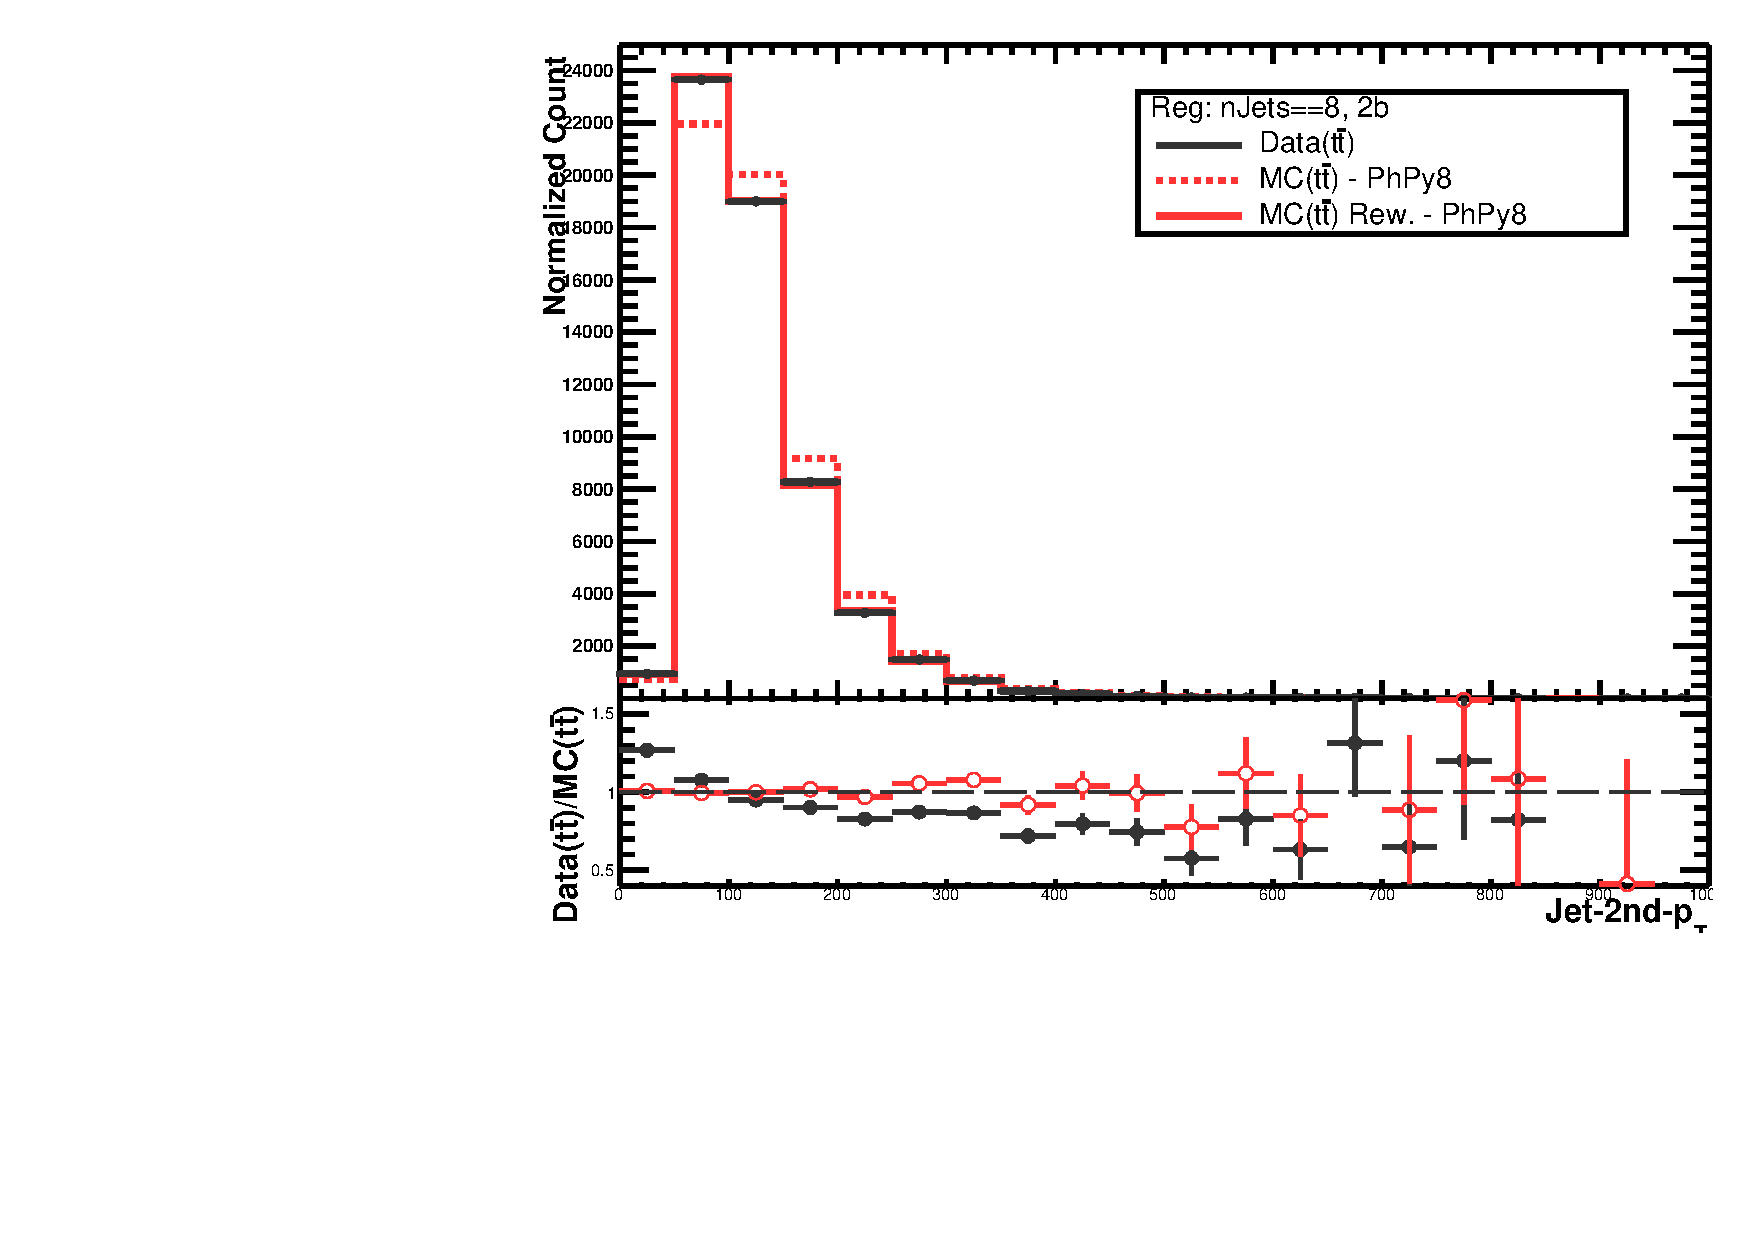
\includegraphics[width=0.24 \textwidth]{figures/rew_datamc_hfinckin_212169/1_ratiojet_pt_1__1e3_nJetsee8__1LOS.pdf} &
    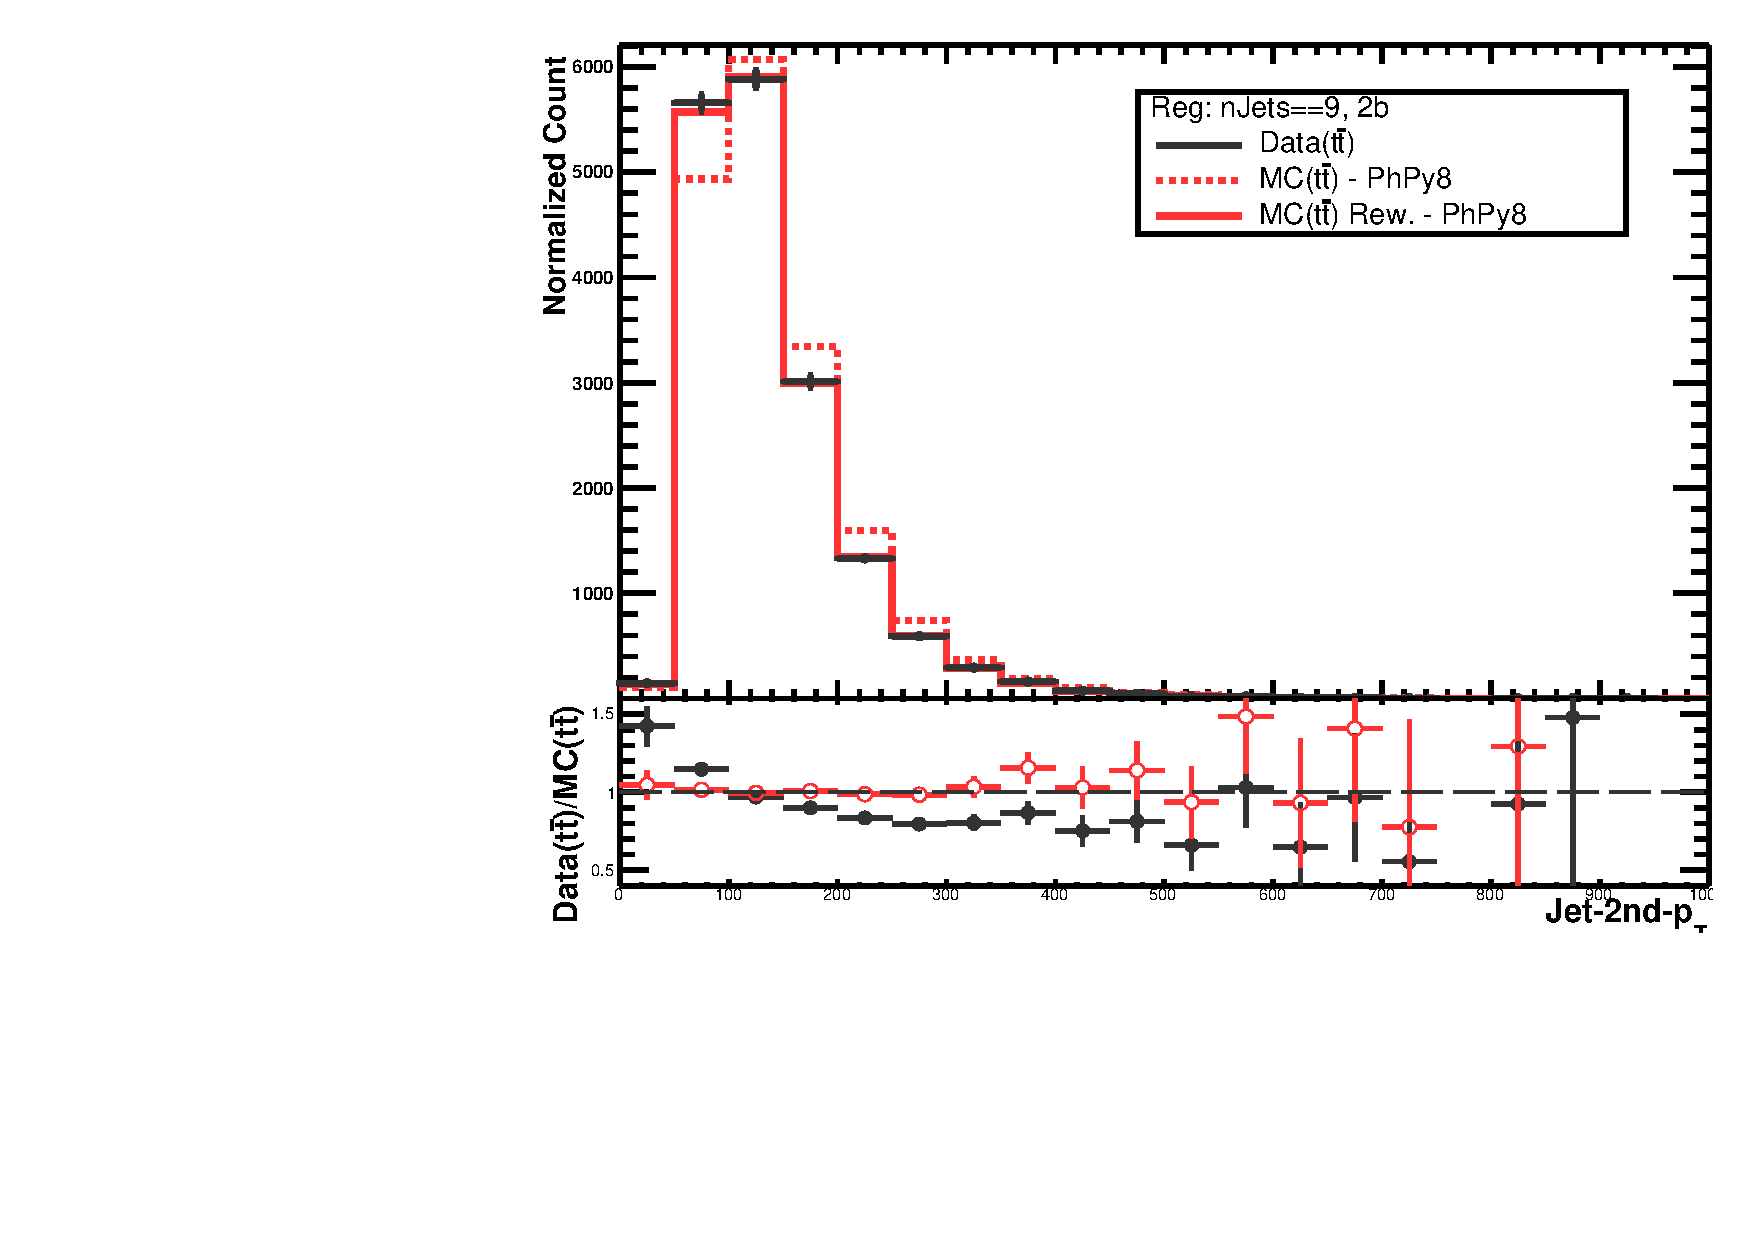
\includegraphics[width=0.24 \textwidth]{figures/rew_datamc_hfinckin_212169/1_ratiojet_pt_1__1e3_nJetsee9__1LOS.pdf} &
    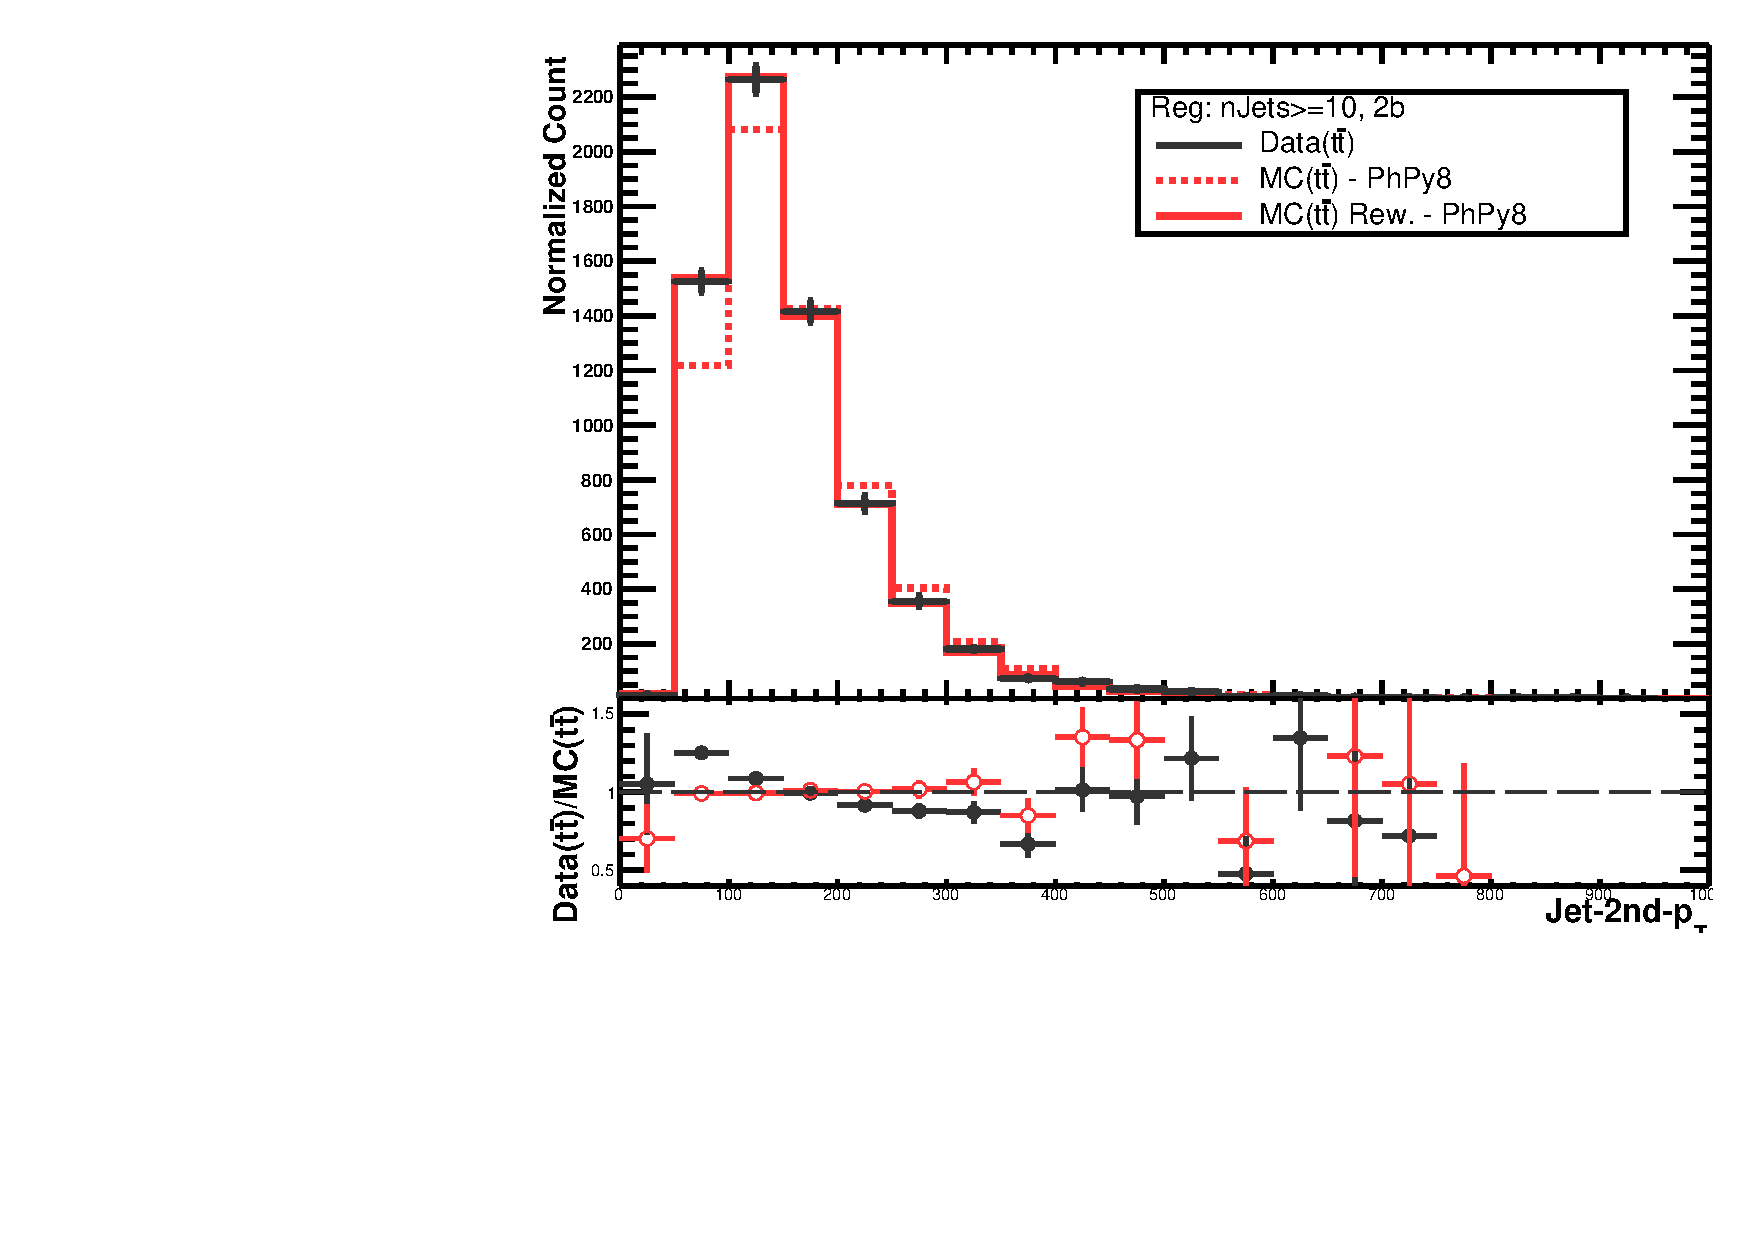
\includegraphics[width=0.24 \textwidth]{figures/rew_datamc_hfinckin_212169/1_ratiojet_pt_1__1e3_nJetsge10__1LOS.pdf} \\

    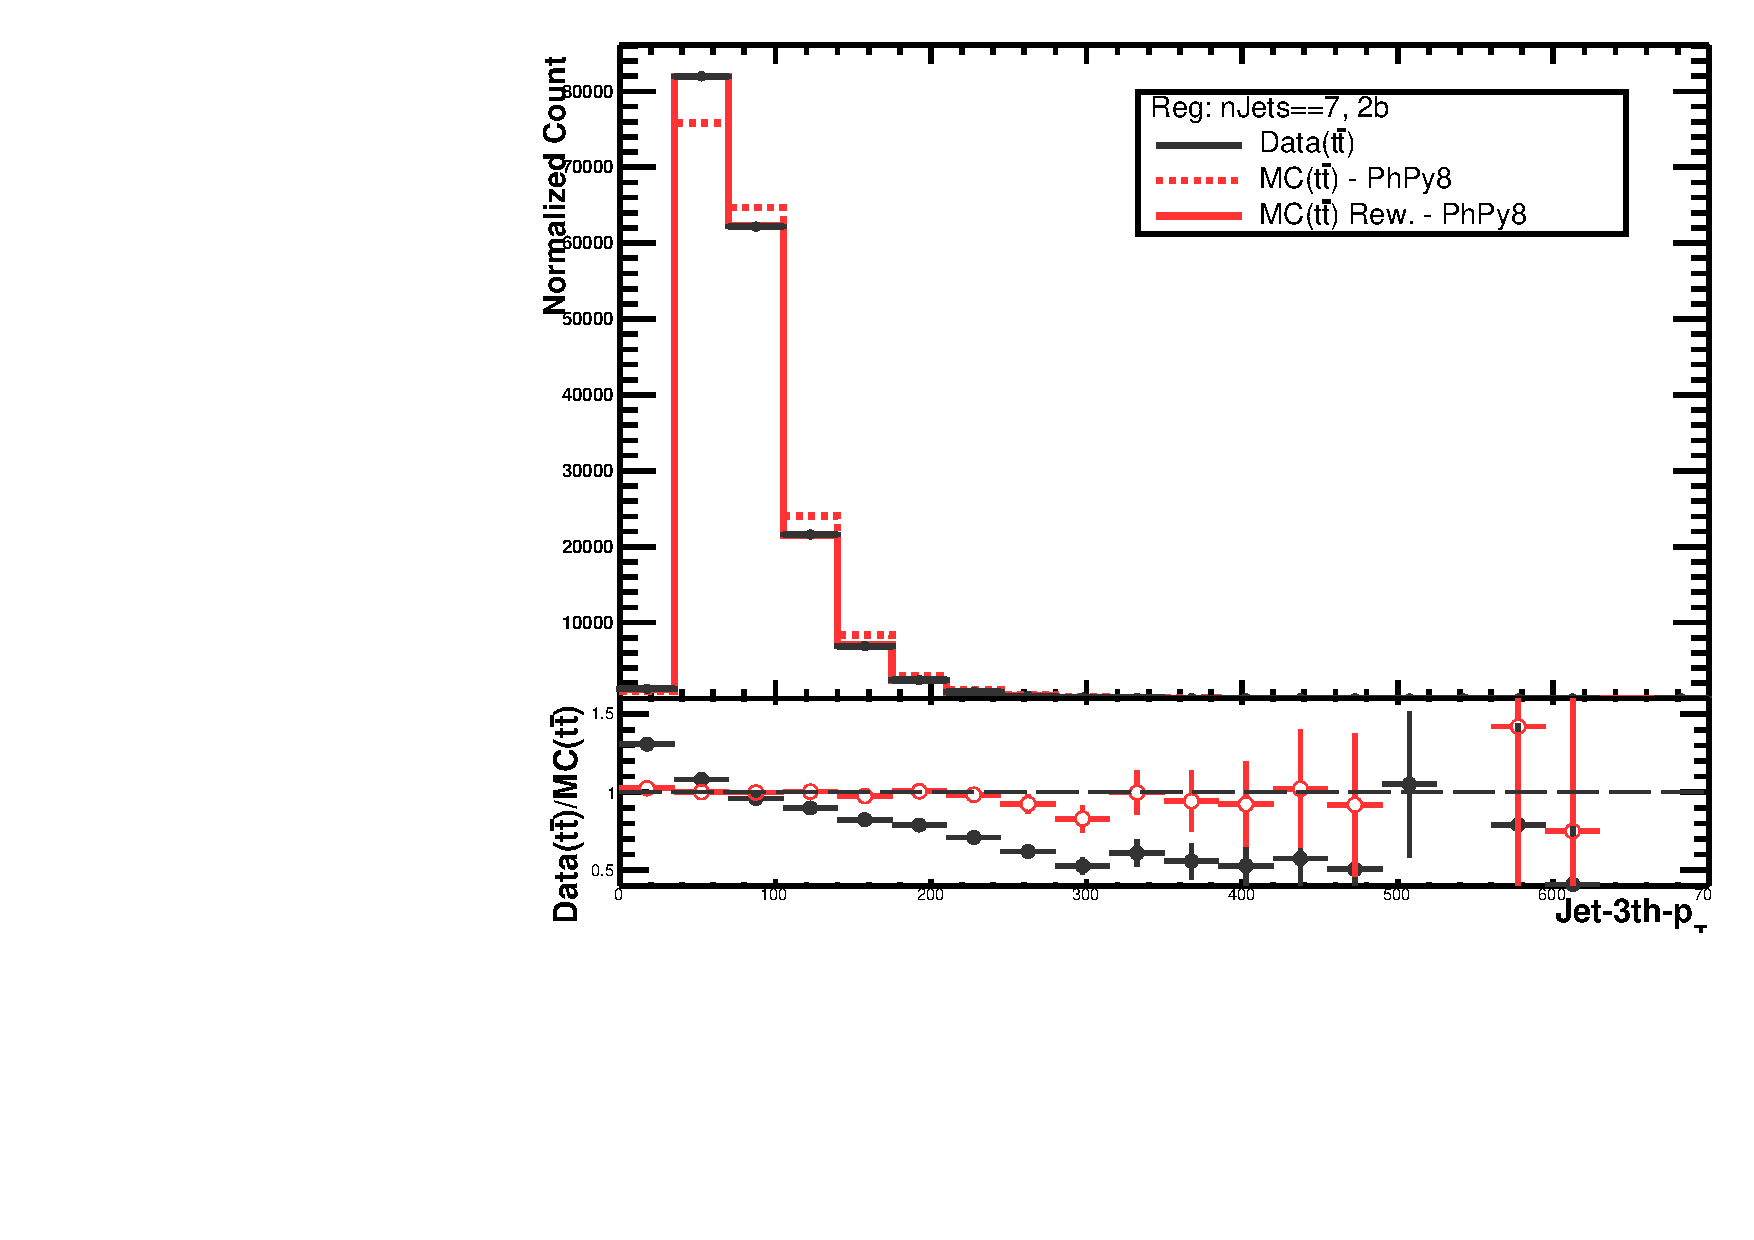
\includegraphics[width=0.24 \textwidth]{figures/rew_datamc_hfinckin_212169/1_ratiojet_pt_2__1e3_nJetsee7__1LOS.pdf} &
    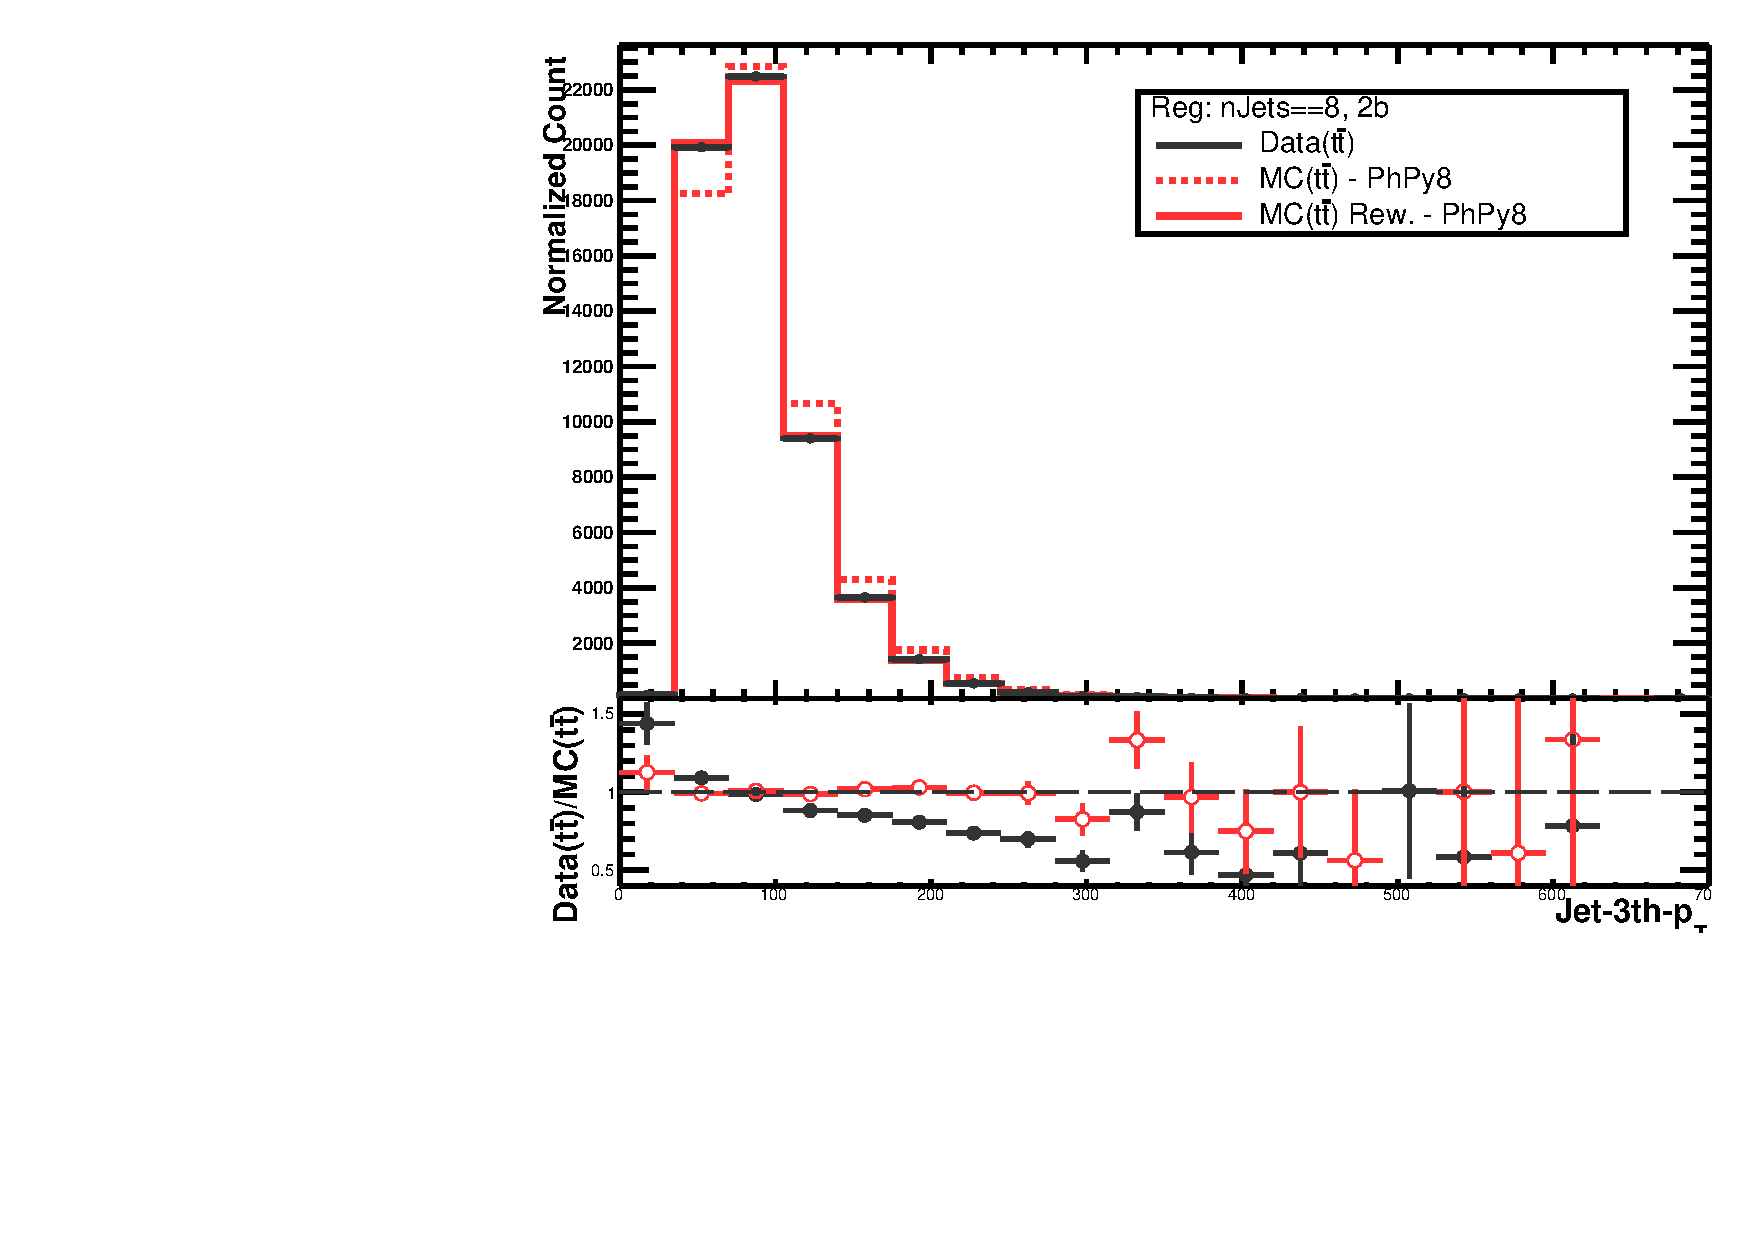
\includegraphics[width=0.24 \textwidth]{figures/rew_datamc_hfinckin_212169/1_ratiojet_pt_2__1e3_nJetsee8__1LOS.pdf} &
    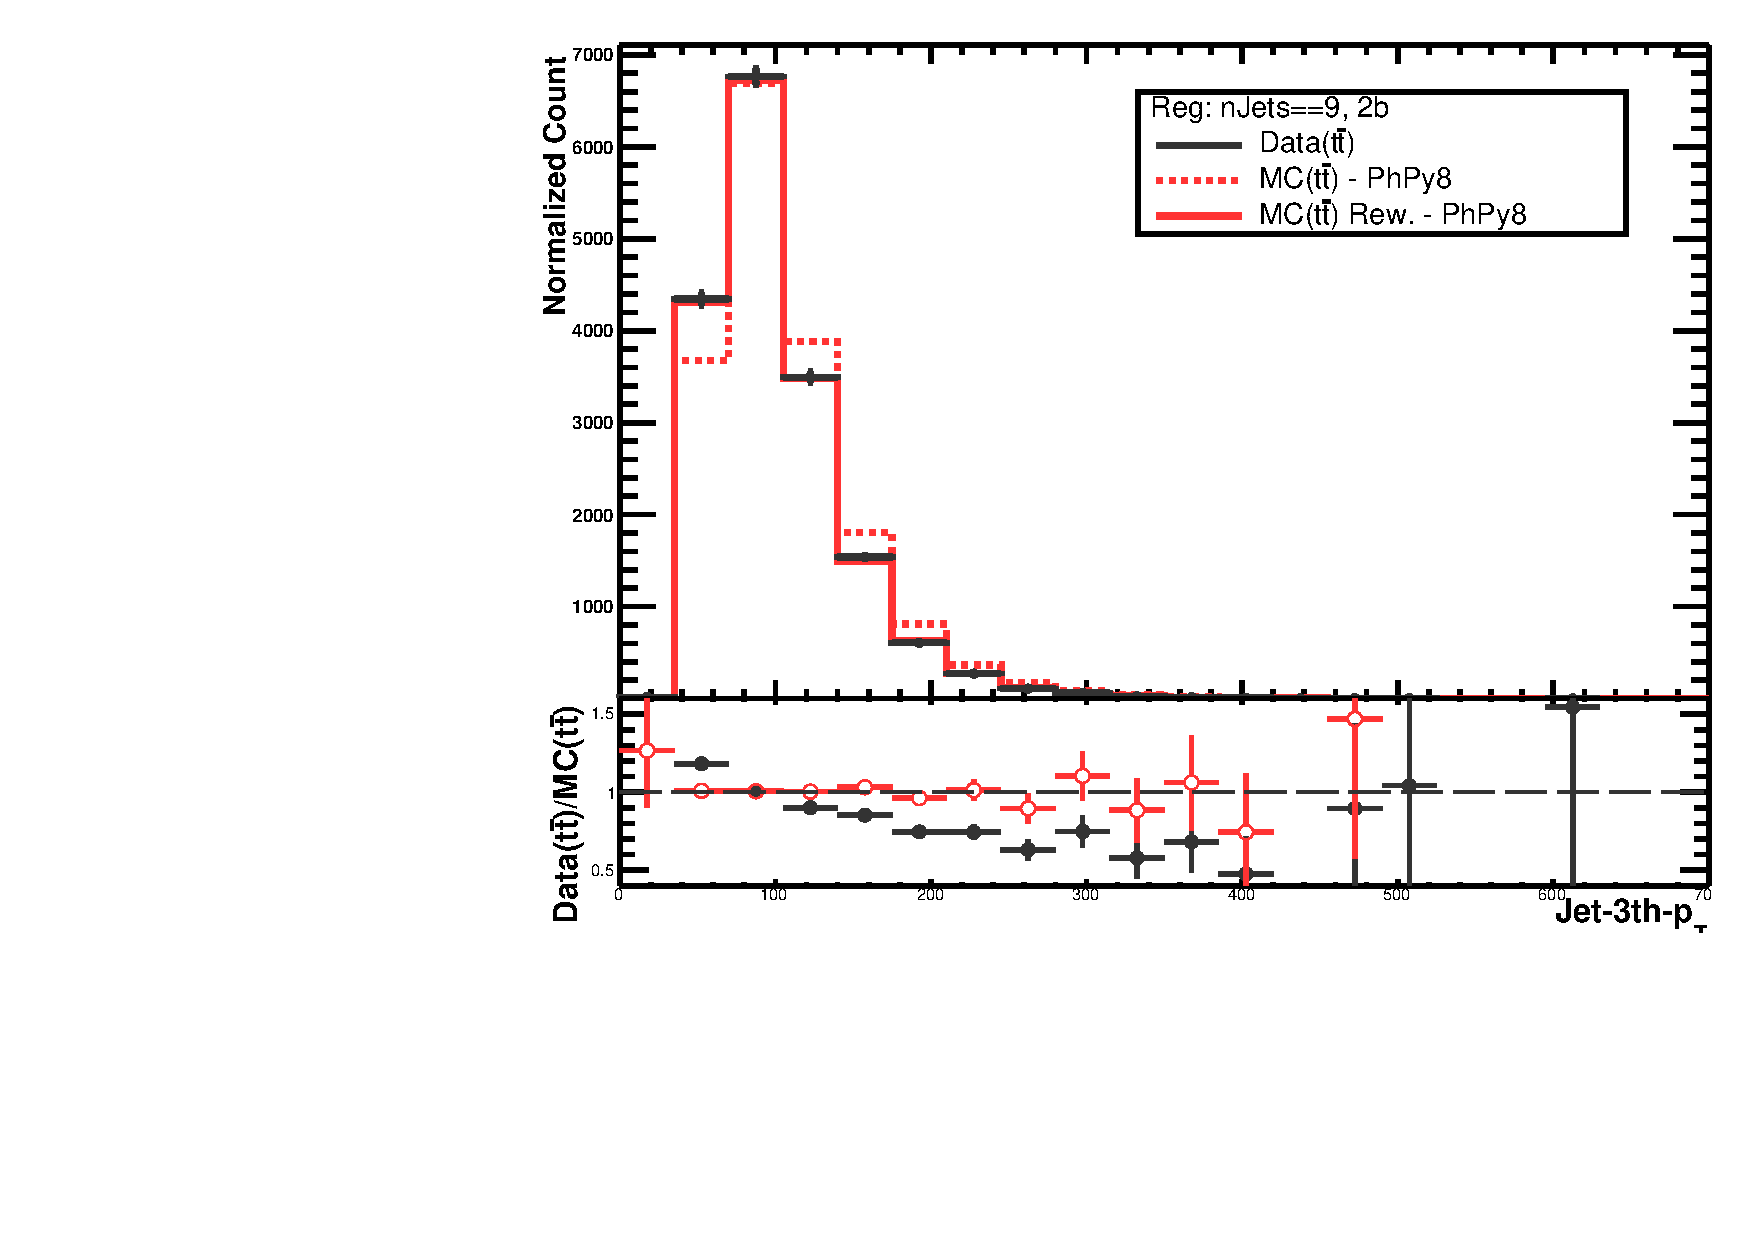
\includegraphics[width=0.24 \textwidth]{figures/rew_datamc_hfinckin_212169/1_ratiojet_pt_2__1e3_nJetsee9__1LOS.pdf} &
    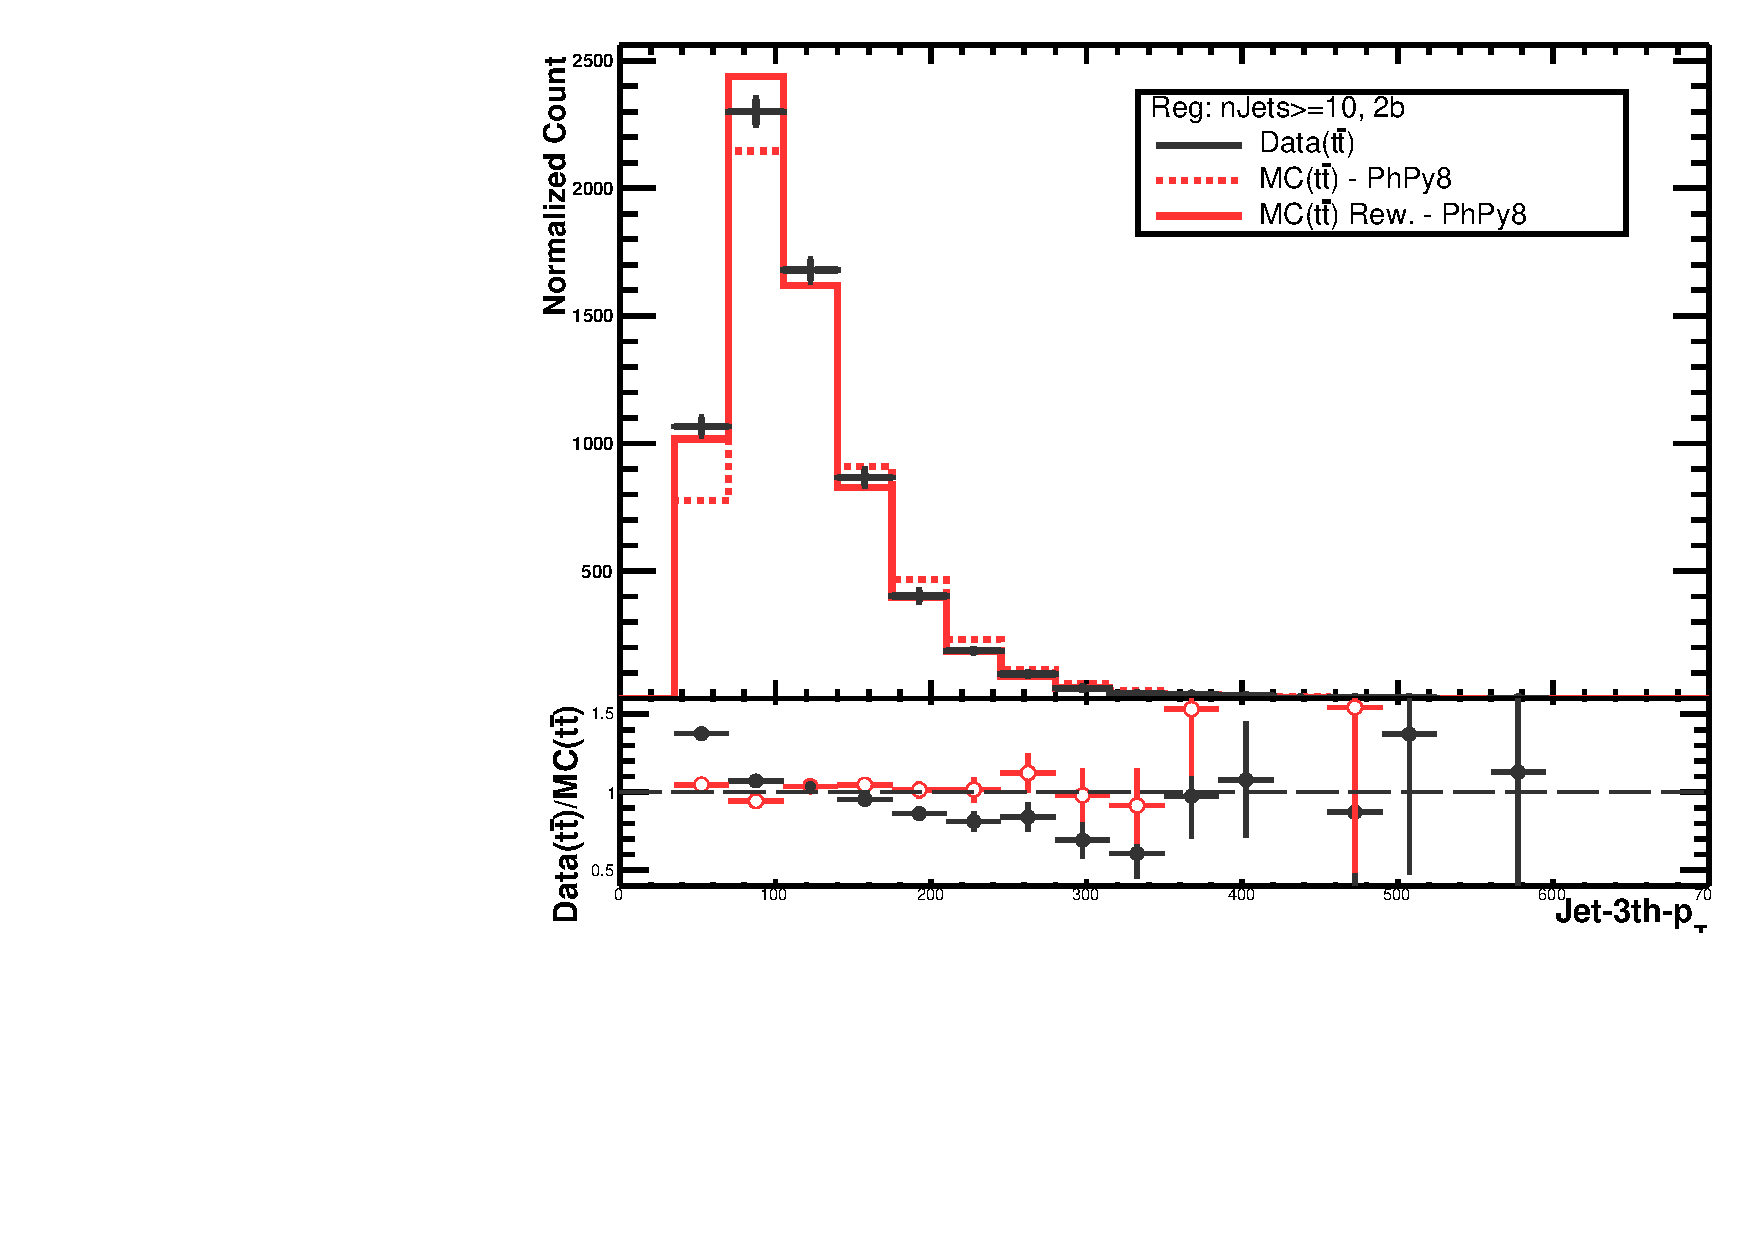
\includegraphics[width=0.24 \textwidth]{figures/rew_datamc_hfinckin_212169/1_ratiojet_pt_2__1e3_nJetsge10__1LOS.pdf} \\

    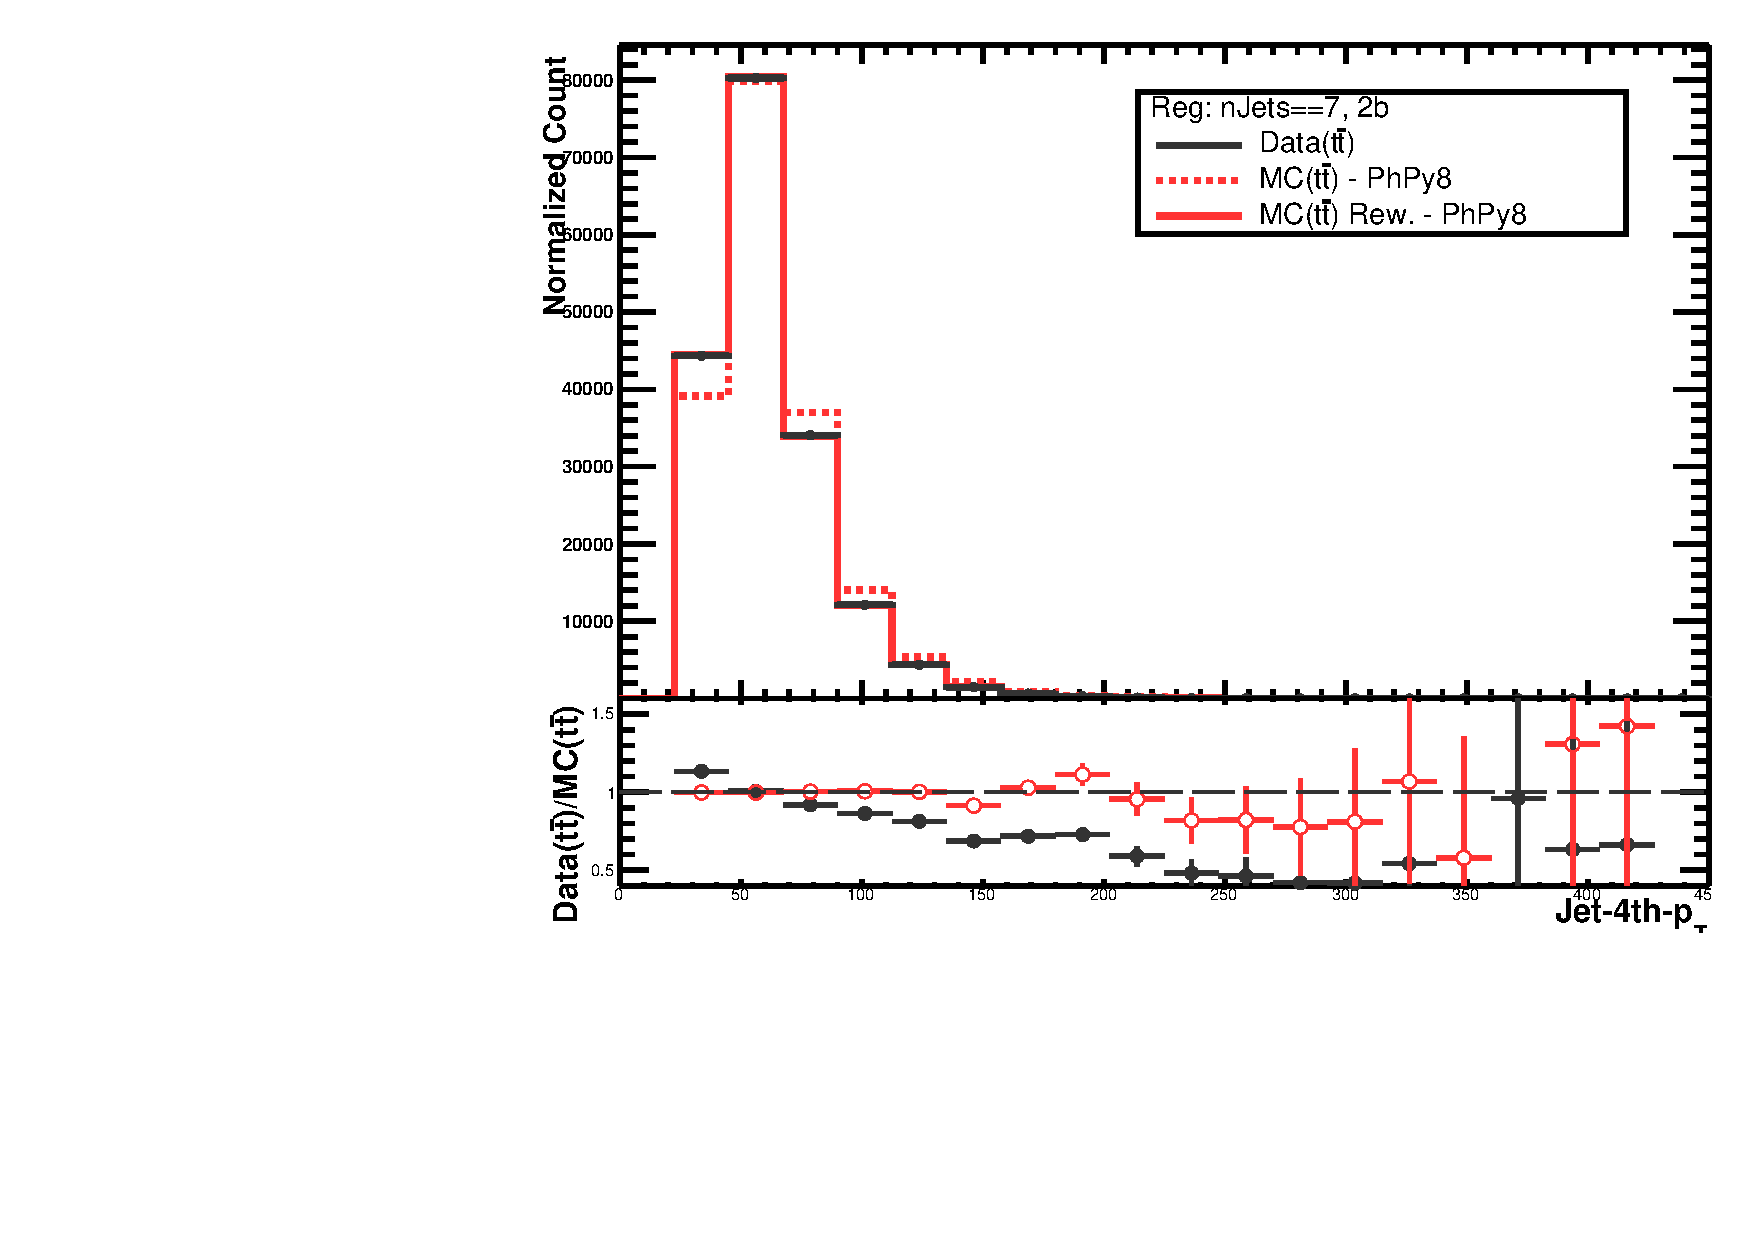
\includegraphics[width=0.24 \textwidth]{figures/rew_datamc_hfinckin_212169/1_ratiojet_pt_3__1e3_nJetsee7__1LOS.pdf} &
    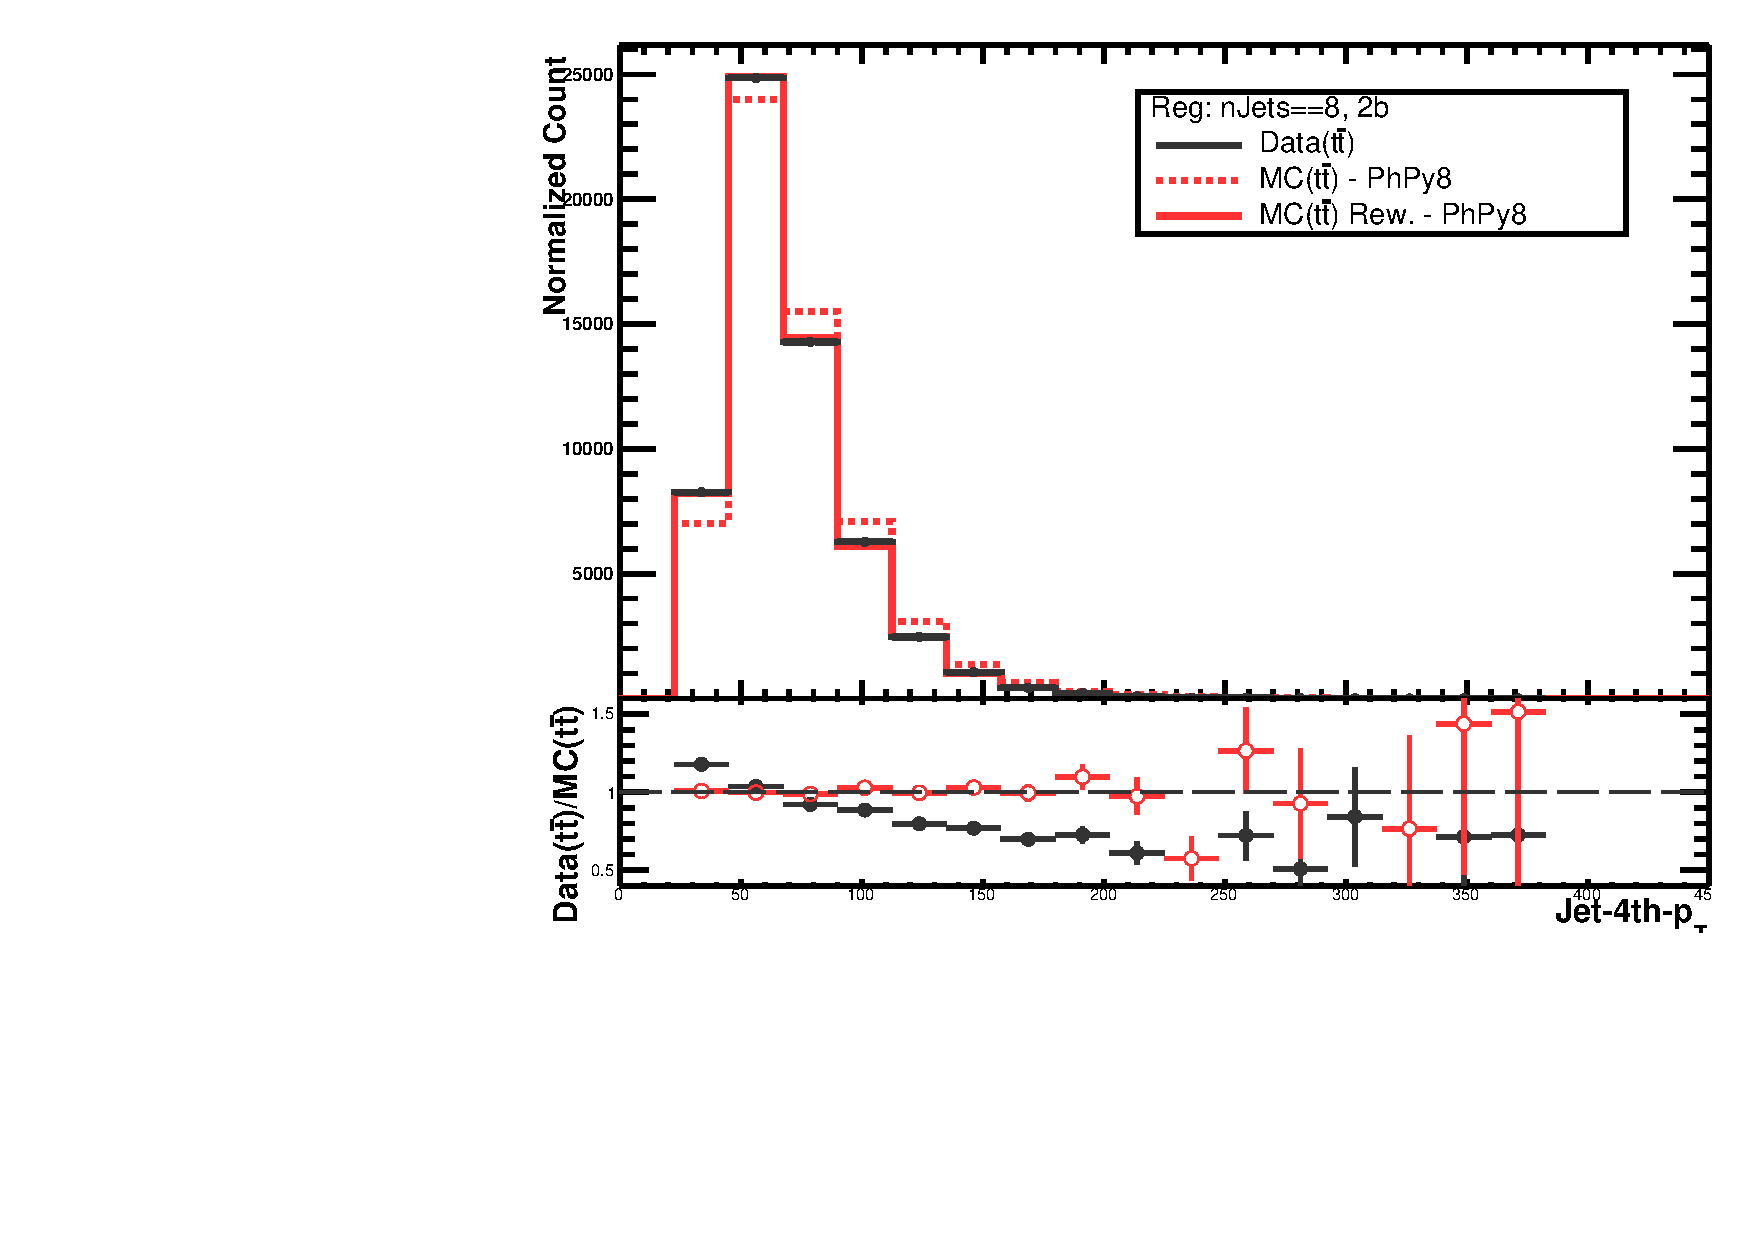
\includegraphics[width=0.24 \textwidth]{figures/rew_datamc_hfinckin_212169/1_ratiojet_pt_3__1e3_nJetsee8__1LOS.pdf} &
    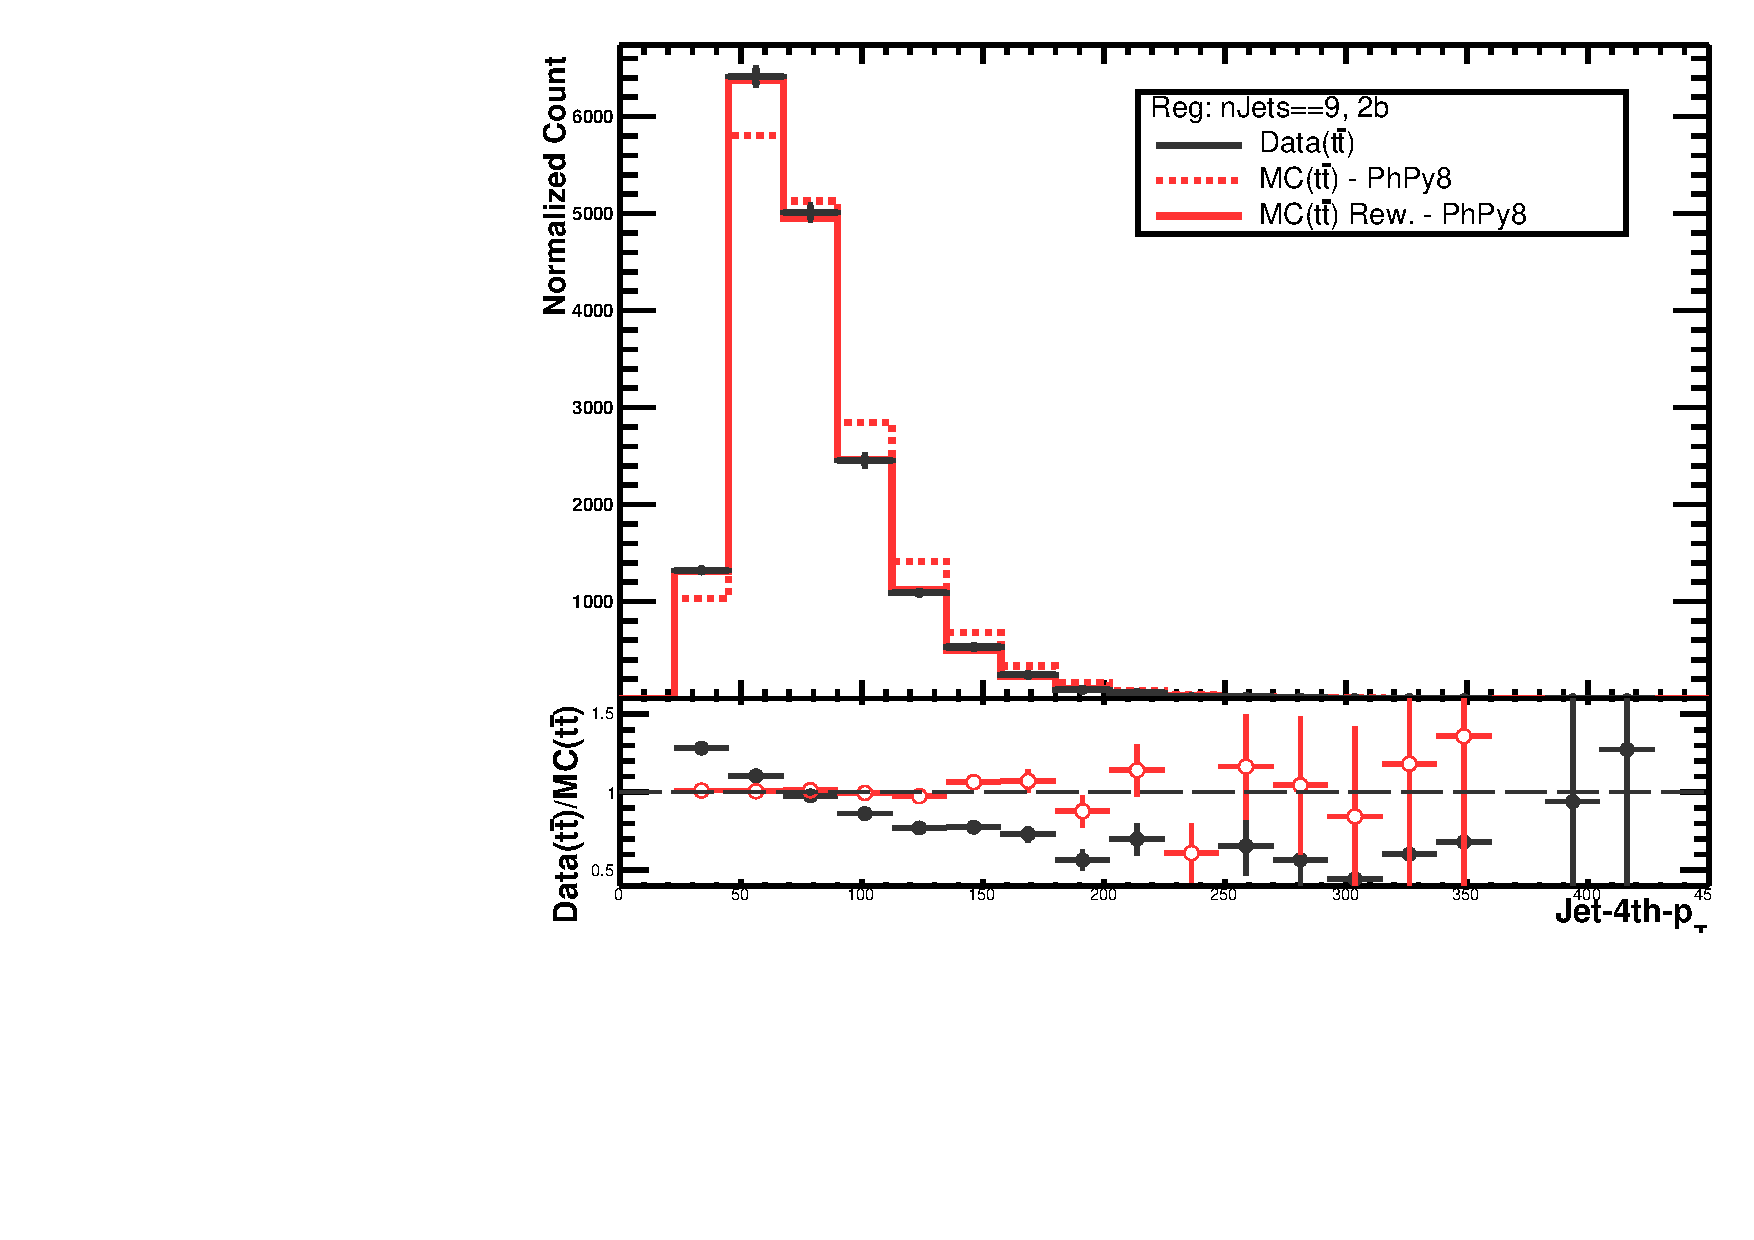
\includegraphics[width=0.24 \textwidth]{figures/rew_datamc_hfinckin_212169/1_ratiojet_pt_3__1e3_nJetsee9__1LOS.pdf} &
    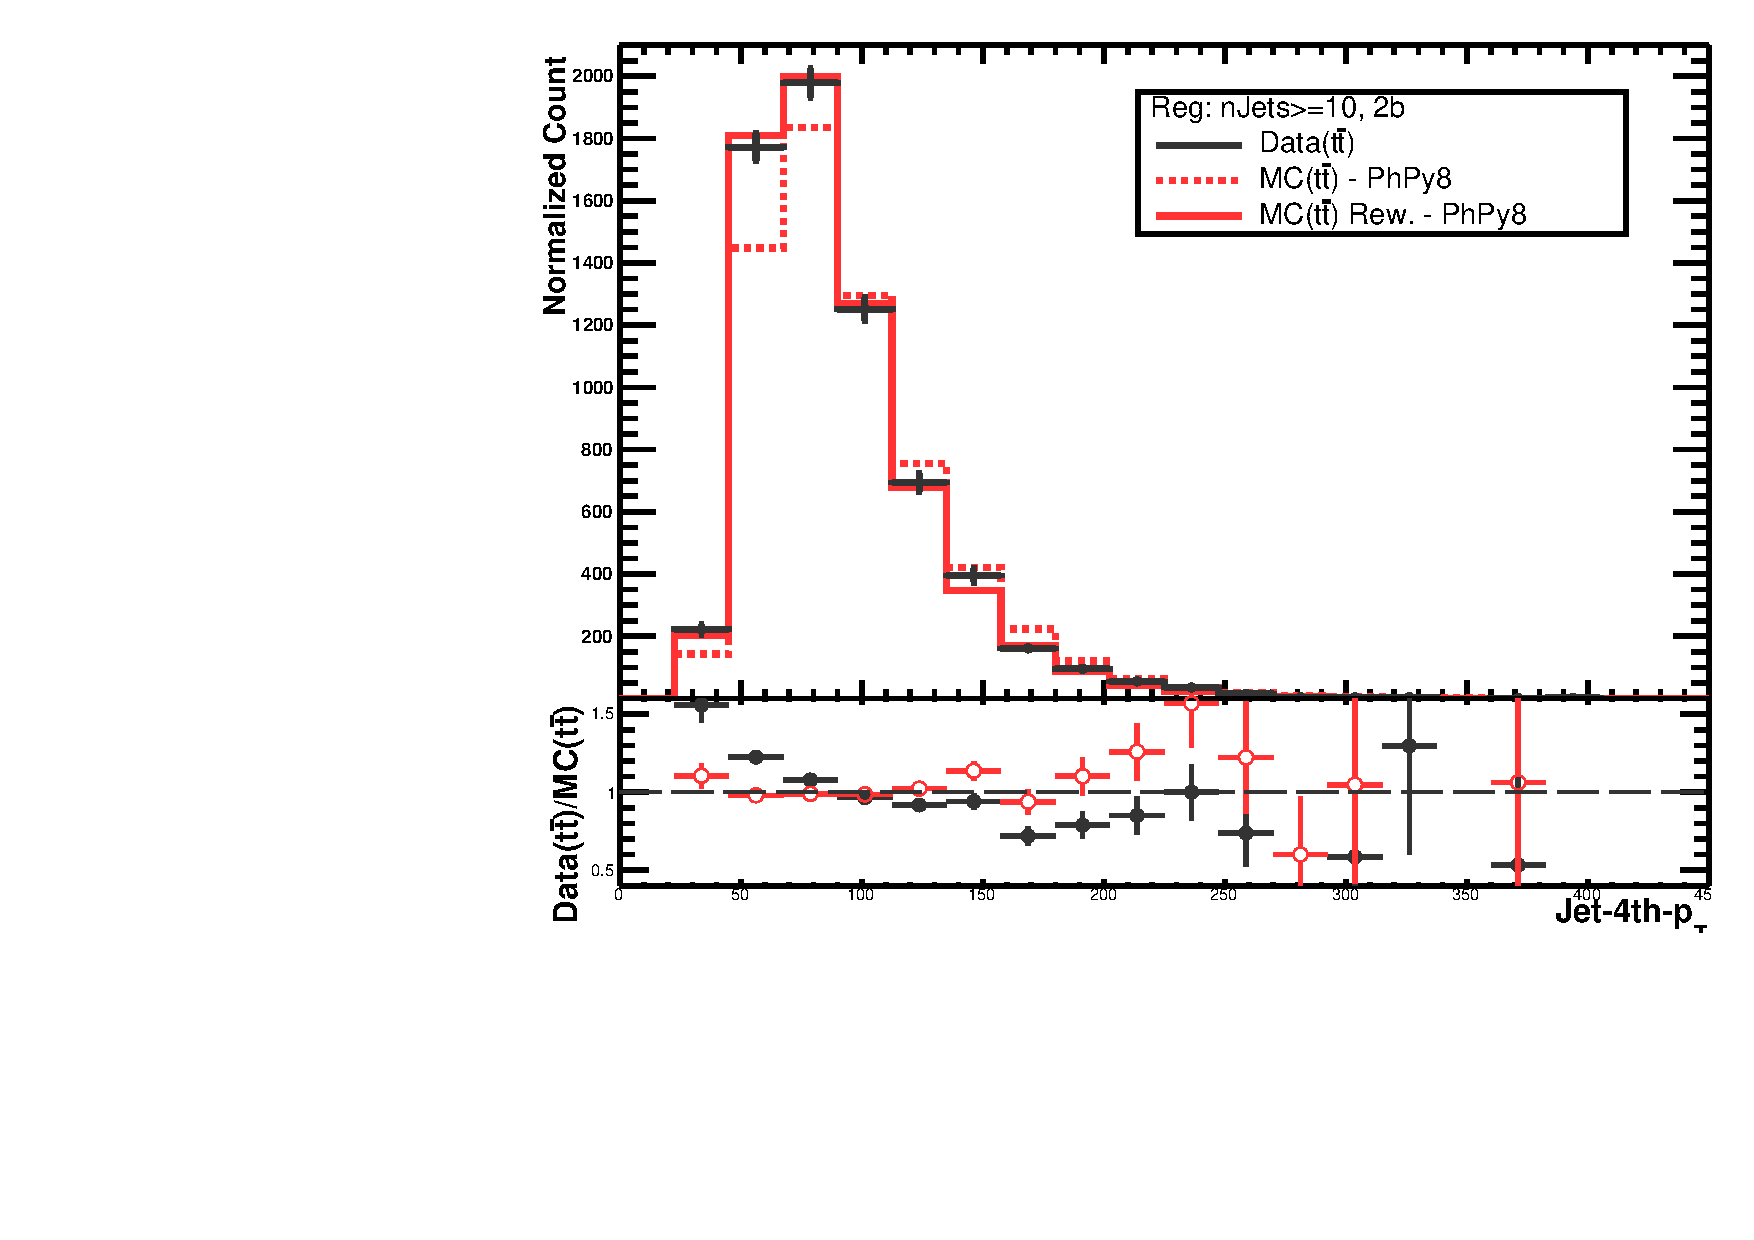
\includegraphics[width=0.24 \textwidth]{figures/rew_datamc_hfinckin_212169/1_ratiojet_pt_3__1e3_nJetsge10__1LOS.pdf} \\

    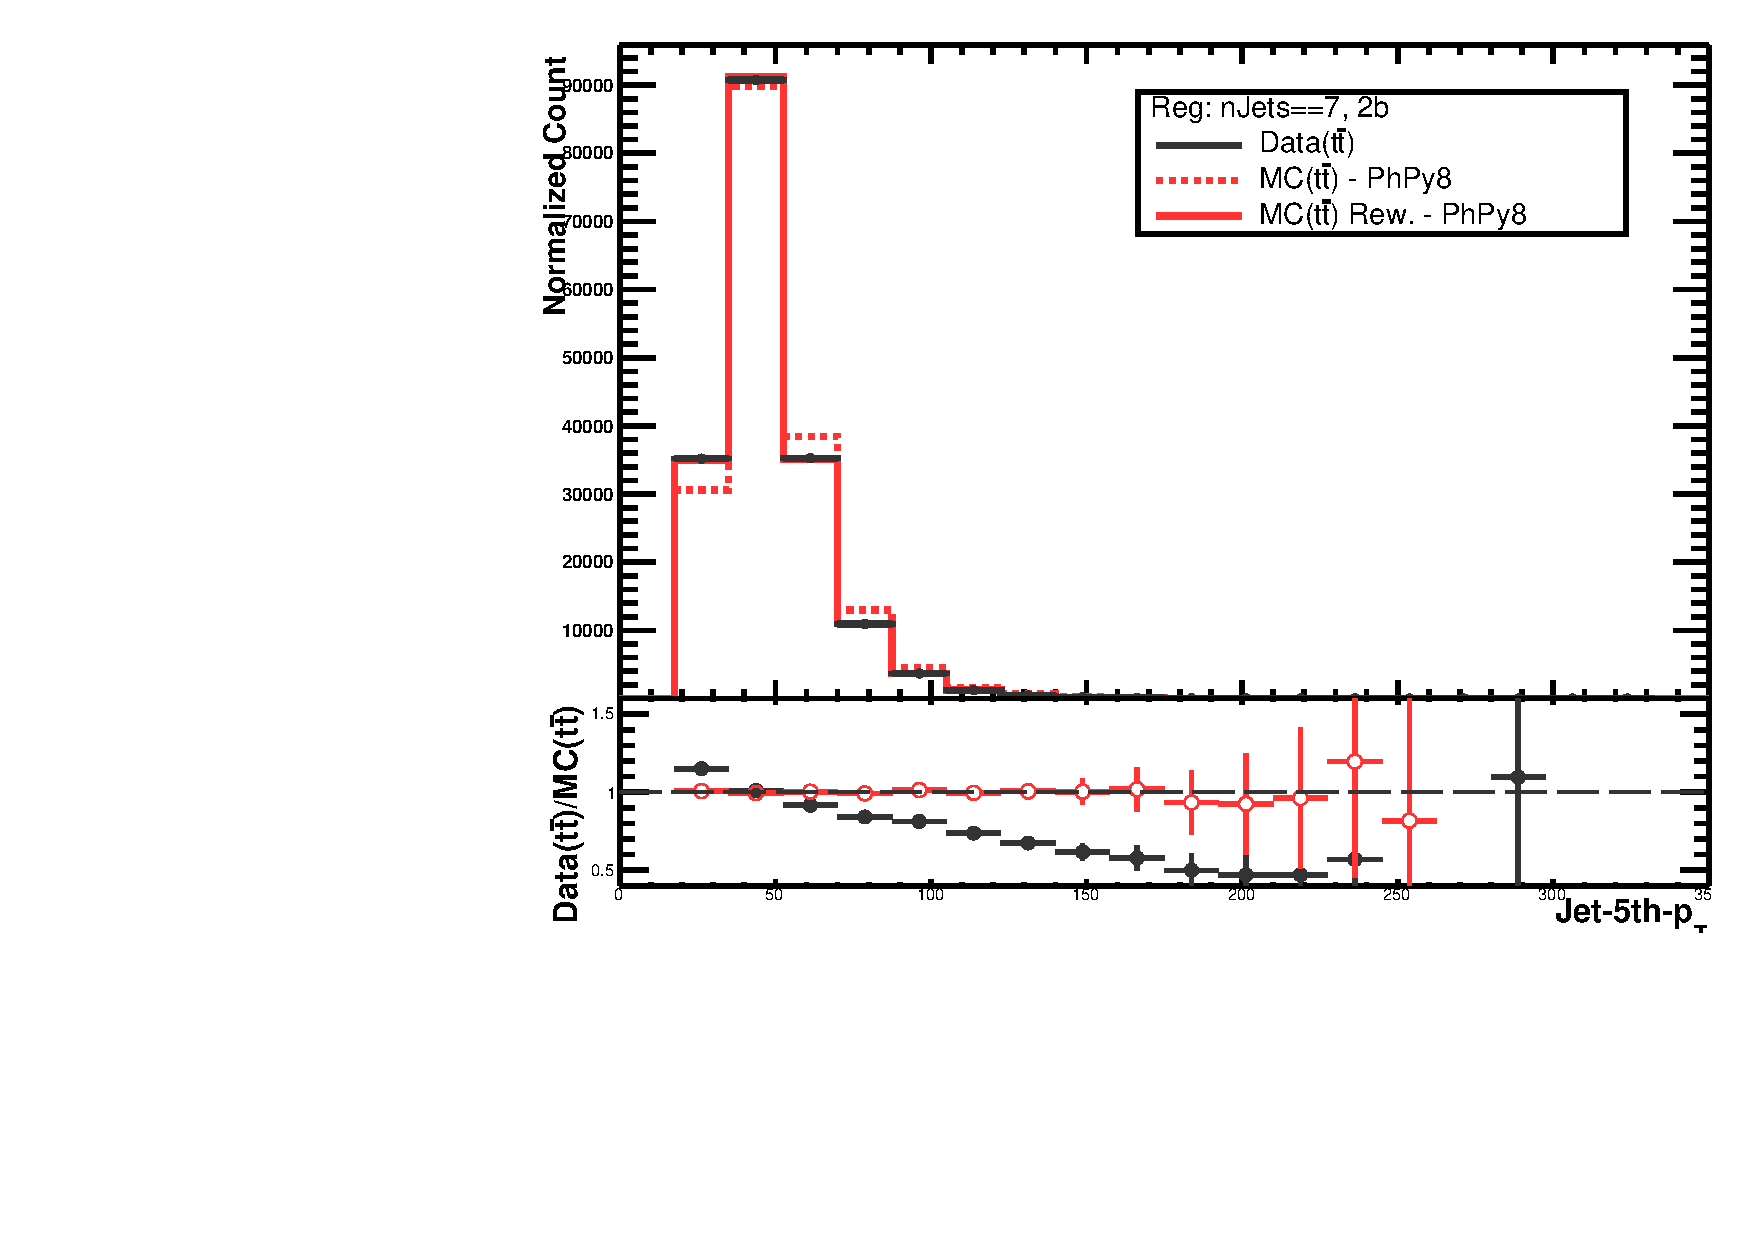
\includegraphics[width=0.24 \textwidth]{figures/rew_datamc_hfinckin_212169/1_ratiojet_pt_4__1e3_nJetsee7__1LOS.pdf} &
    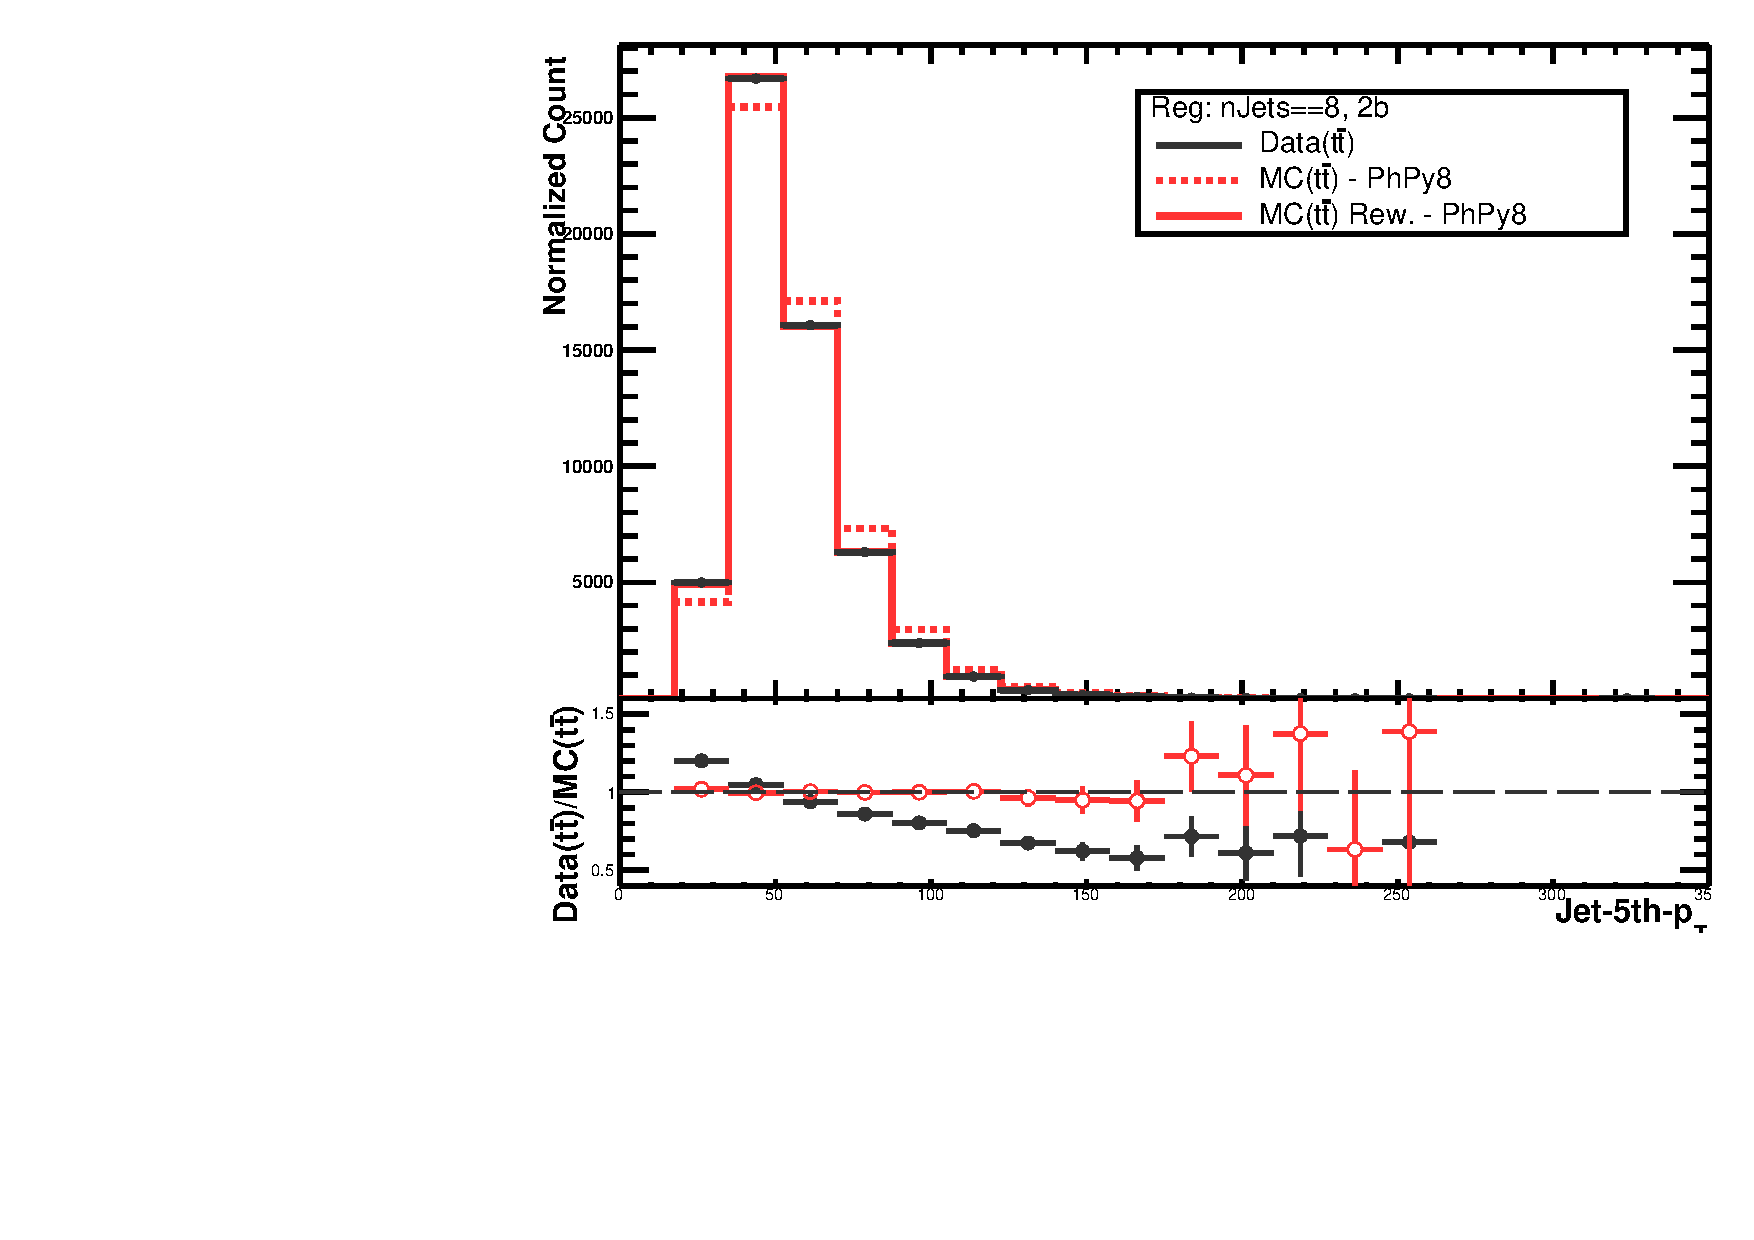
\includegraphics[width=0.24 \textwidth]{figures/rew_datamc_hfinckin_212169/1_ratiojet_pt_4__1e3_nJetsee8__1LOS.pdf} &
    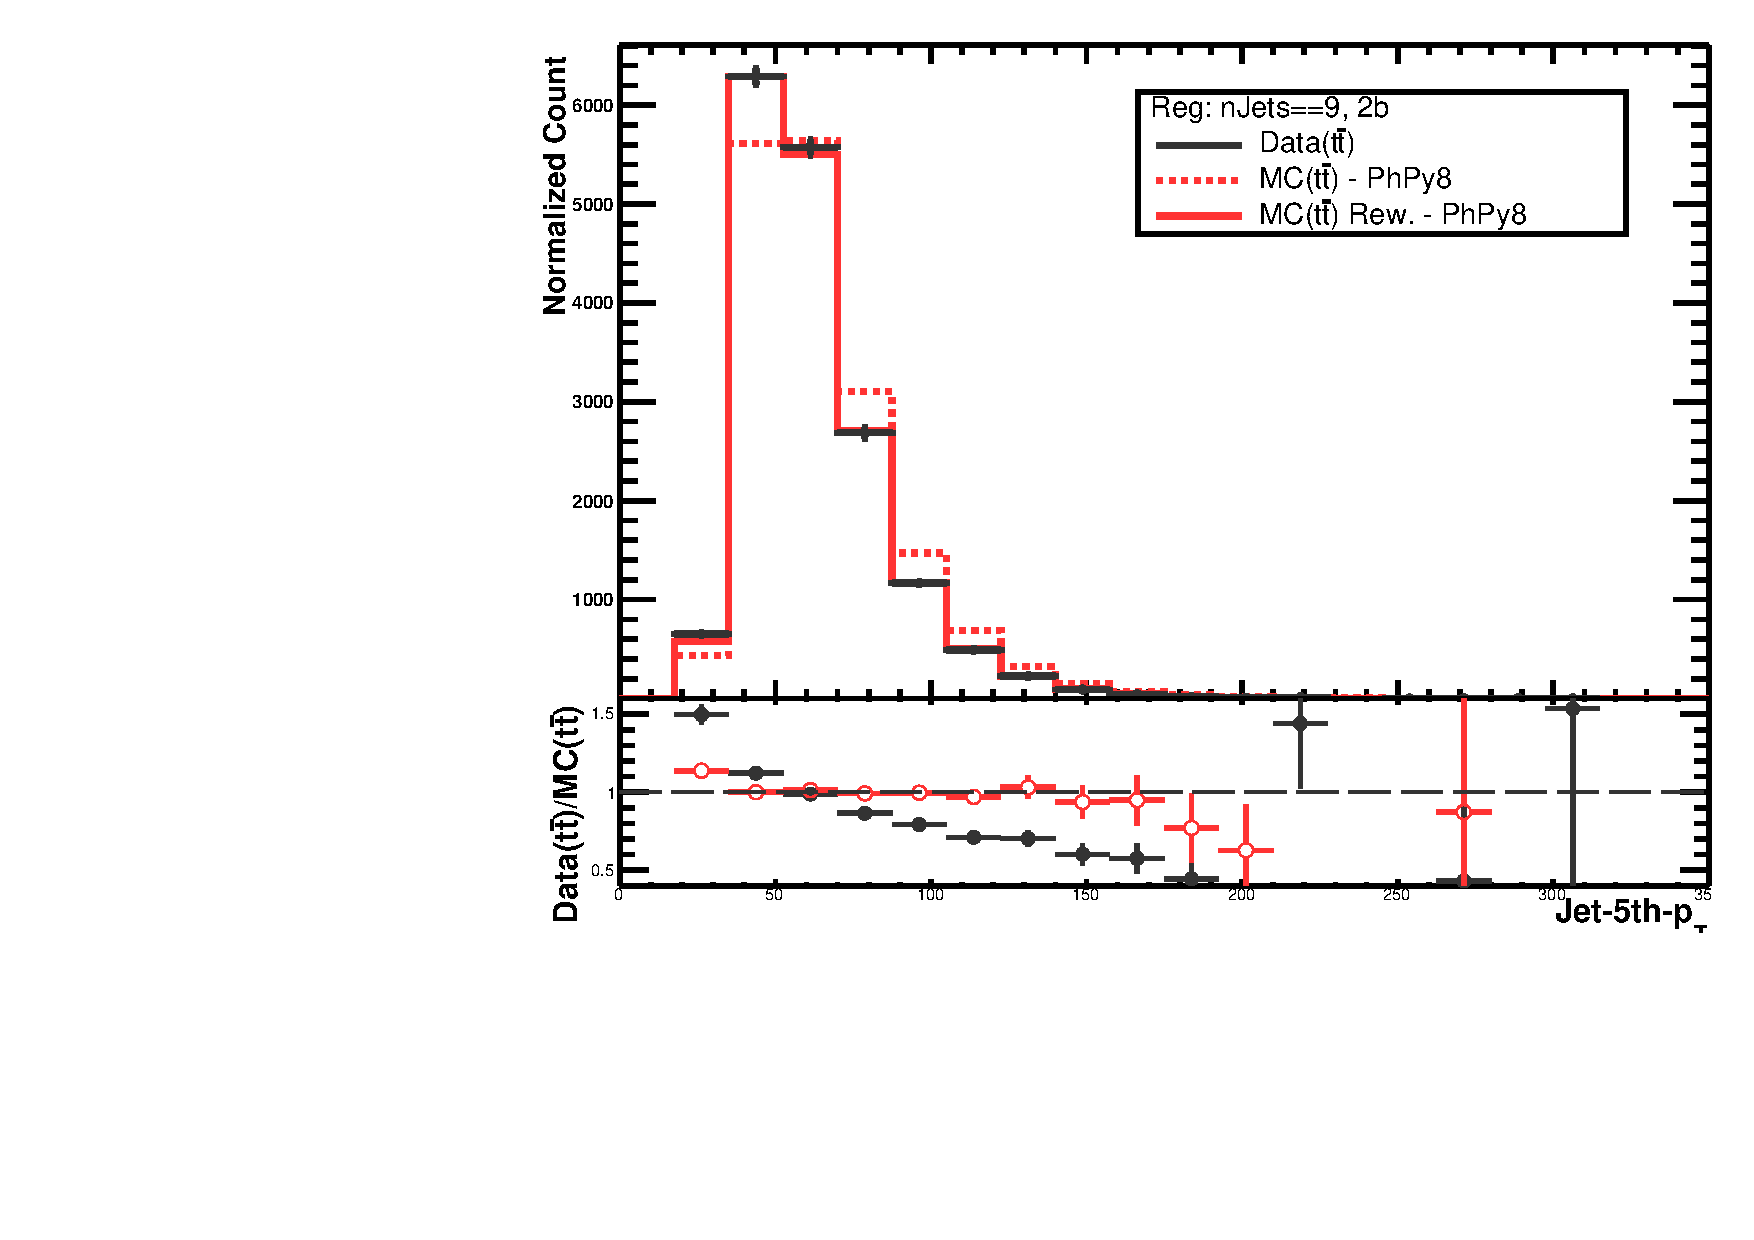
\includegraphics[width=0.24 \textwidth]{figures/rew_datamc_hfinckin_212169/1_ratiojet_pt_4__1e3_nJetsee9__1LOS.pdf} &
    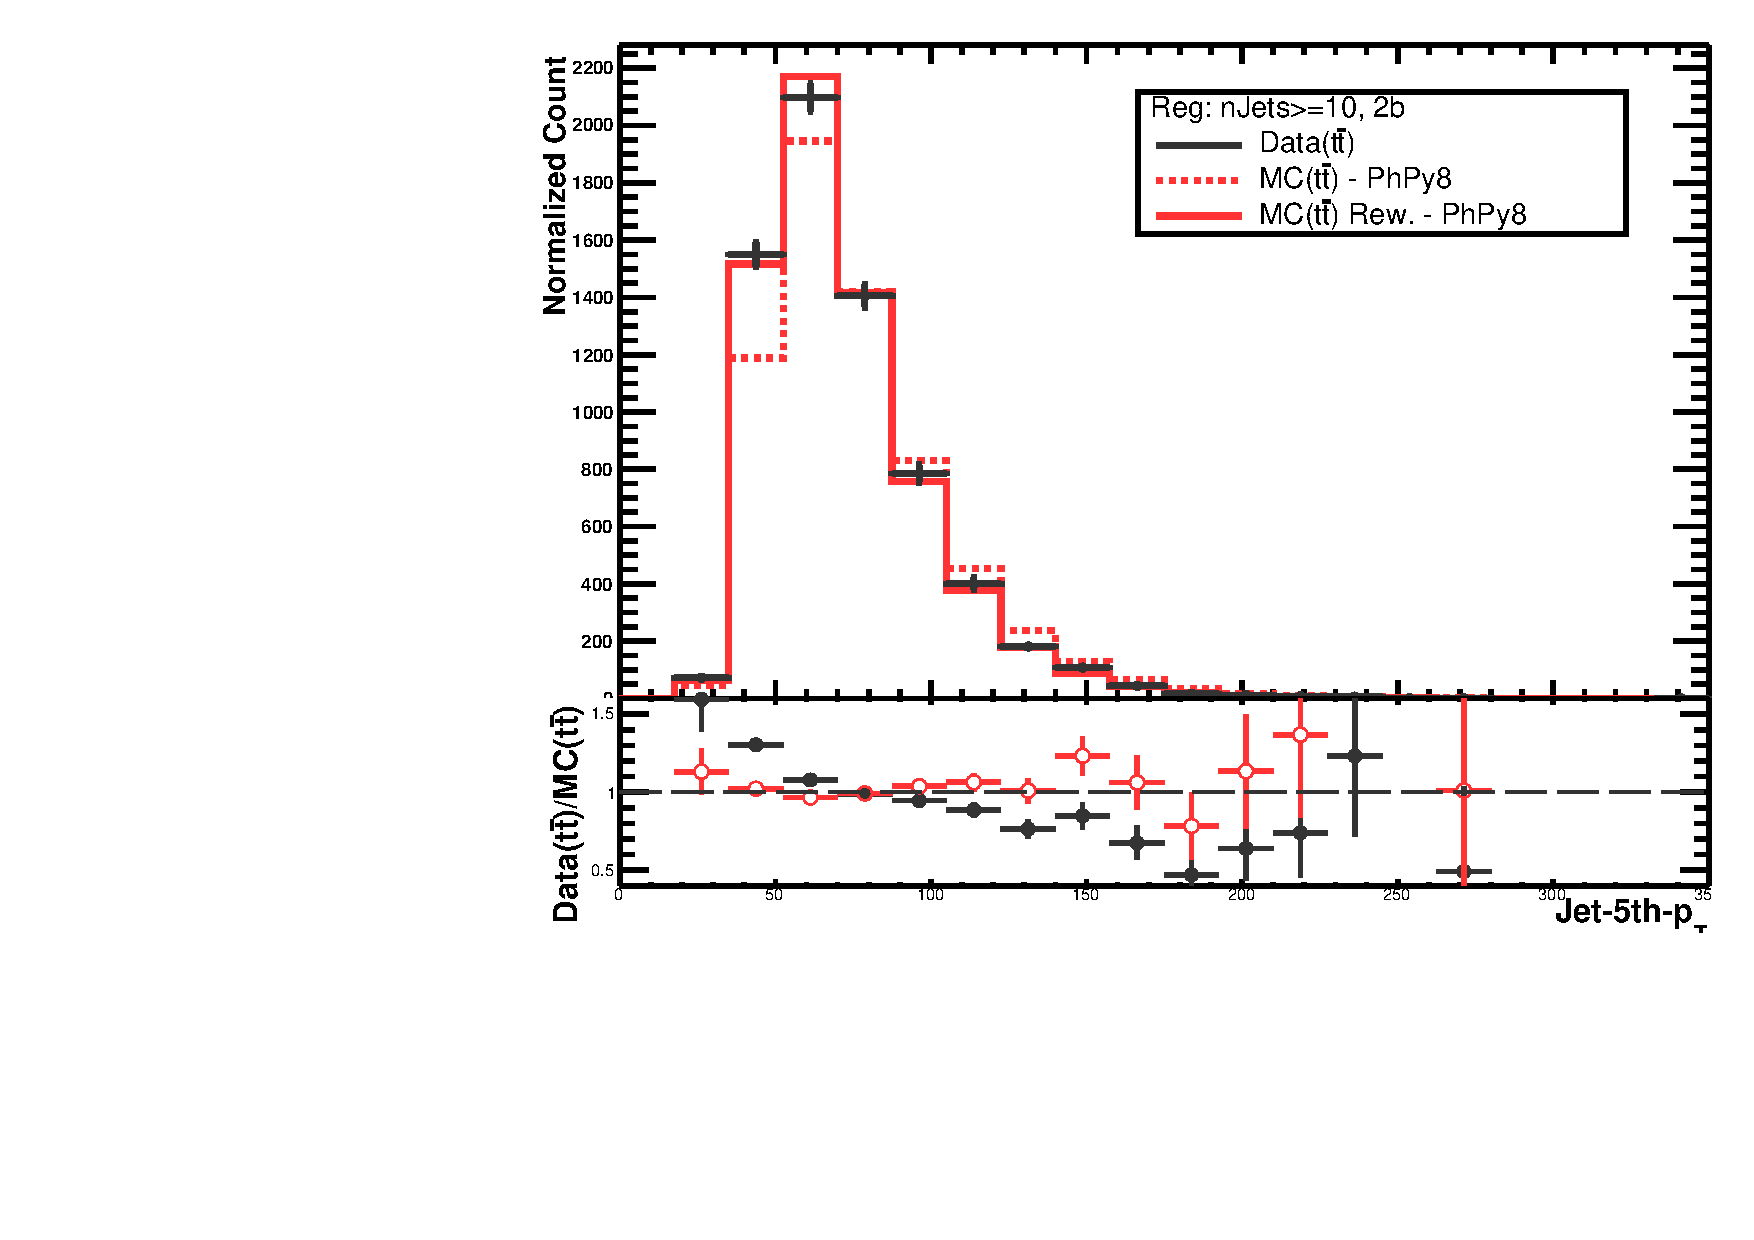
\includegraphics[width=0.24 \textwidth]{figures/rew_datamc_hfinckin_212169/1_ratiojet_pt_4__1e3_nJetsge10__1LOS.pdf} \\

    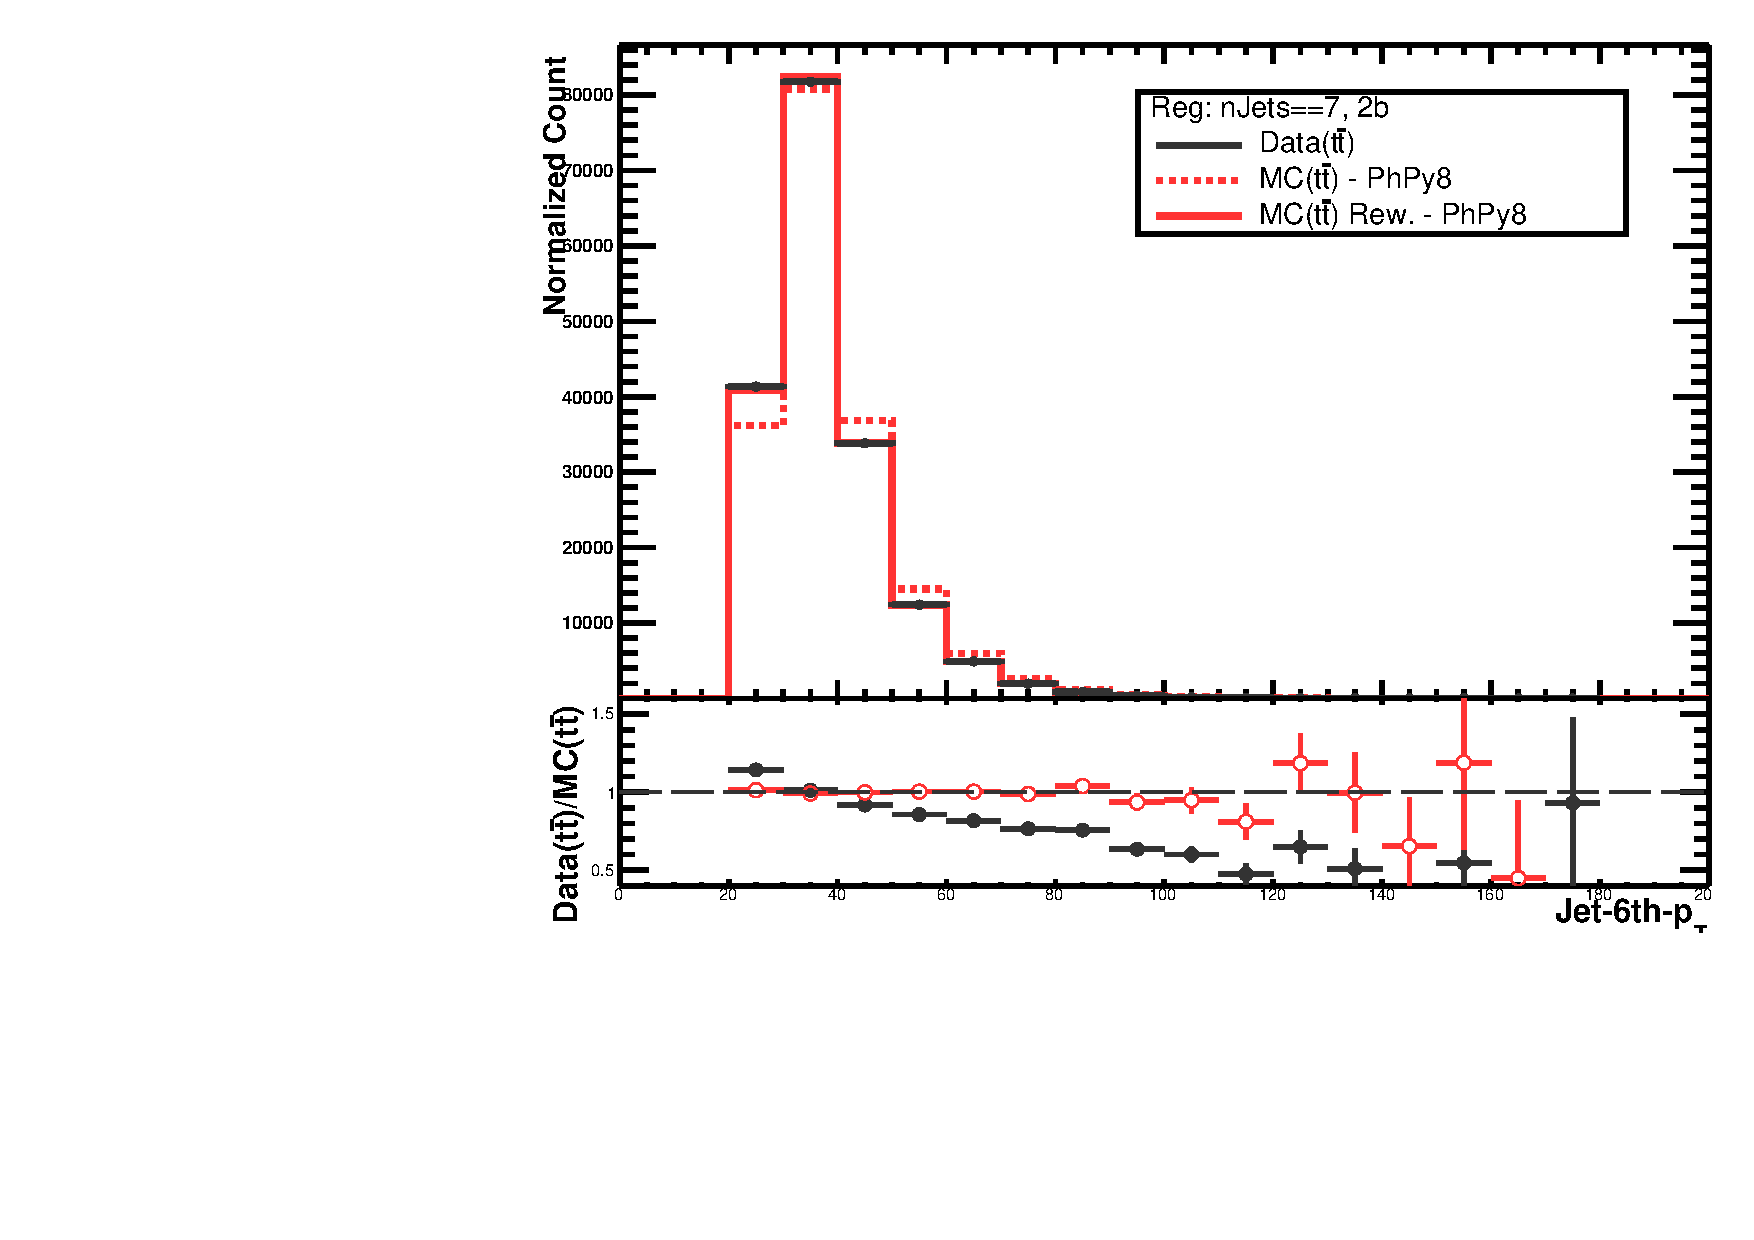
\includegraphics[width=0.24 \textwidth]{figures/rew_datamc_hfinckin_212169/1_ratiojet_pt_5__1e3_nJetsee7__1LOS.pdf} &
    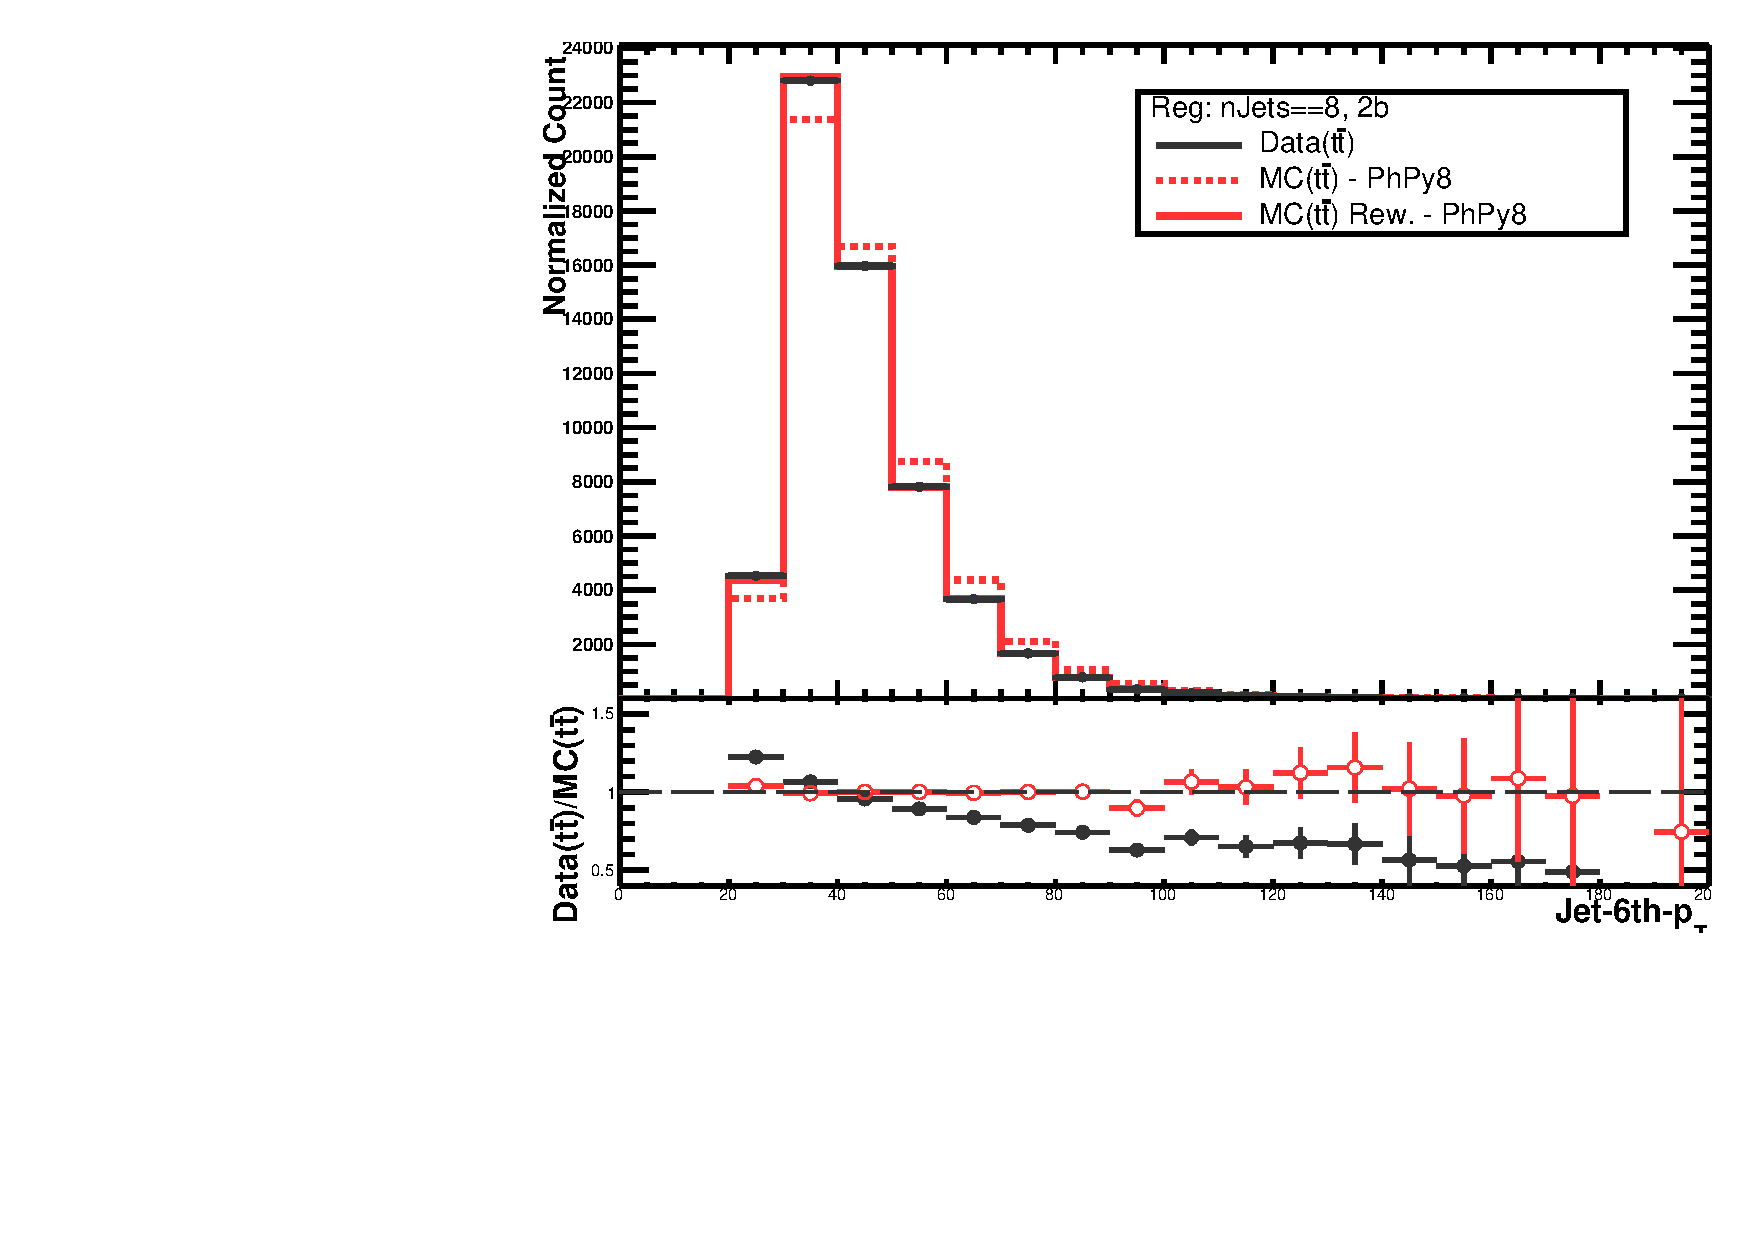
\includegraphics[width=0.24 \textwidth]{figures/rew_datamc_hfinckin_212169/1_ratiojet_pt_5__1e3_nJetsee8__1LOS.pdf} &
    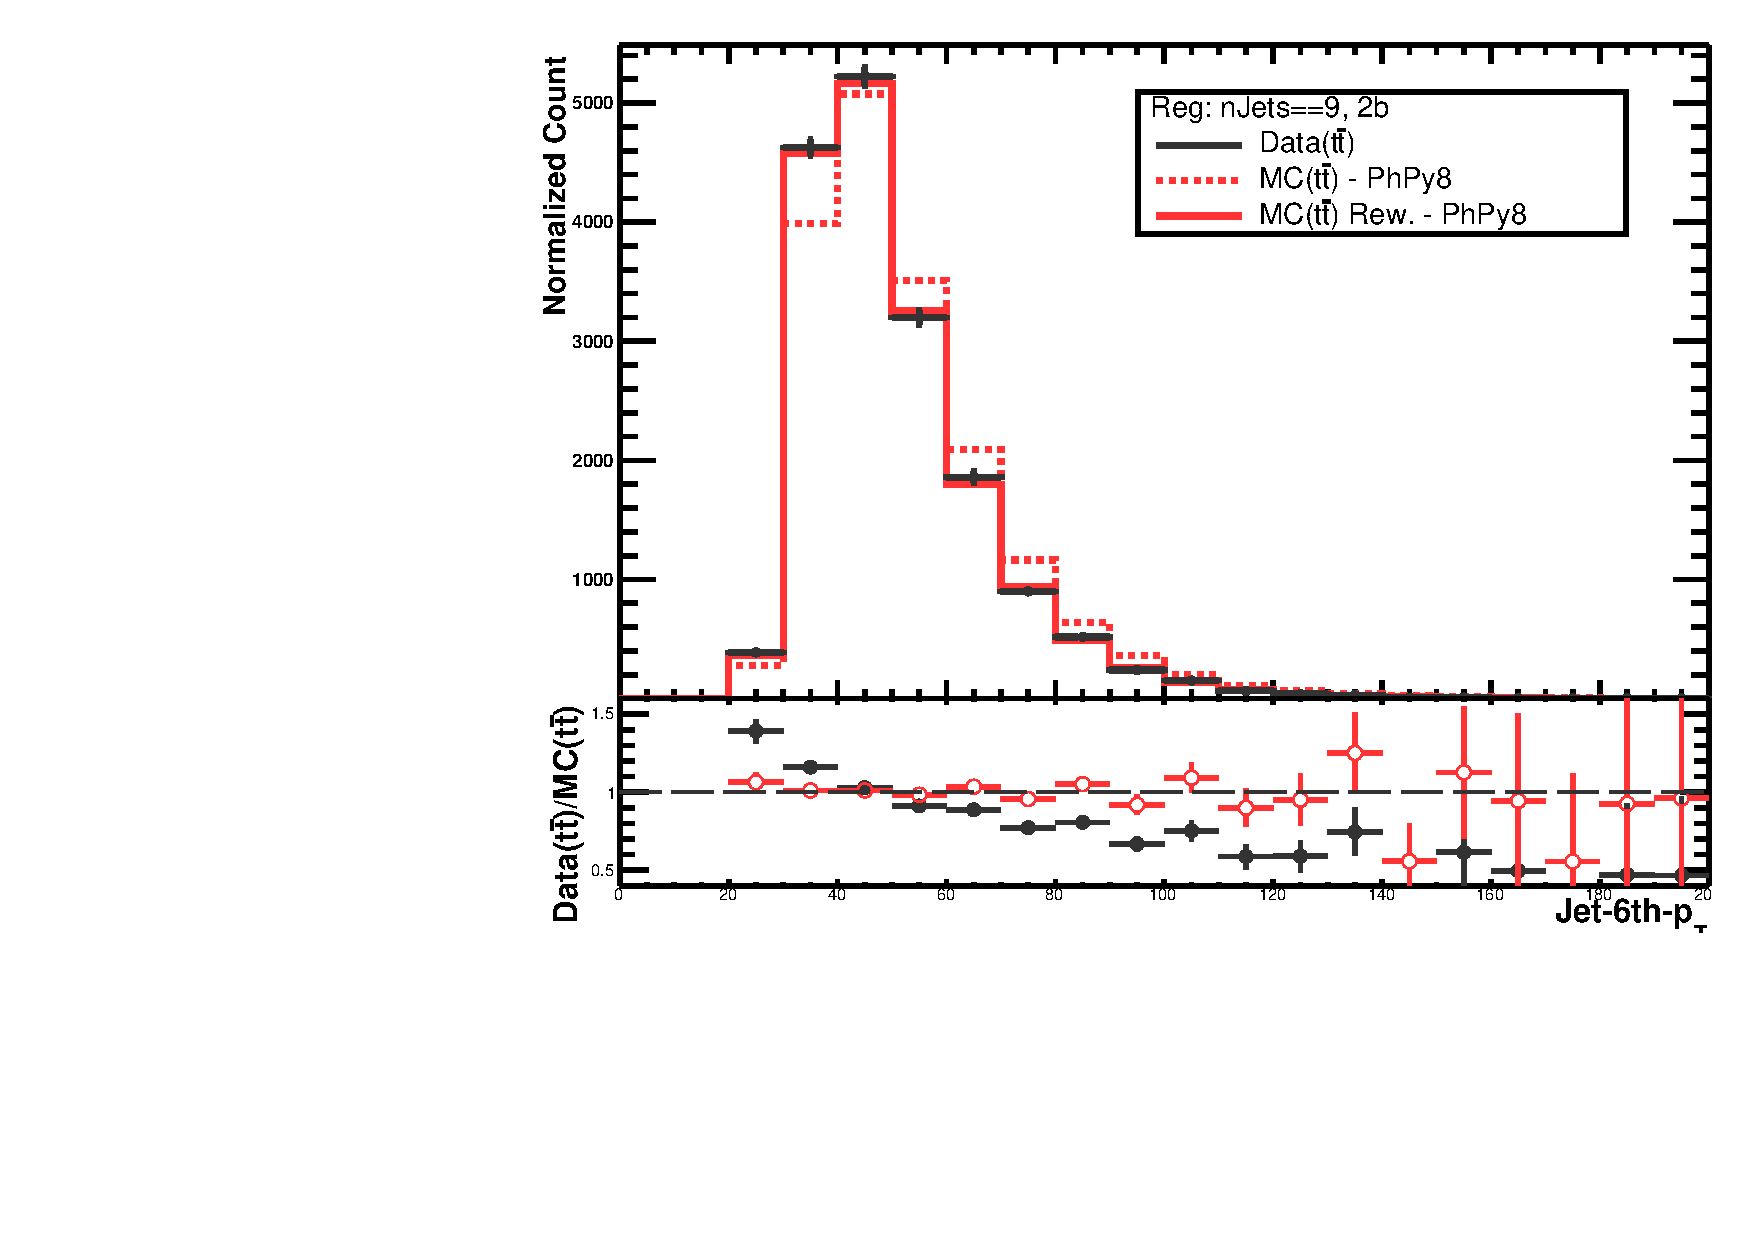
\includegraphics[width=0.24 \textwidth]{figures/rew_datamc_hfinckin_212169/1_ratiojet_pt_5__1e3_nJetsee9__1LOS.pdf} &
    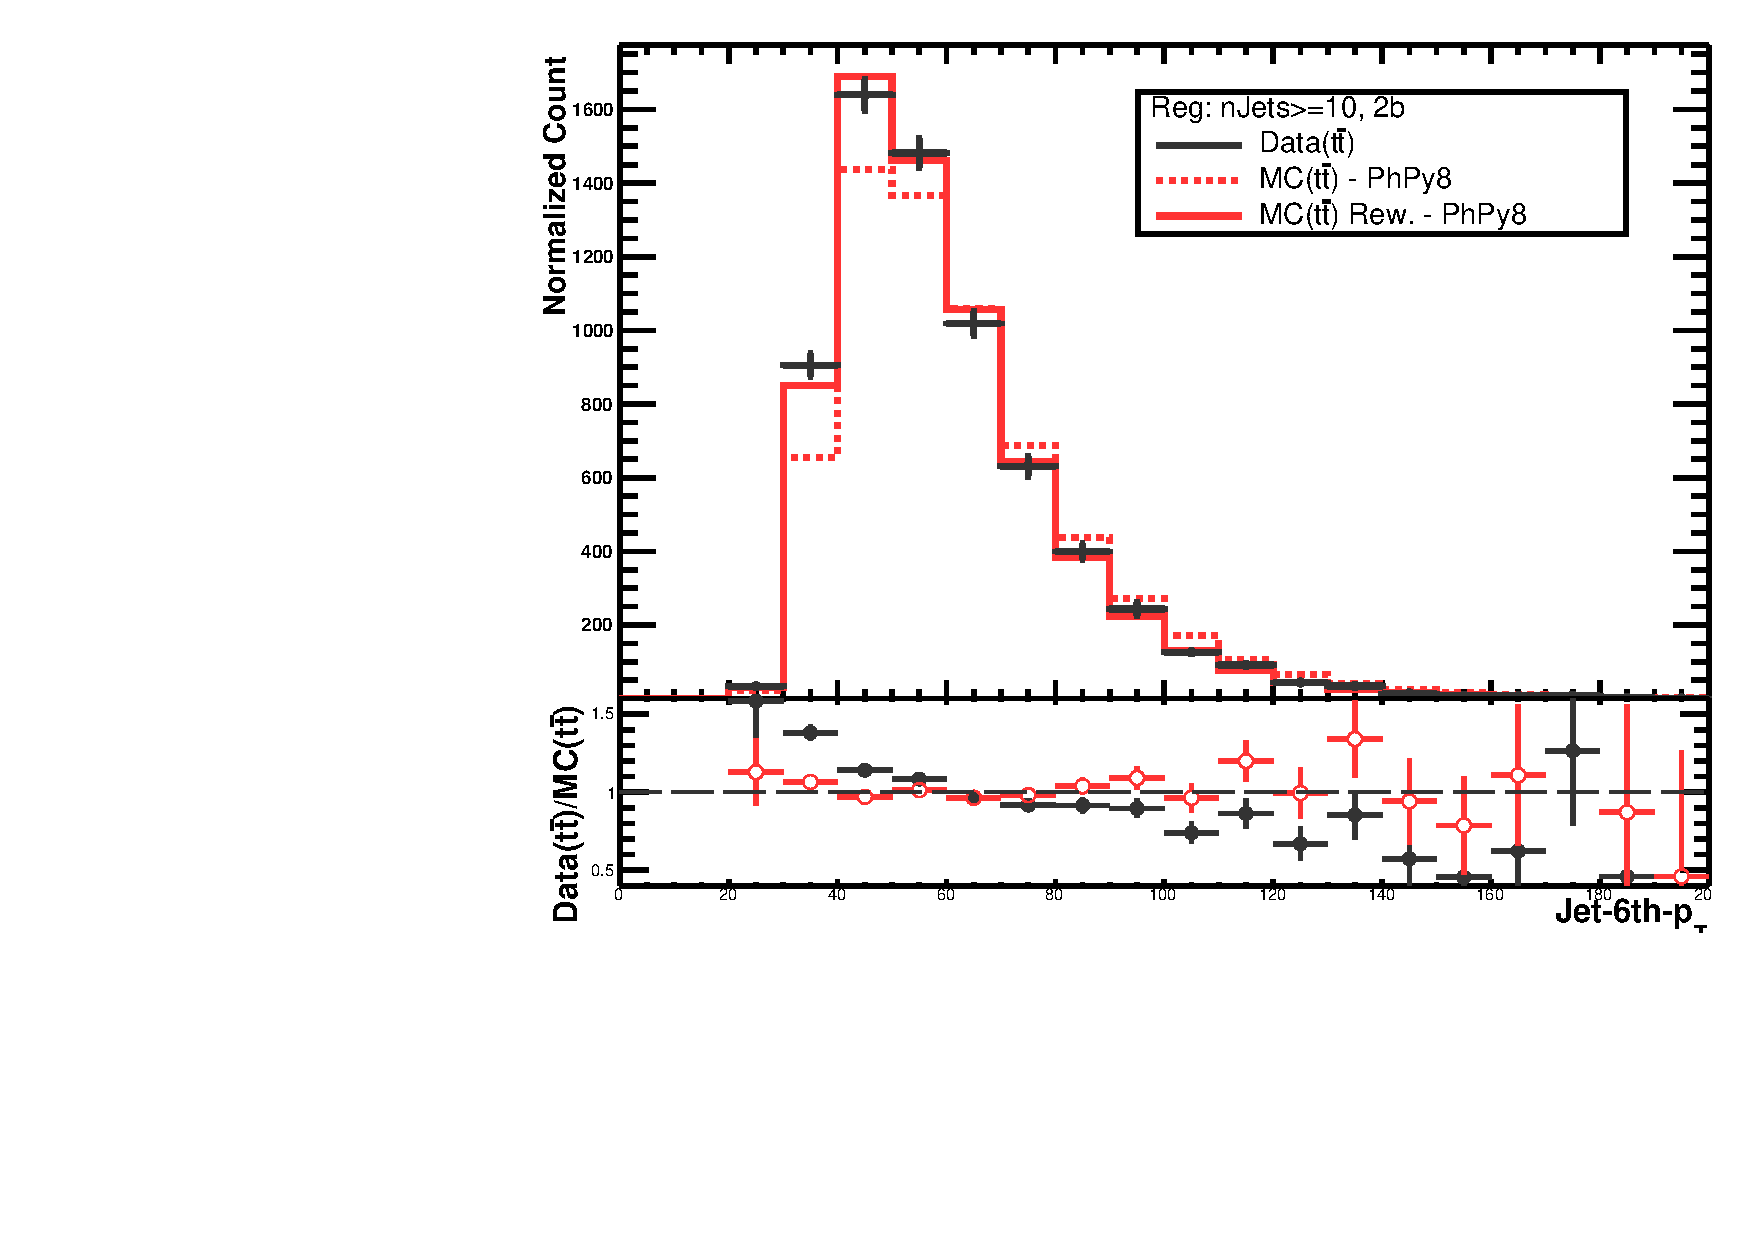
\includegraphics[width=0.24 \textwidth]{figures/rew_datamc_hfinckin_212169/1_ratiojet_pt_5__1e3_nJetsge10__1LOS.pdf} \\
    \end{tabular}
    
\end{center}
\end{figure}

\begin{figure}[htbp!]
    \begin{center} \setlength{\tabcolsep}{2.5pt}\footnotesize
    \begin{tabular}{cccc}
    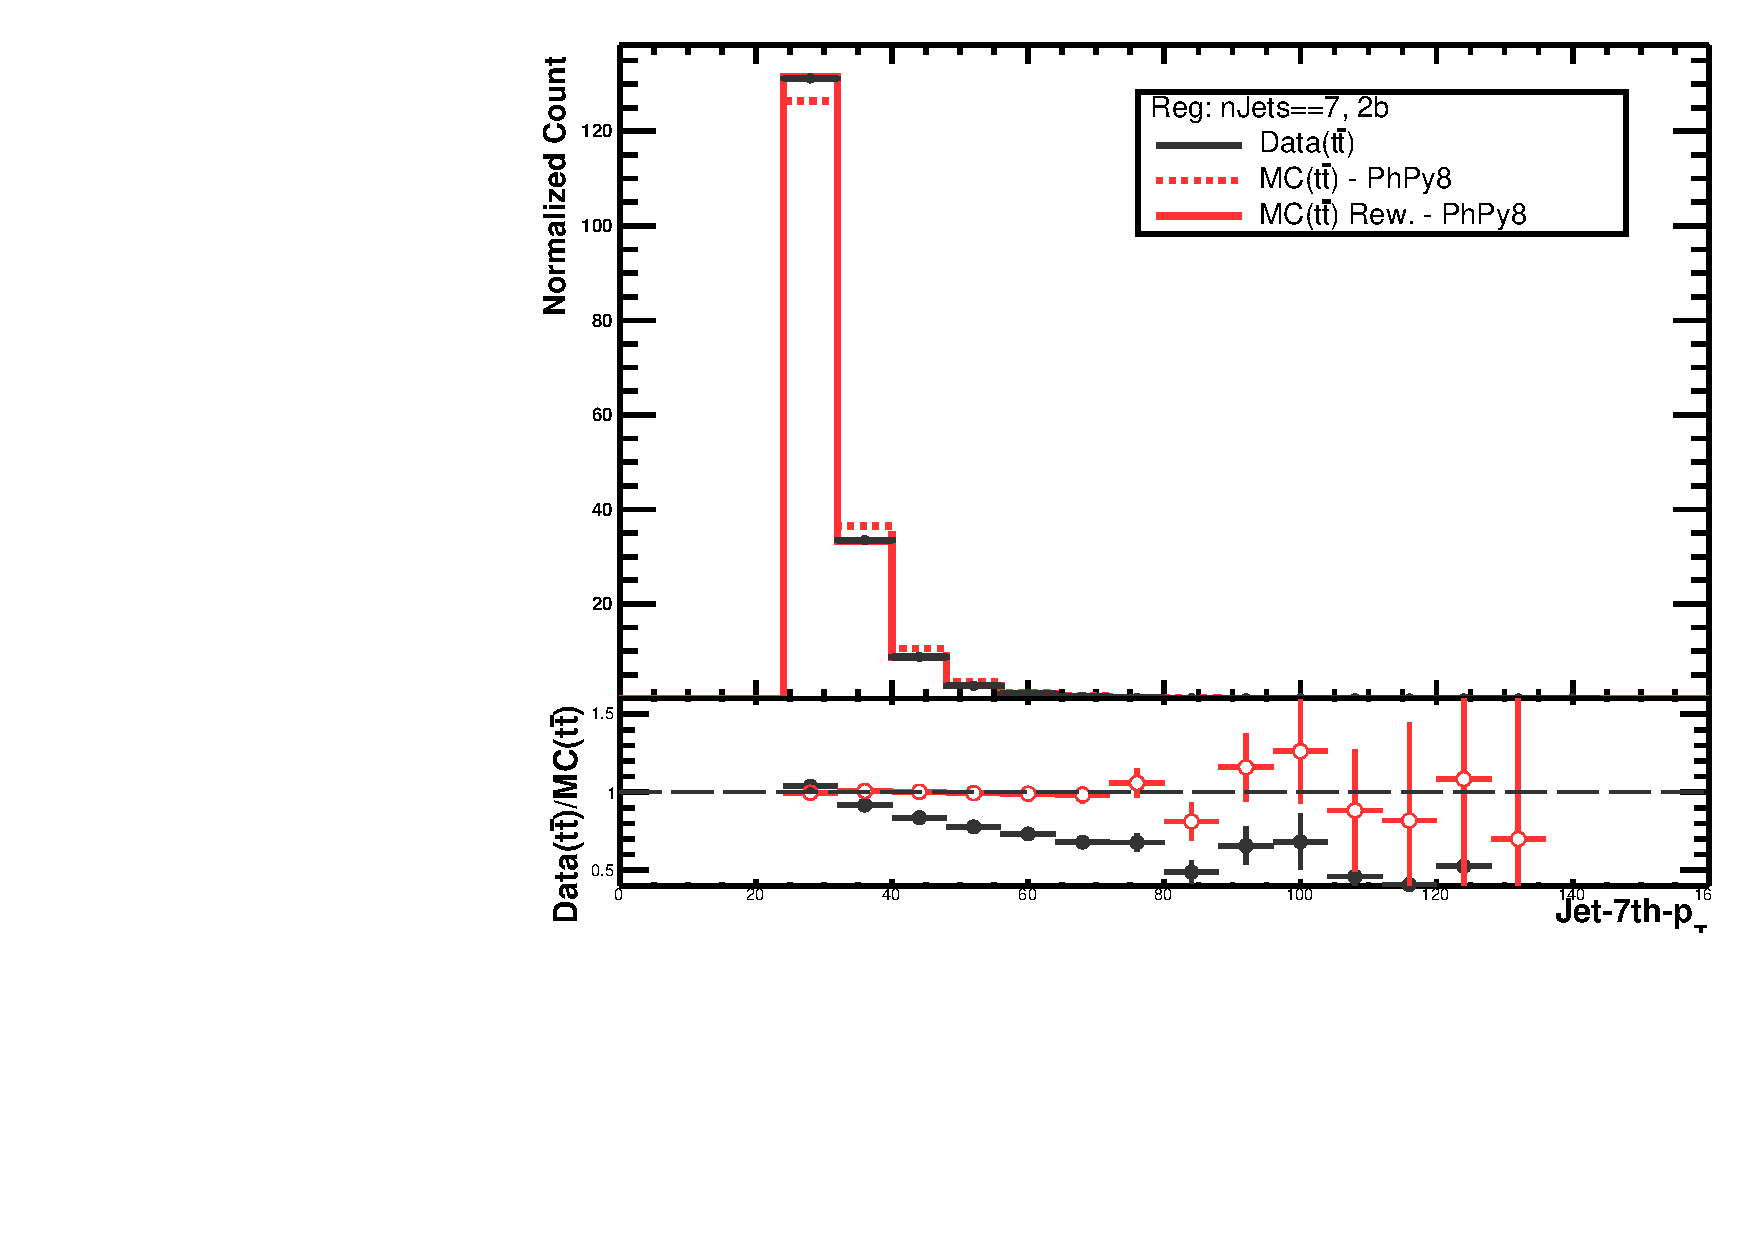
\includegraphics[width=0.24 \textwidth]{figures/rew_datamc_hfinckin_212169/1_ratiojet_pt_6__1e3_nJetsee7__1LOS.pdf} &
    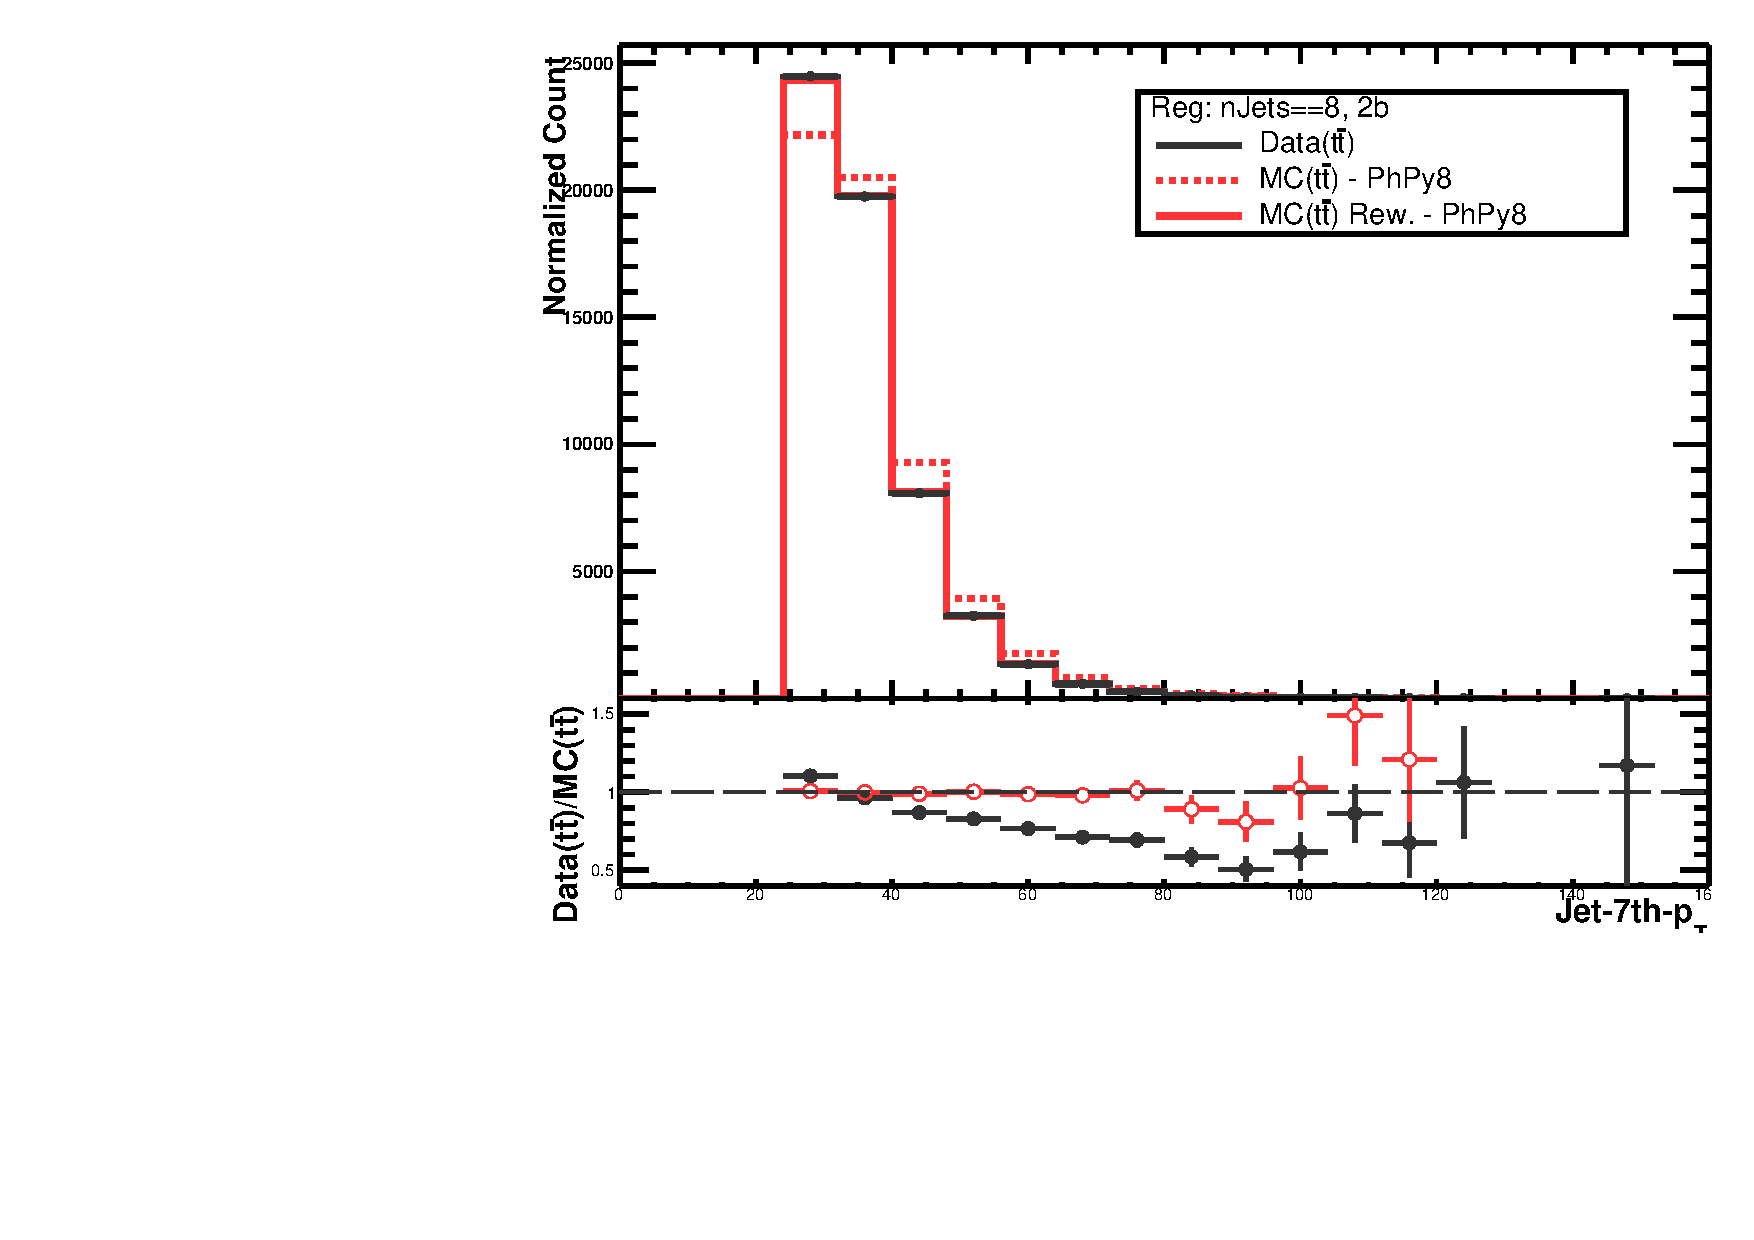
\includegraphics[width=0.24 \textwidth]{figures/rew_datamc_hfinckin_212169/1_ratiojet_pt_6__1e3_nJetsee8__1LOS.pdf} &
    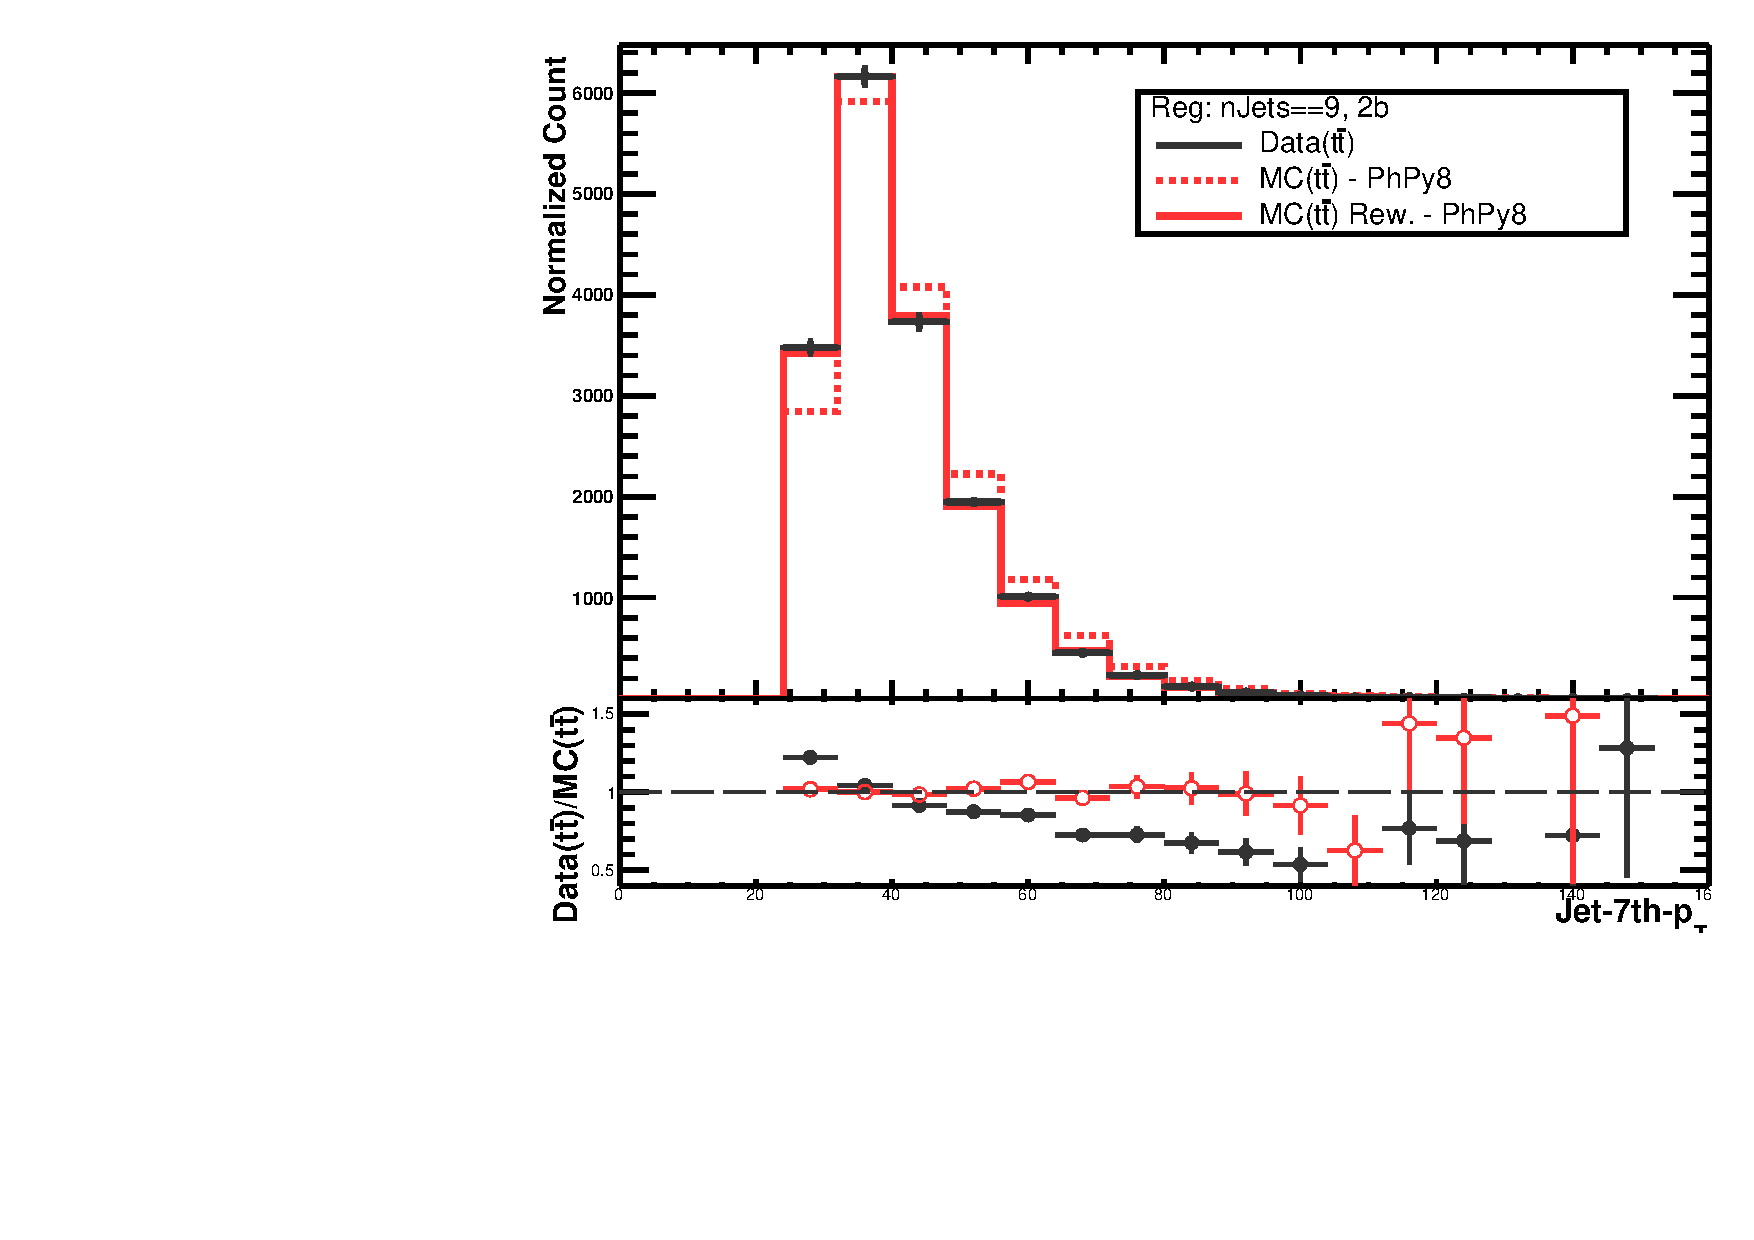
\includegraphics[width=0.24 \textwidth]{figures/rew_datamc_hfinckin_212169/1_ratiojet_pt_6__1e3_nJetsee9__1LOS.pdf} &
    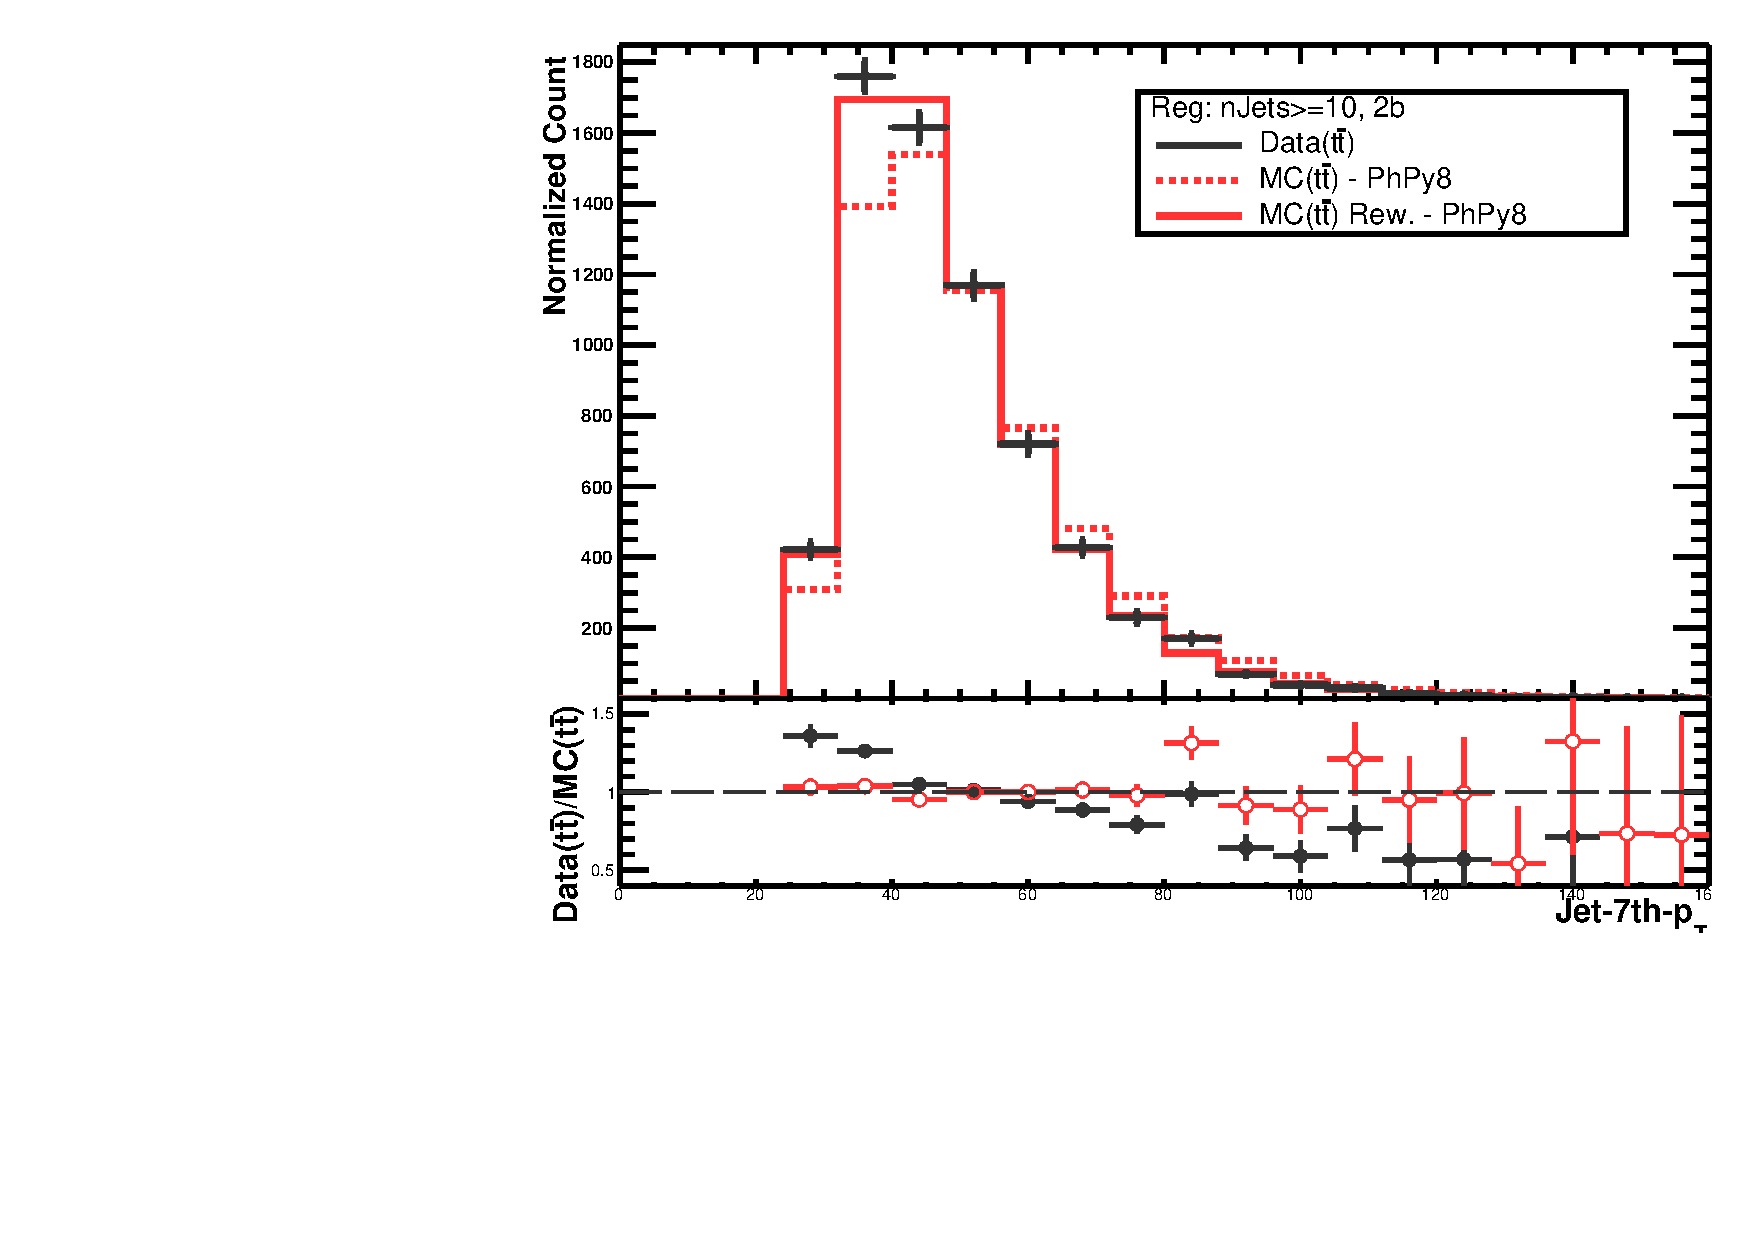
\includegraphics[width=0.24 \textwidth]{figures/rew_datamc_hfinckin_212169/1_ratiojet_pt_6__1e3_nJetsge10__1LOS.pdf} \\

    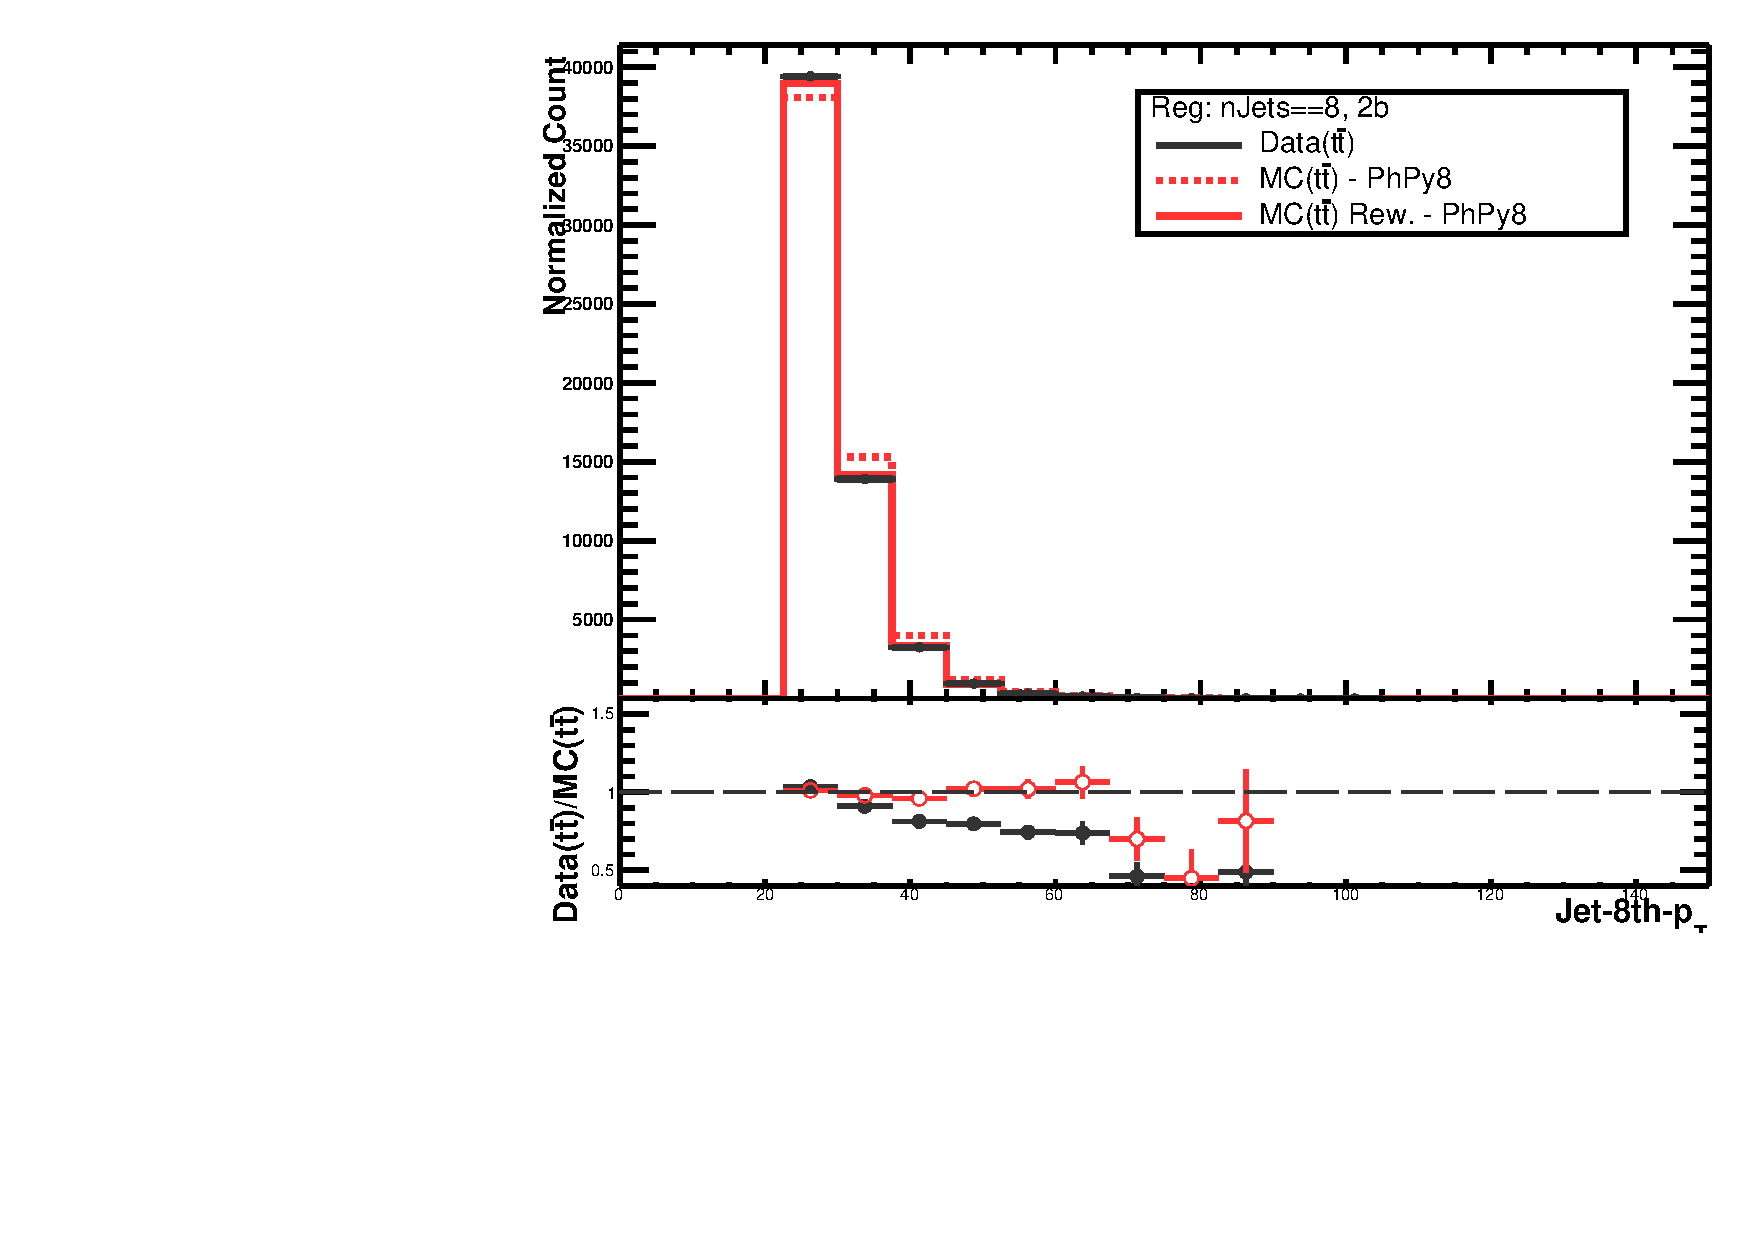
\includegraphics[width=0.24 \textwidth]{figures/rew_datamc_hfinckin_212169/1_ratioAlt__jet_pt_7__0__1e3_nJetsee8__1LOS.pdf} &
    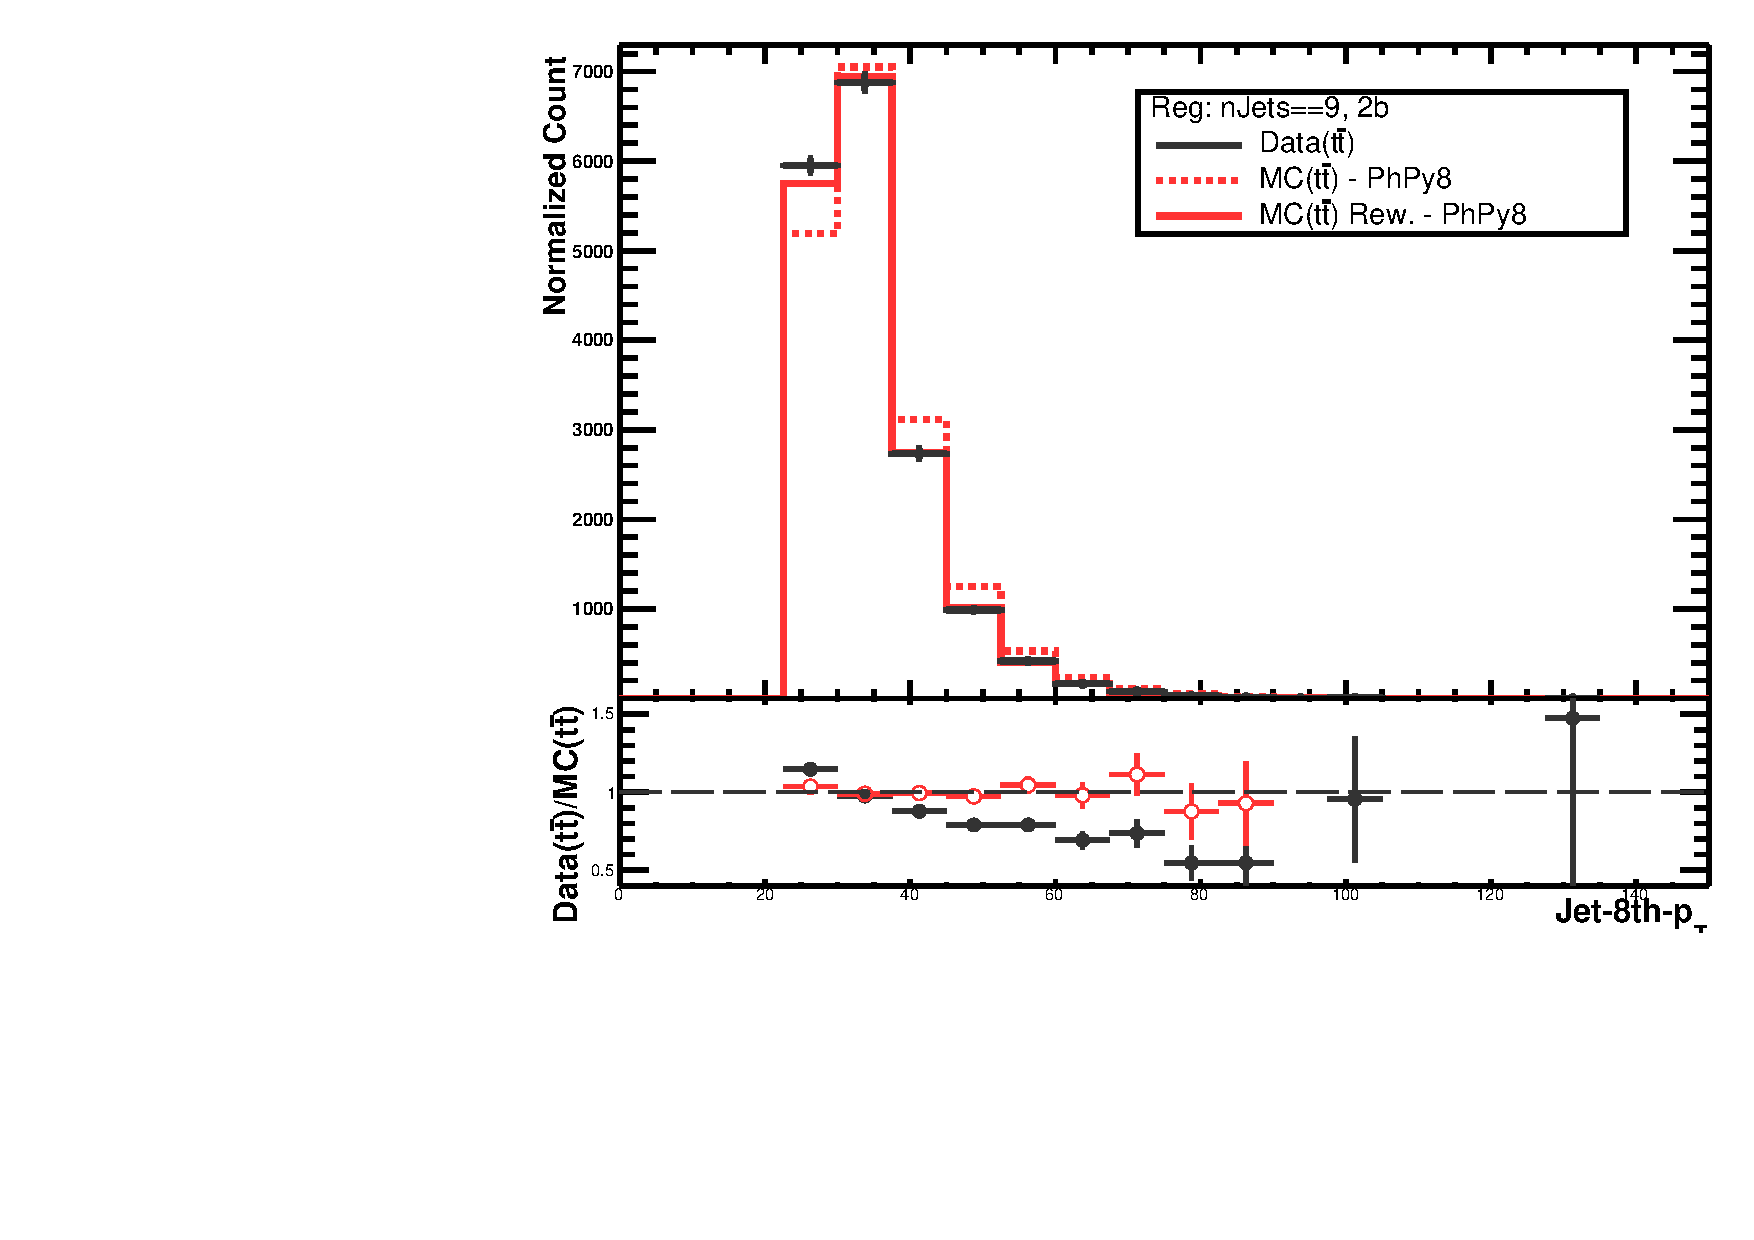
\includegraphics[width=0.24 \textwidth]{figures/rew_datamc_hfinckin_212169/1_ratioAlt__jet_pt_7__0__1e3_nJetsee9__1LOS.pdf} &
    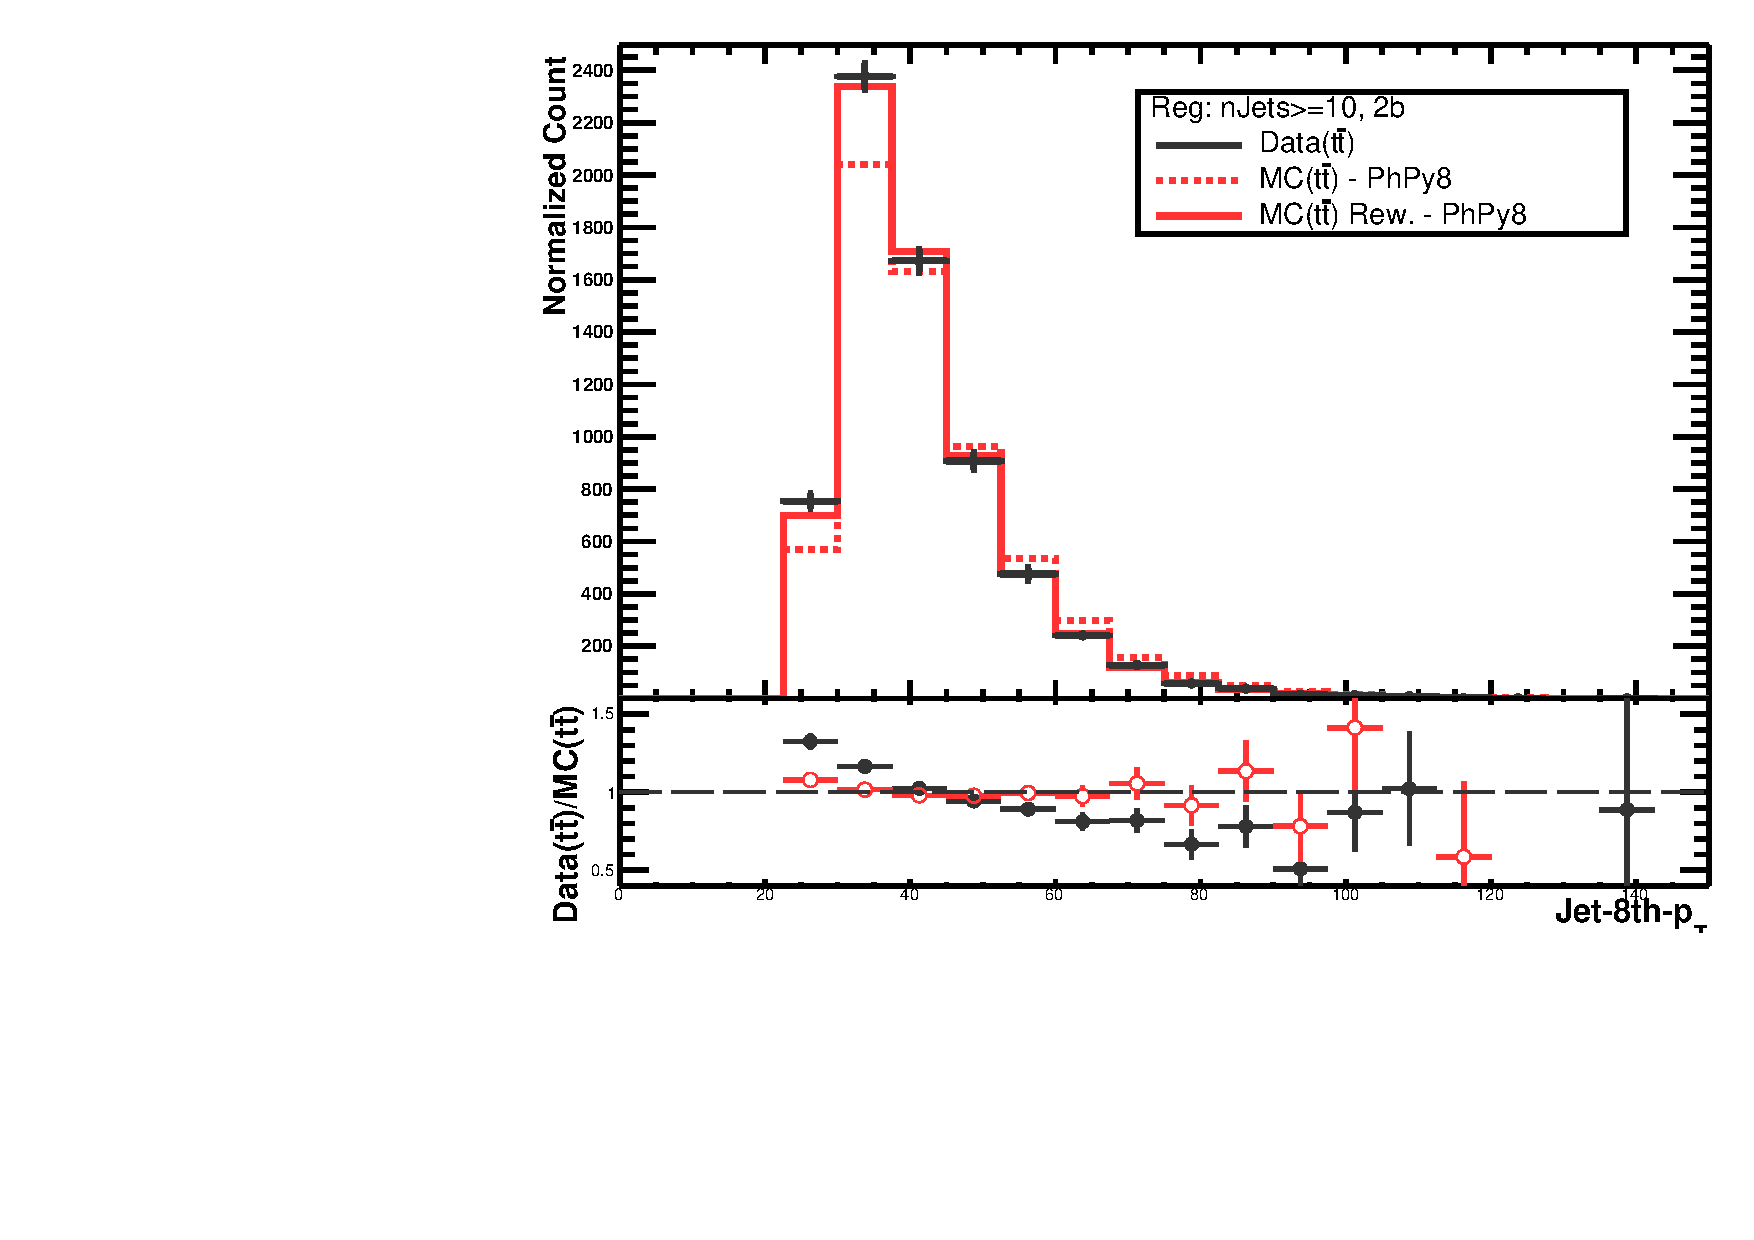
\includegraphics[width=0.24 \textwidth]{figures/rew_datamc_hfinckin_212169/1_ratioAlt__jet_pt_7__0__1e3_nJetsge10__1LOS.pdf} &
    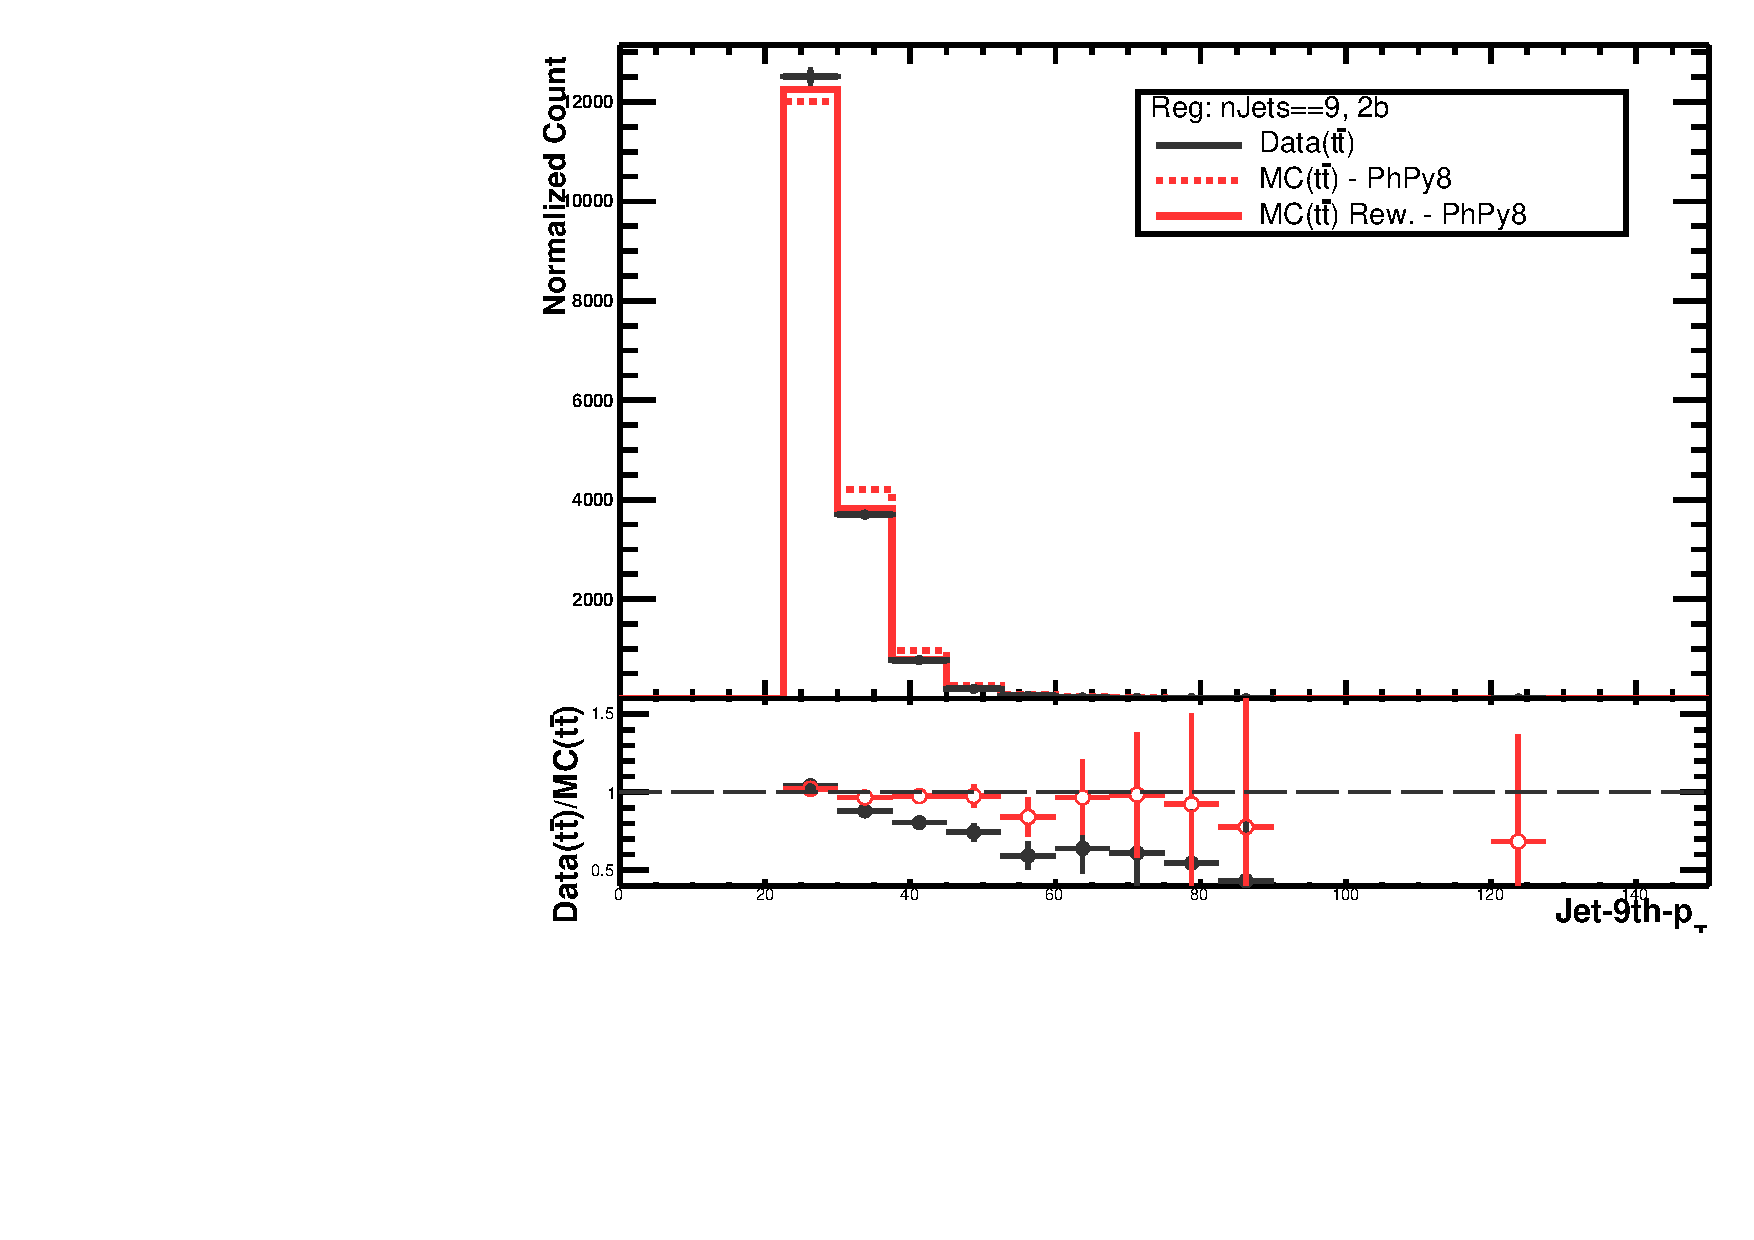
\includegraphics[width=0.24 \textwidth]{figures/rew_datamc_hfinckin_212169/1_ratioAlt__jet_pt_8__0__1e3_nJetsee9__1LOS.pdf} \\

    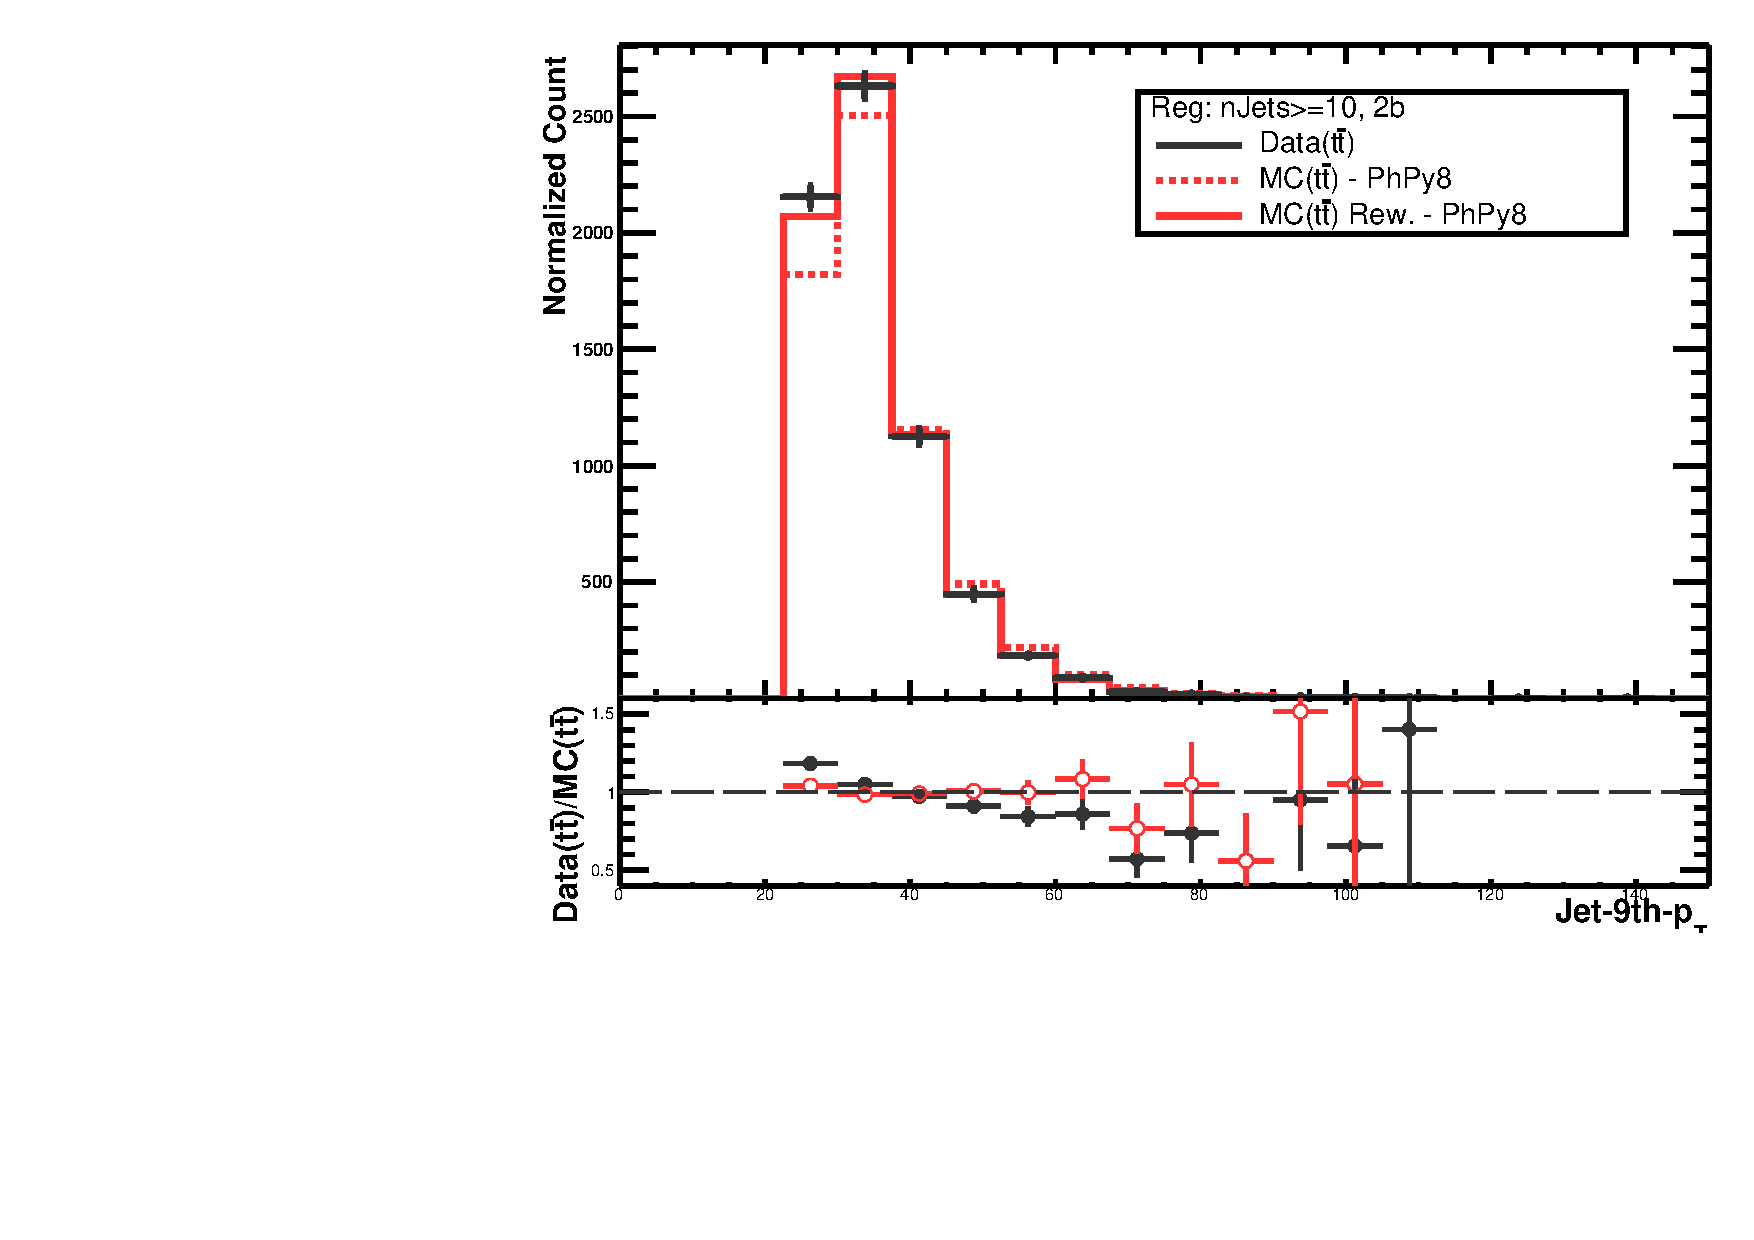
\includegraphics[width=0.24 \textwidth]{figures/rew_datamc_hfinckin_212169/1_ratioAlt__jet_pt_8__0__1e3_nJetsge10__1LOS.pdf} &
    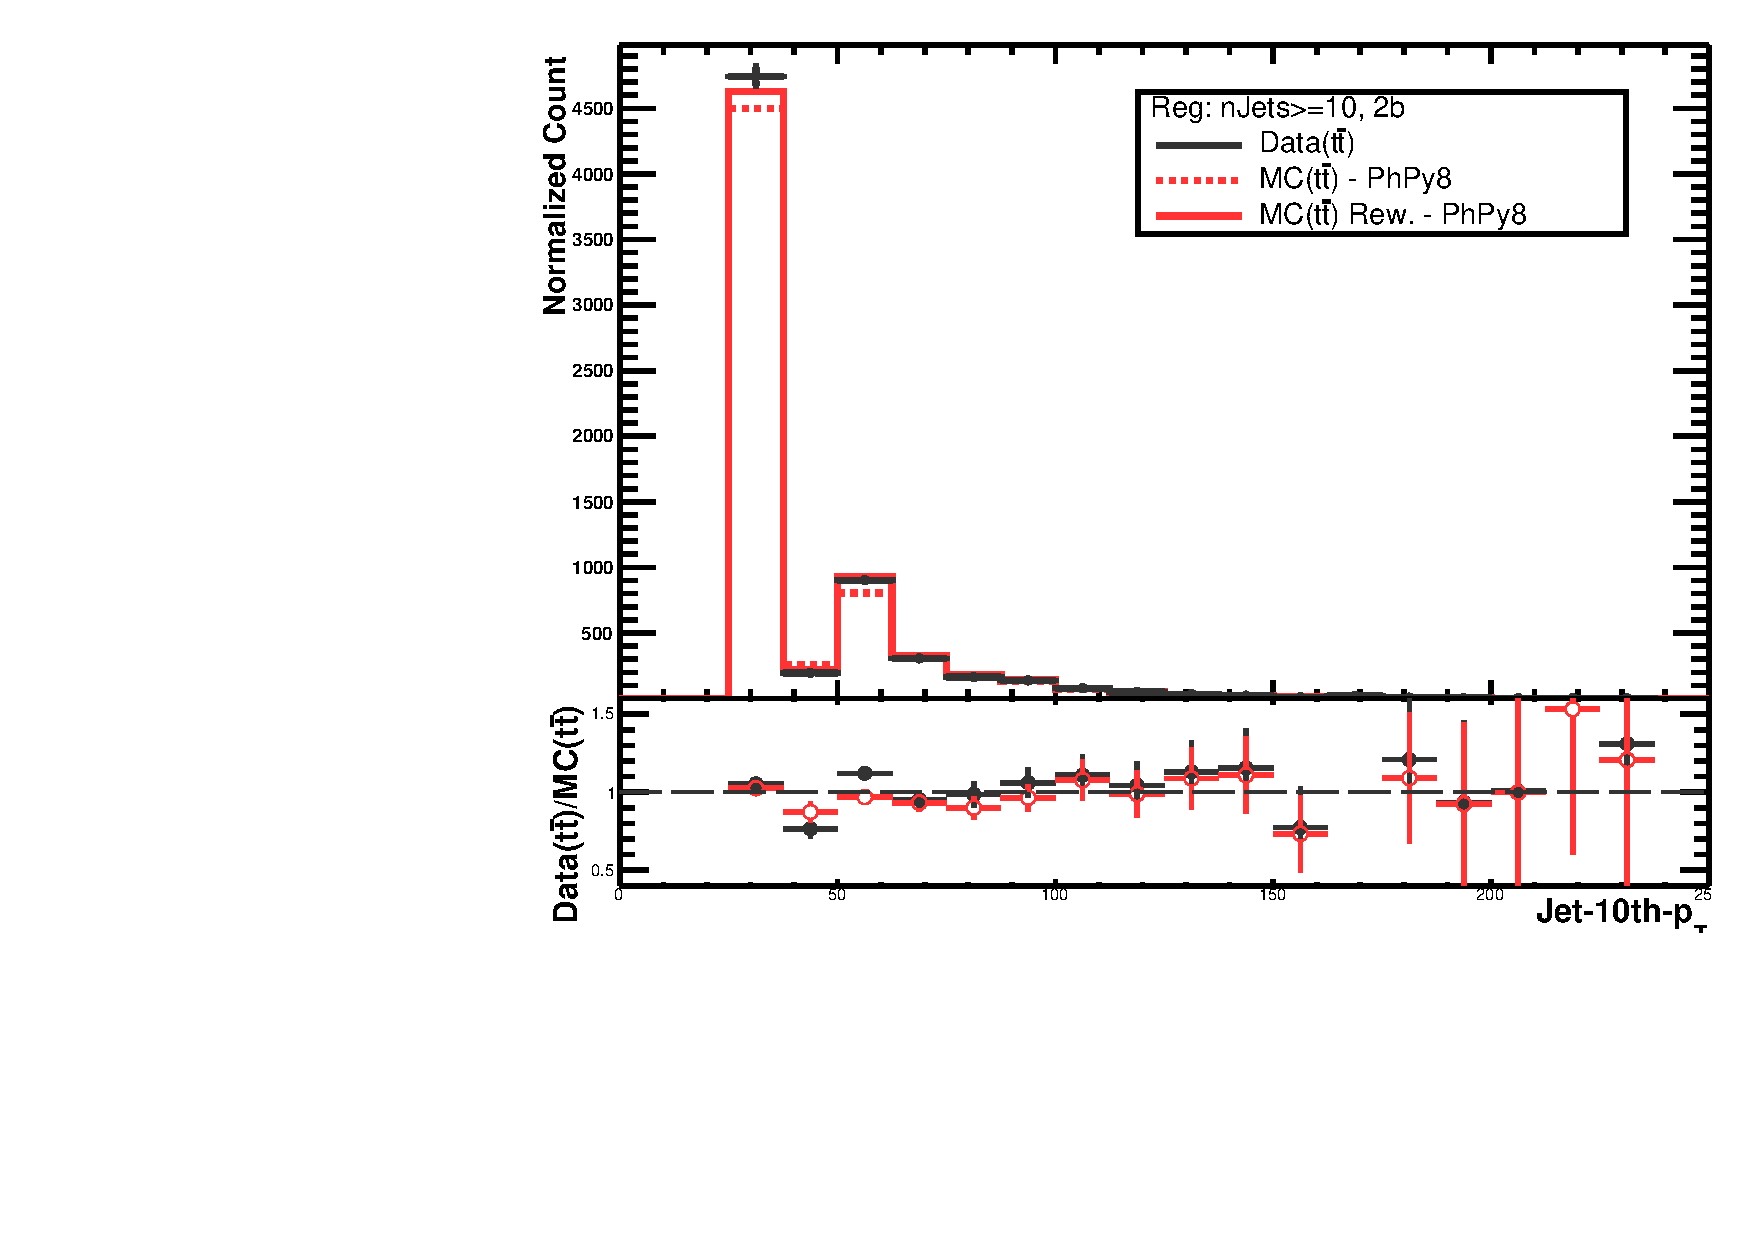
\includegraphics[width=0.24 \textwidth]{figures/rew_datamc_hfinckin_212169/1_ratioSum__jet_pt__Iteration_ge9___1e3_nJetsge10__1LOS.pdf} \\

    \end{tabular}
    \caption{\label{fig:recent_rew_1los} Some examples of NN reweighting for different features in 1L channel.}
    
\end{center}
\end{figure}

\begin{figure}[htbp!]
    \begin{center} \setlength{\tabcolsep}{2.5pt}\footnotesize
    \begin{tabular}{cccc}
    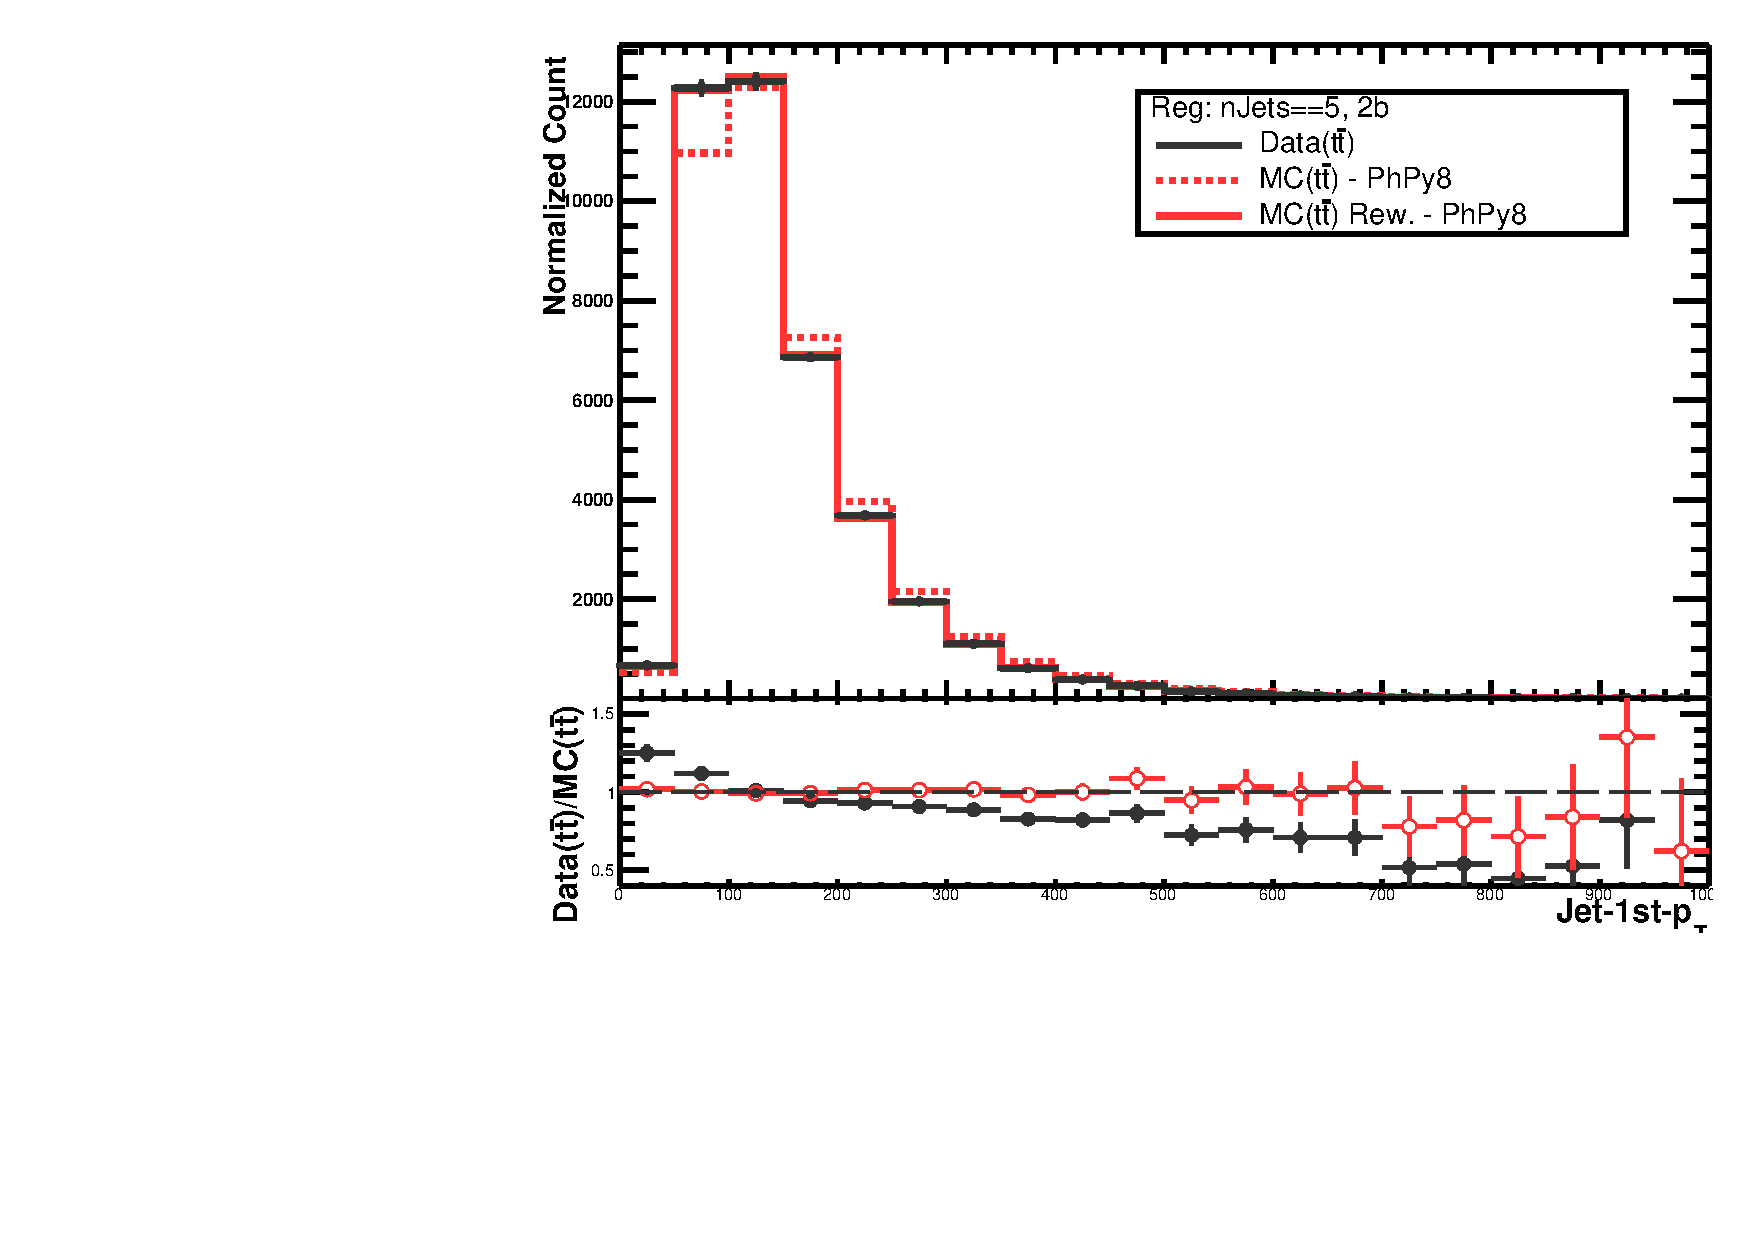
\includegraphics[width=0.24 \textwidth]{figures/rew_datamc_hfinckin_212169/1_ratiojet_pt_0__1e3_nJetsee5__2LOS.pdf} &
    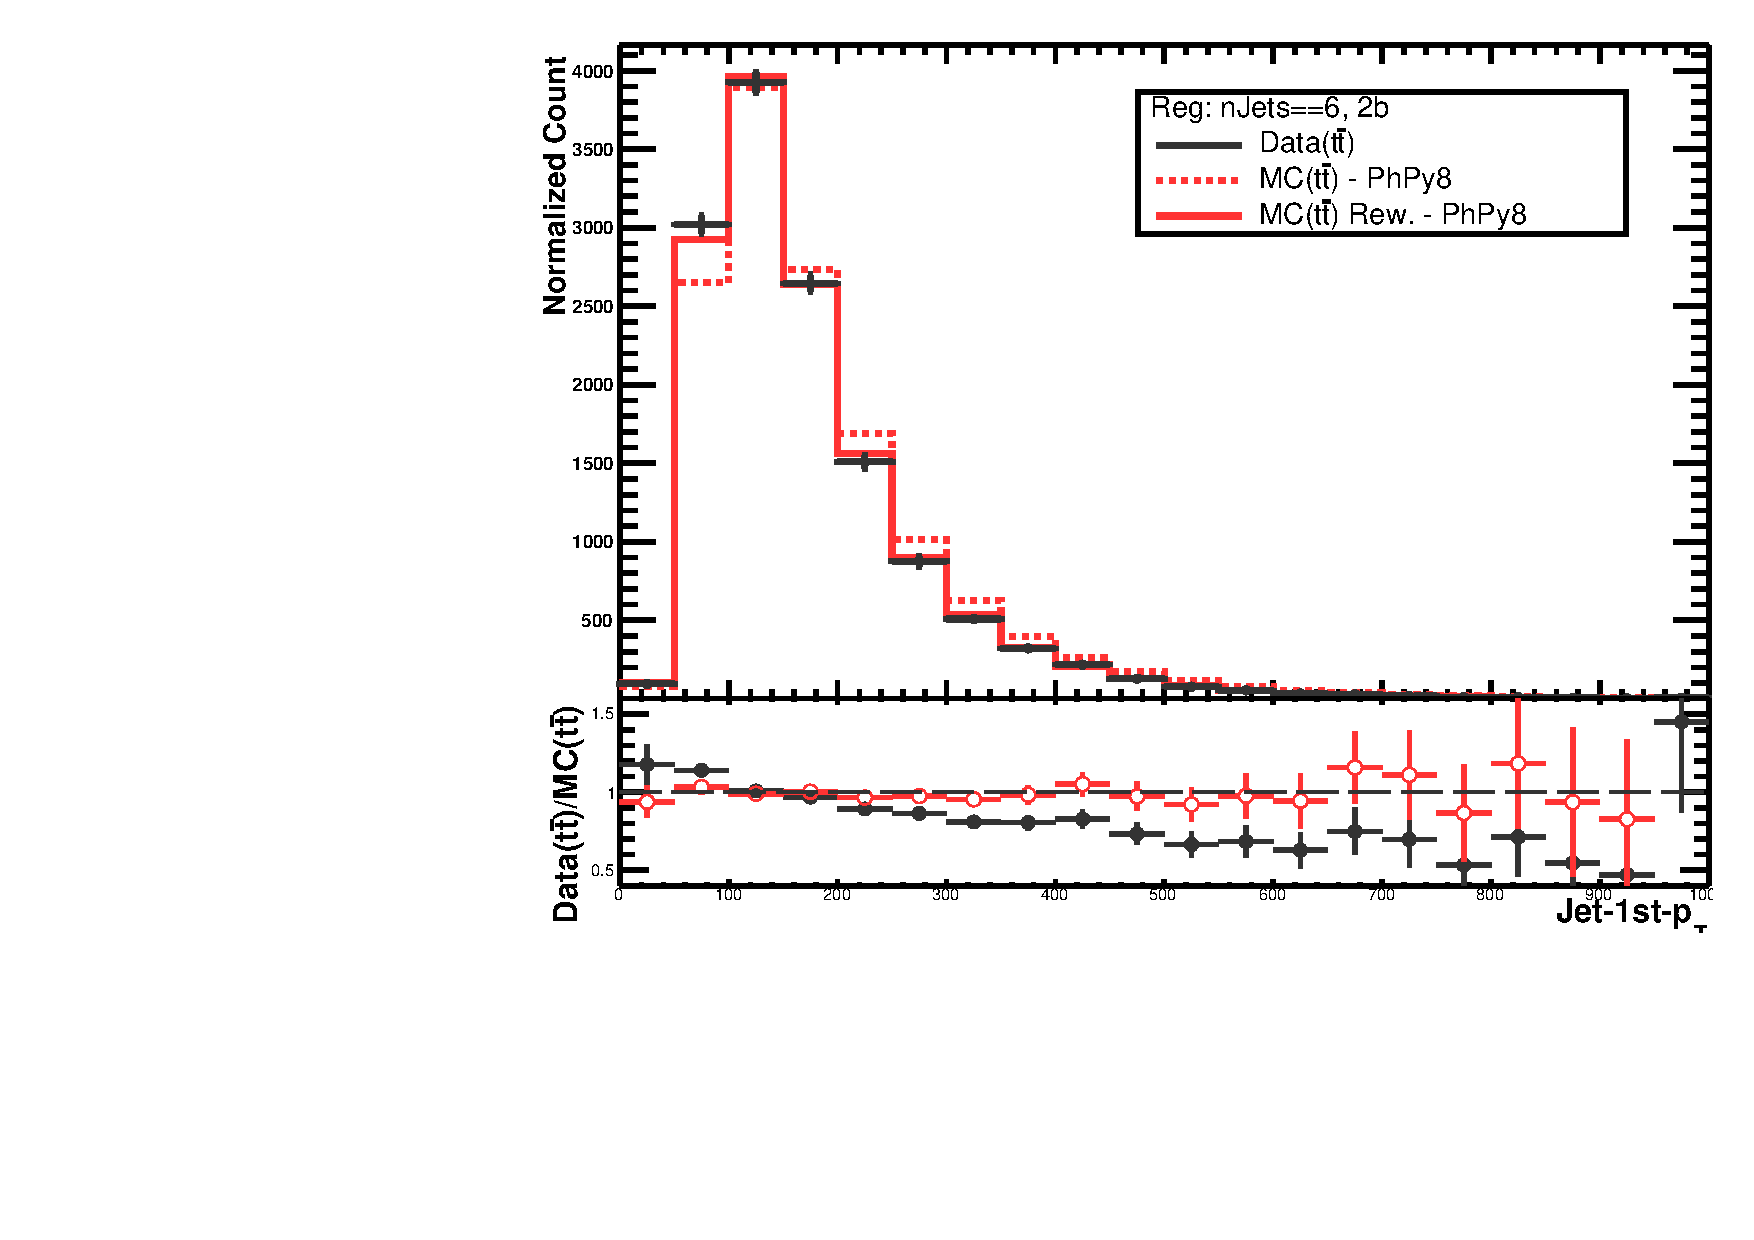
\includegraphics[width=0.24 \textwidth]{figures/rew_datamc_hfinckin_212169/1_ratiojet_pt_0__1e3_nJetsee6__2LOS.pdf} &
    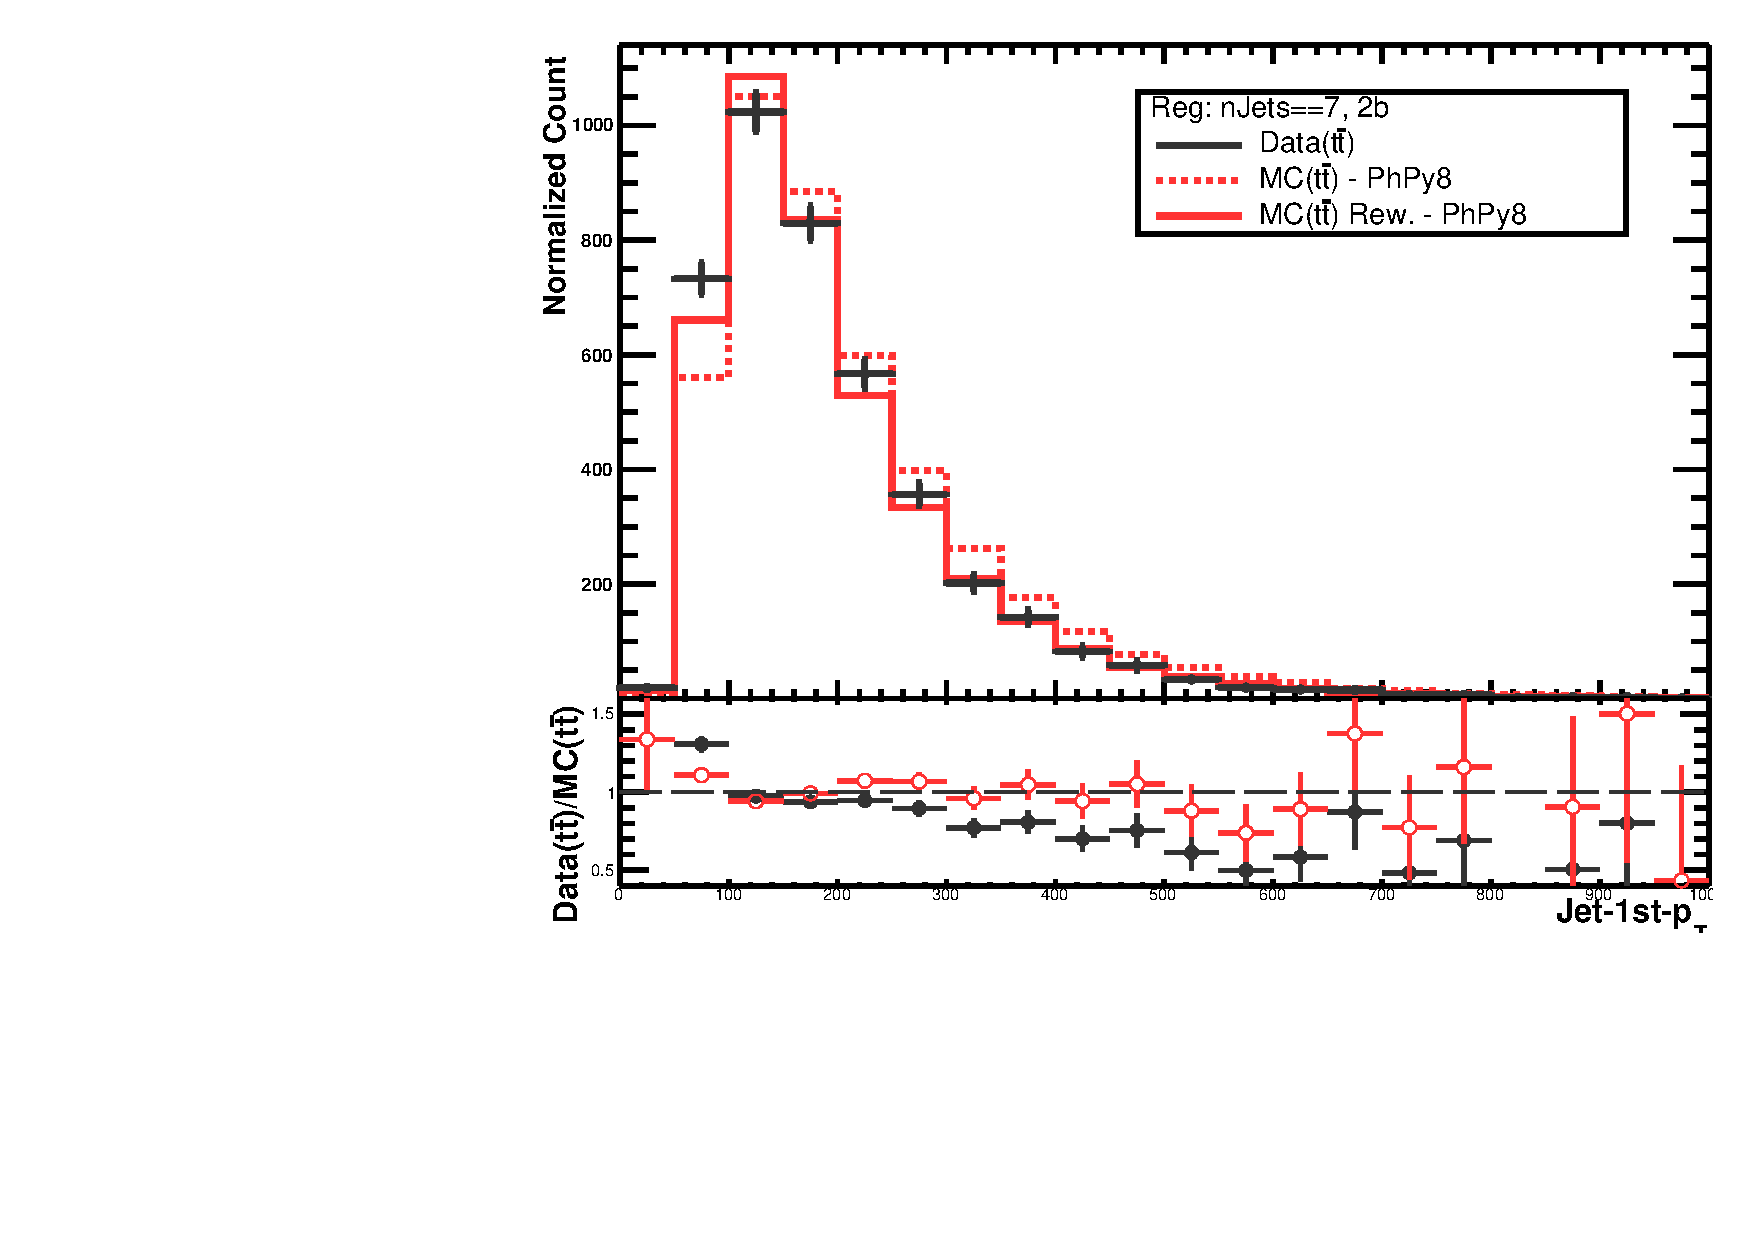
\includegraphics[width=0.24 \textwidth]{figures/rew_datamc_hfinckin_212169/1_ratiojet_pt_0__1e3_nJetsee7__2LOS.pdf} &
    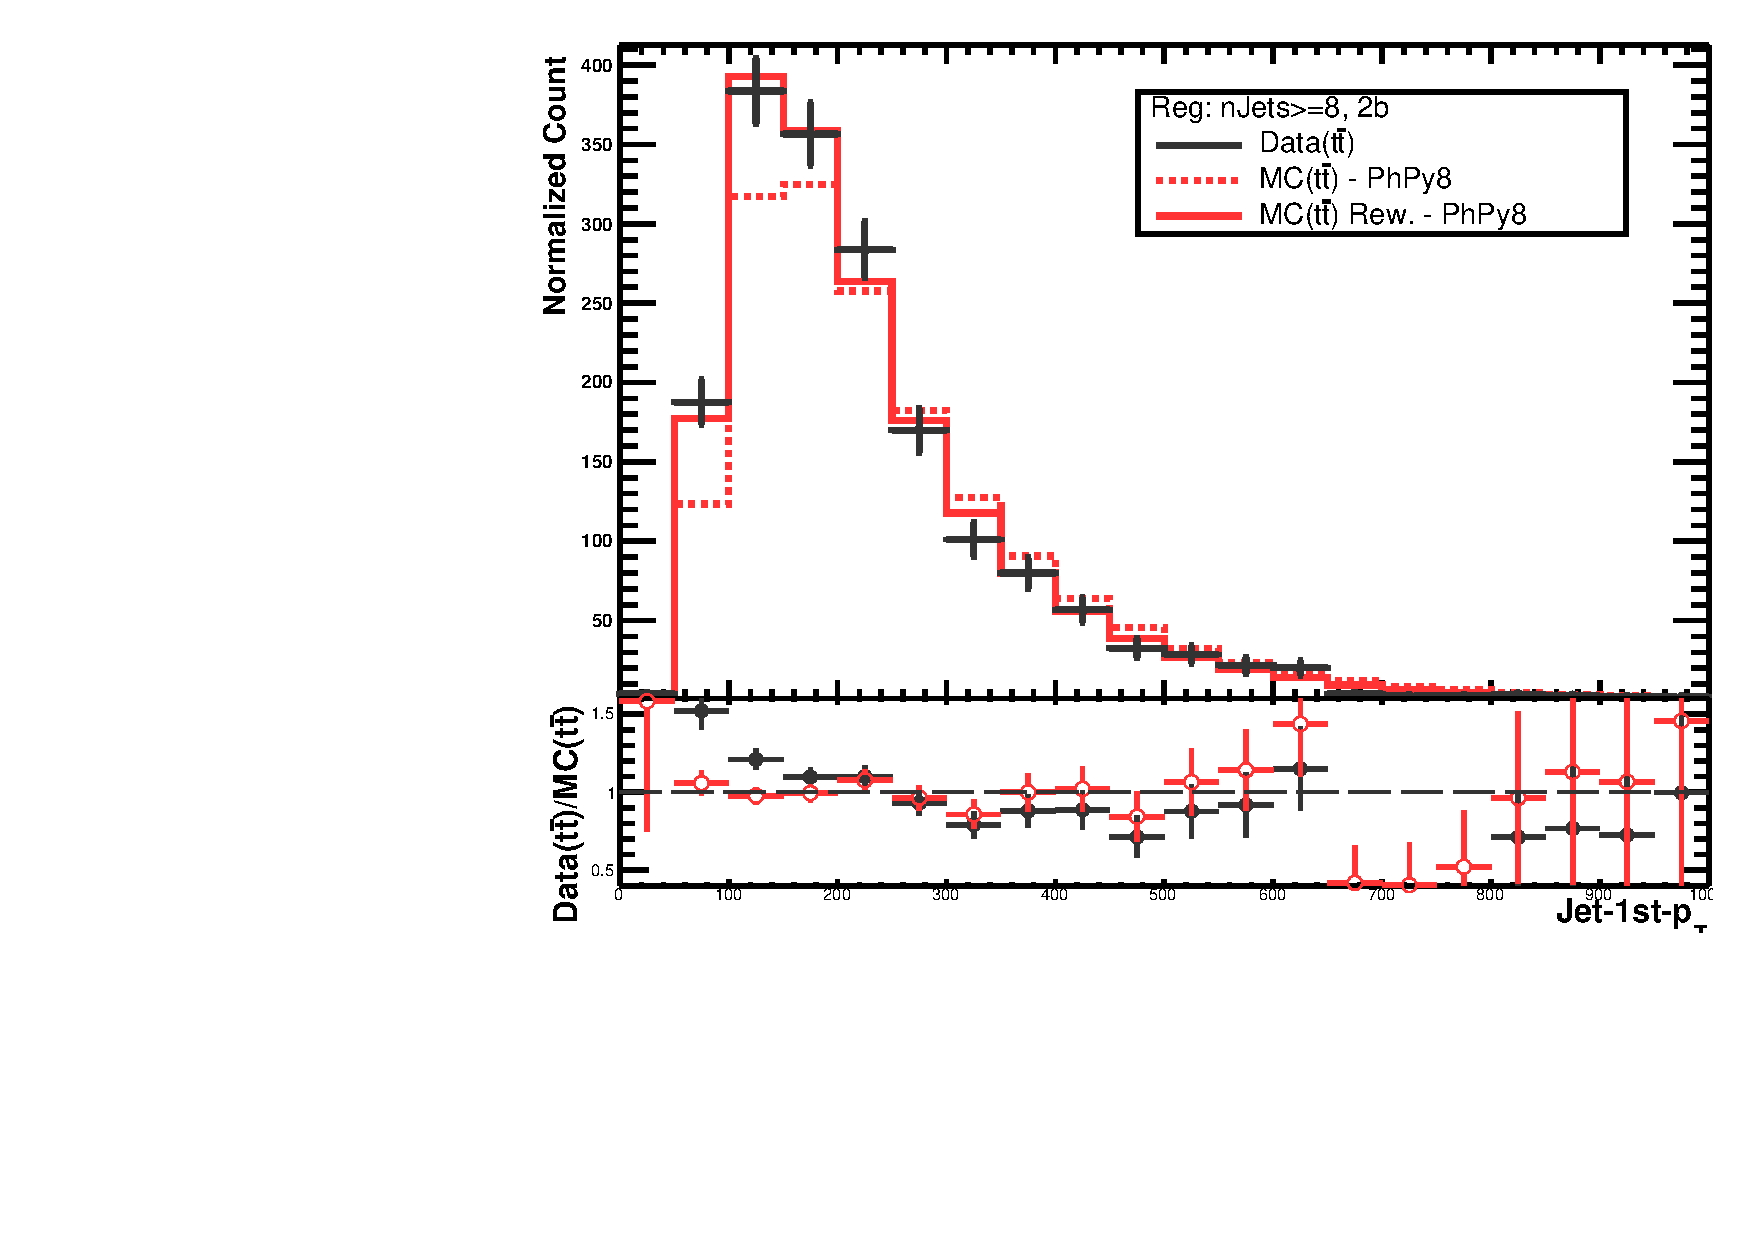
\includegraphics[width=0.24 \textwidth]{figures/rew_datamc_hfinckin_212169/1_ratiojet_pt_0__1e3_nJetsge8__2LOS.pdf} \\

    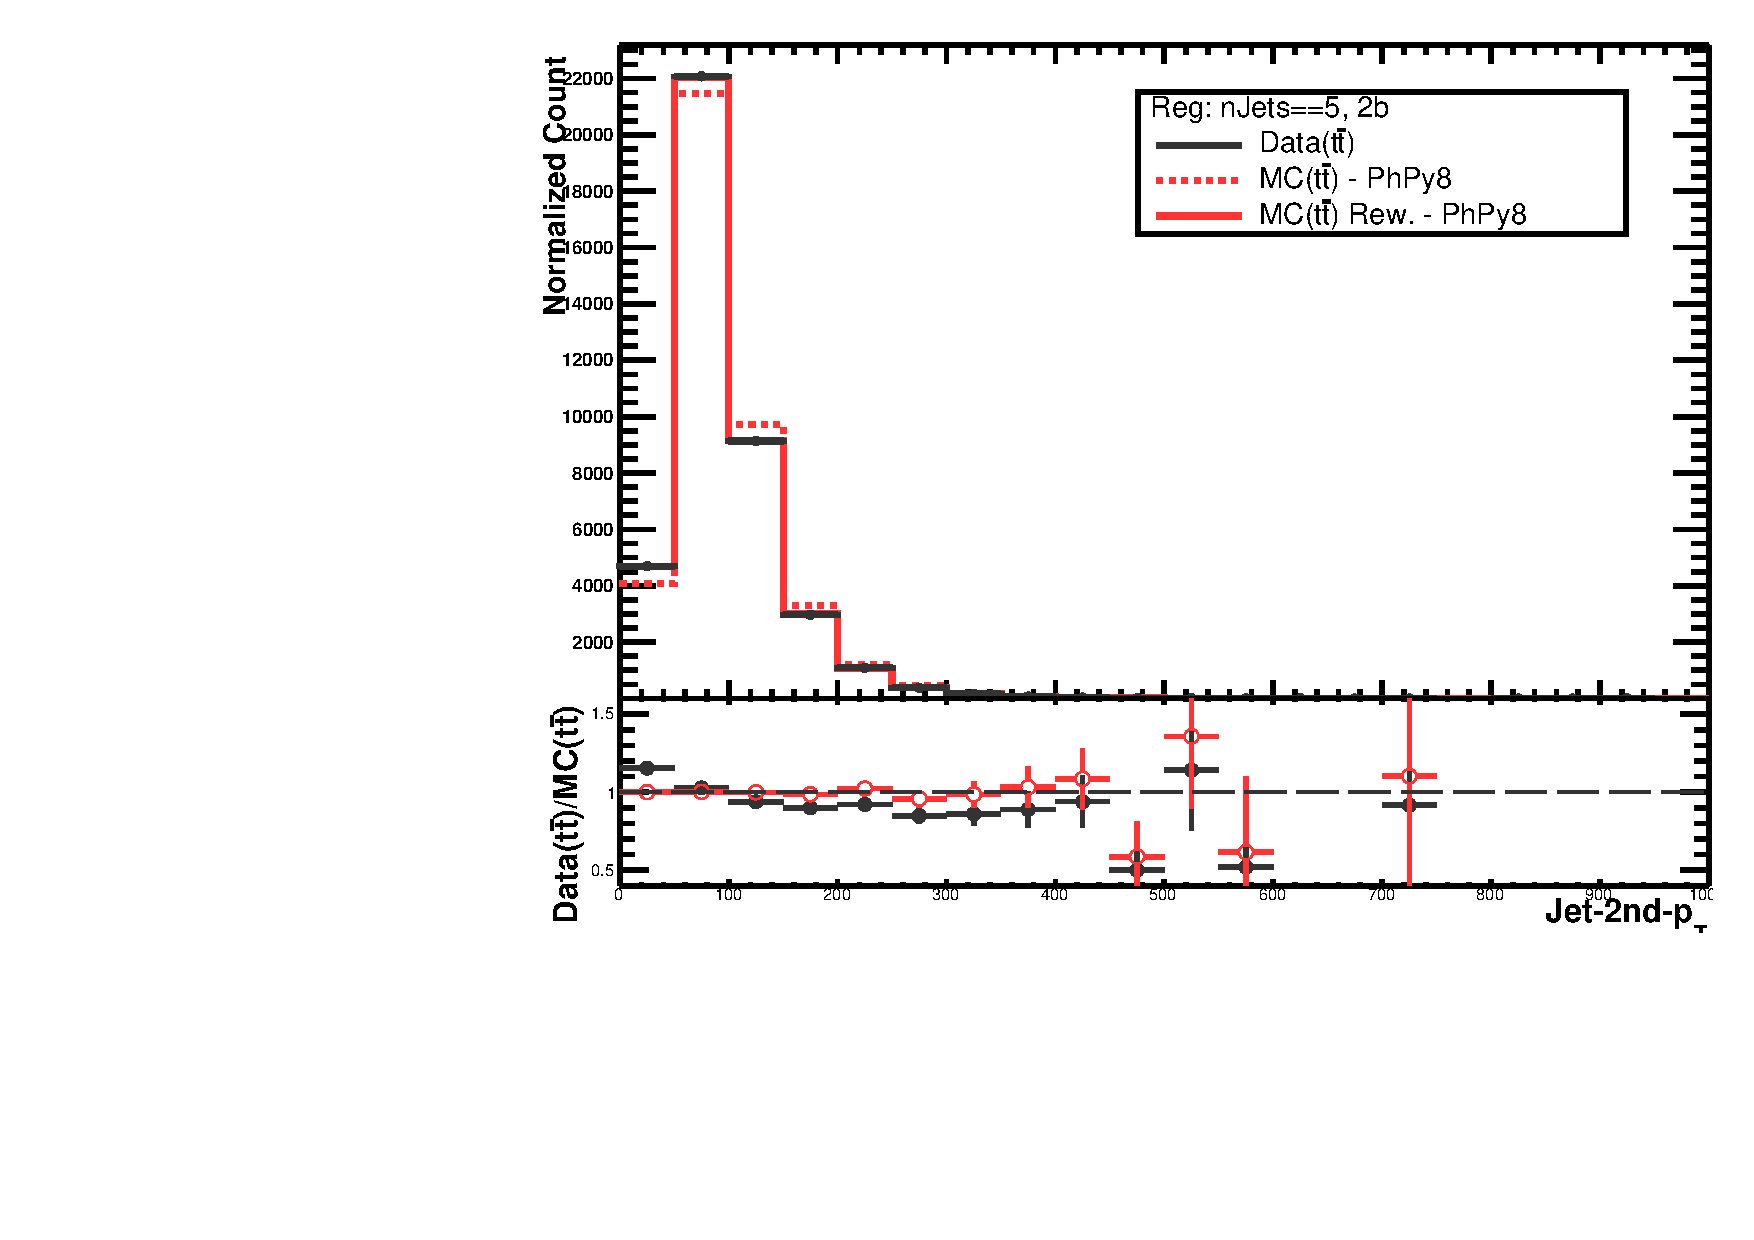
\includegraphics[width=0.24 \textwidth]{figures/rew_datamc_hfinckin_212169/1_ratiojet_pt_1__1e3_nJetsee5__2LOS.pdf} &
    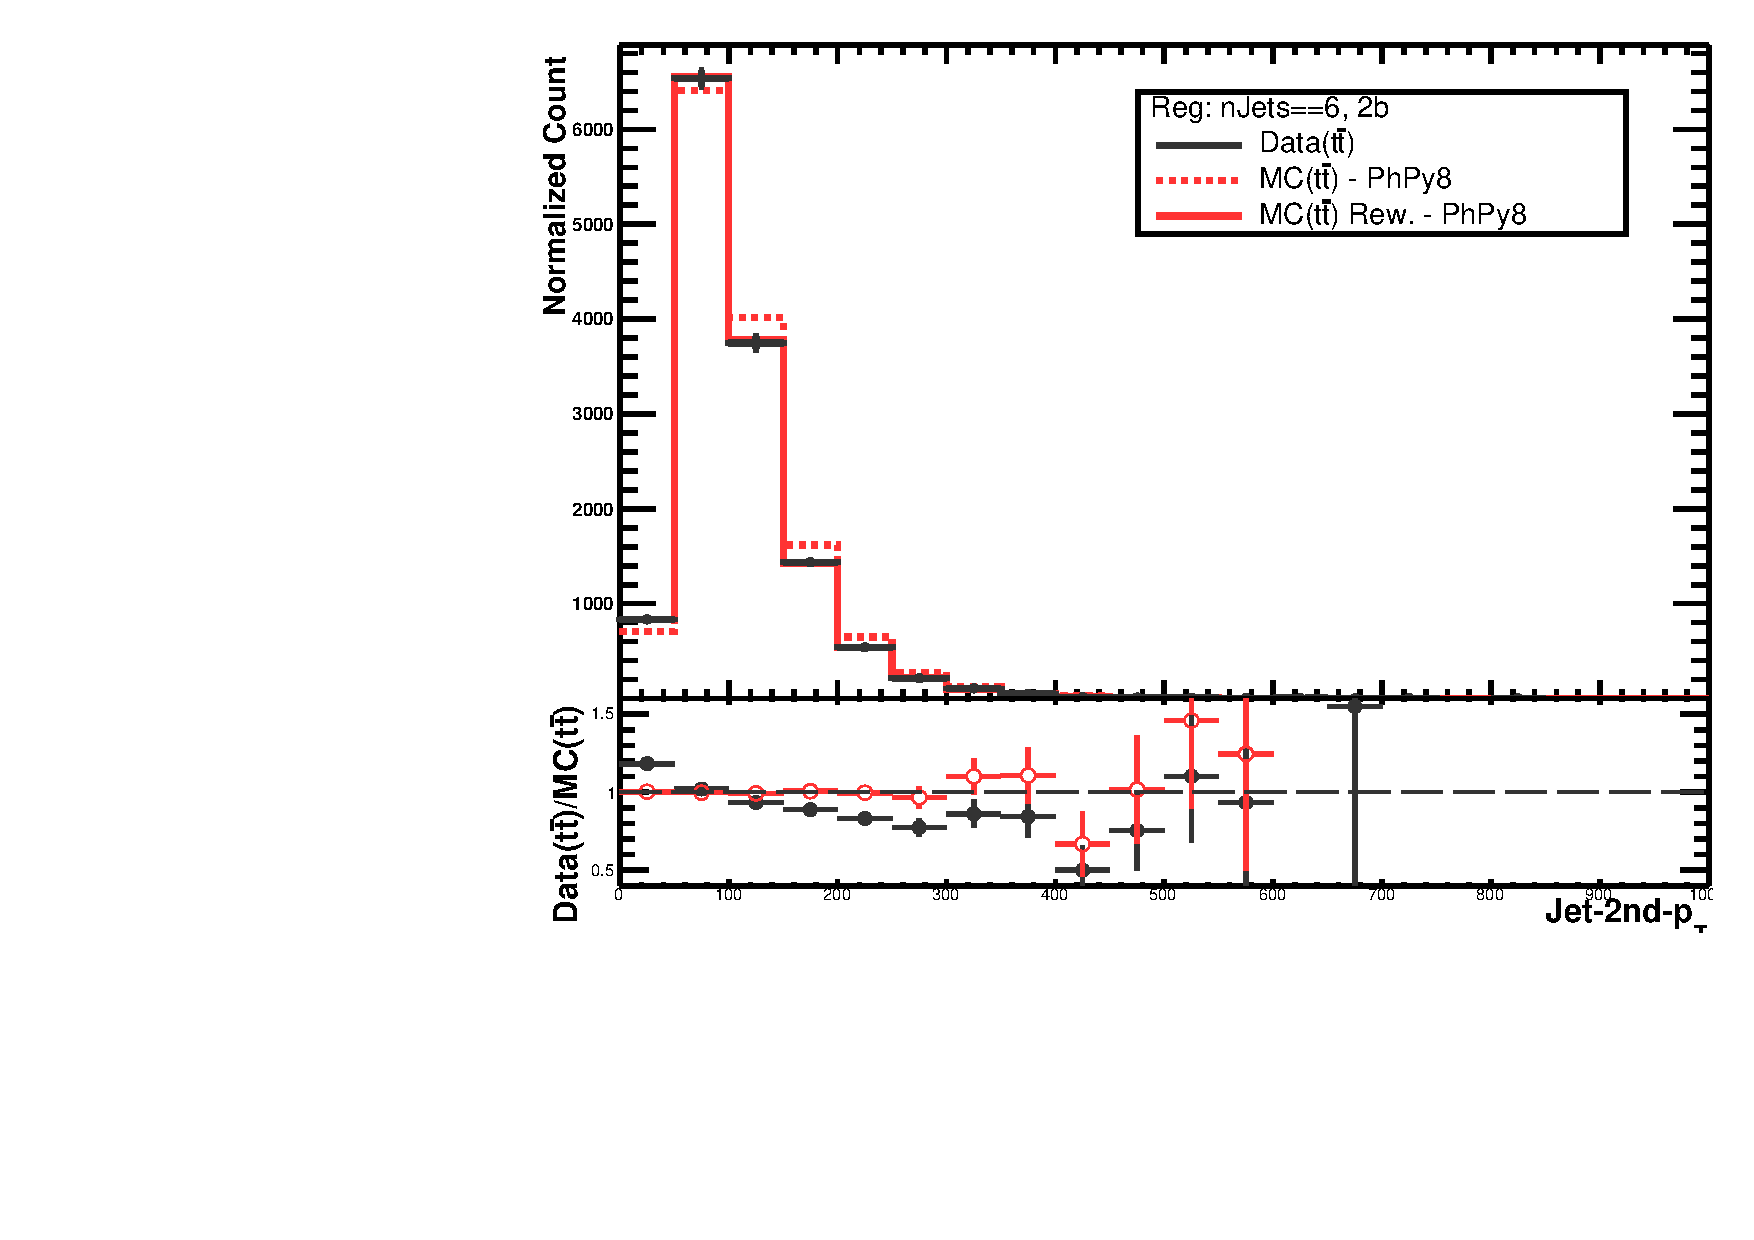
\includegraphics[width=0.24 \textwidth]{figures/rew_datamc_hfinckin_212169/1_ratiojet_pt_1__1e3_nJetsee6__2LOS.pdf} &
    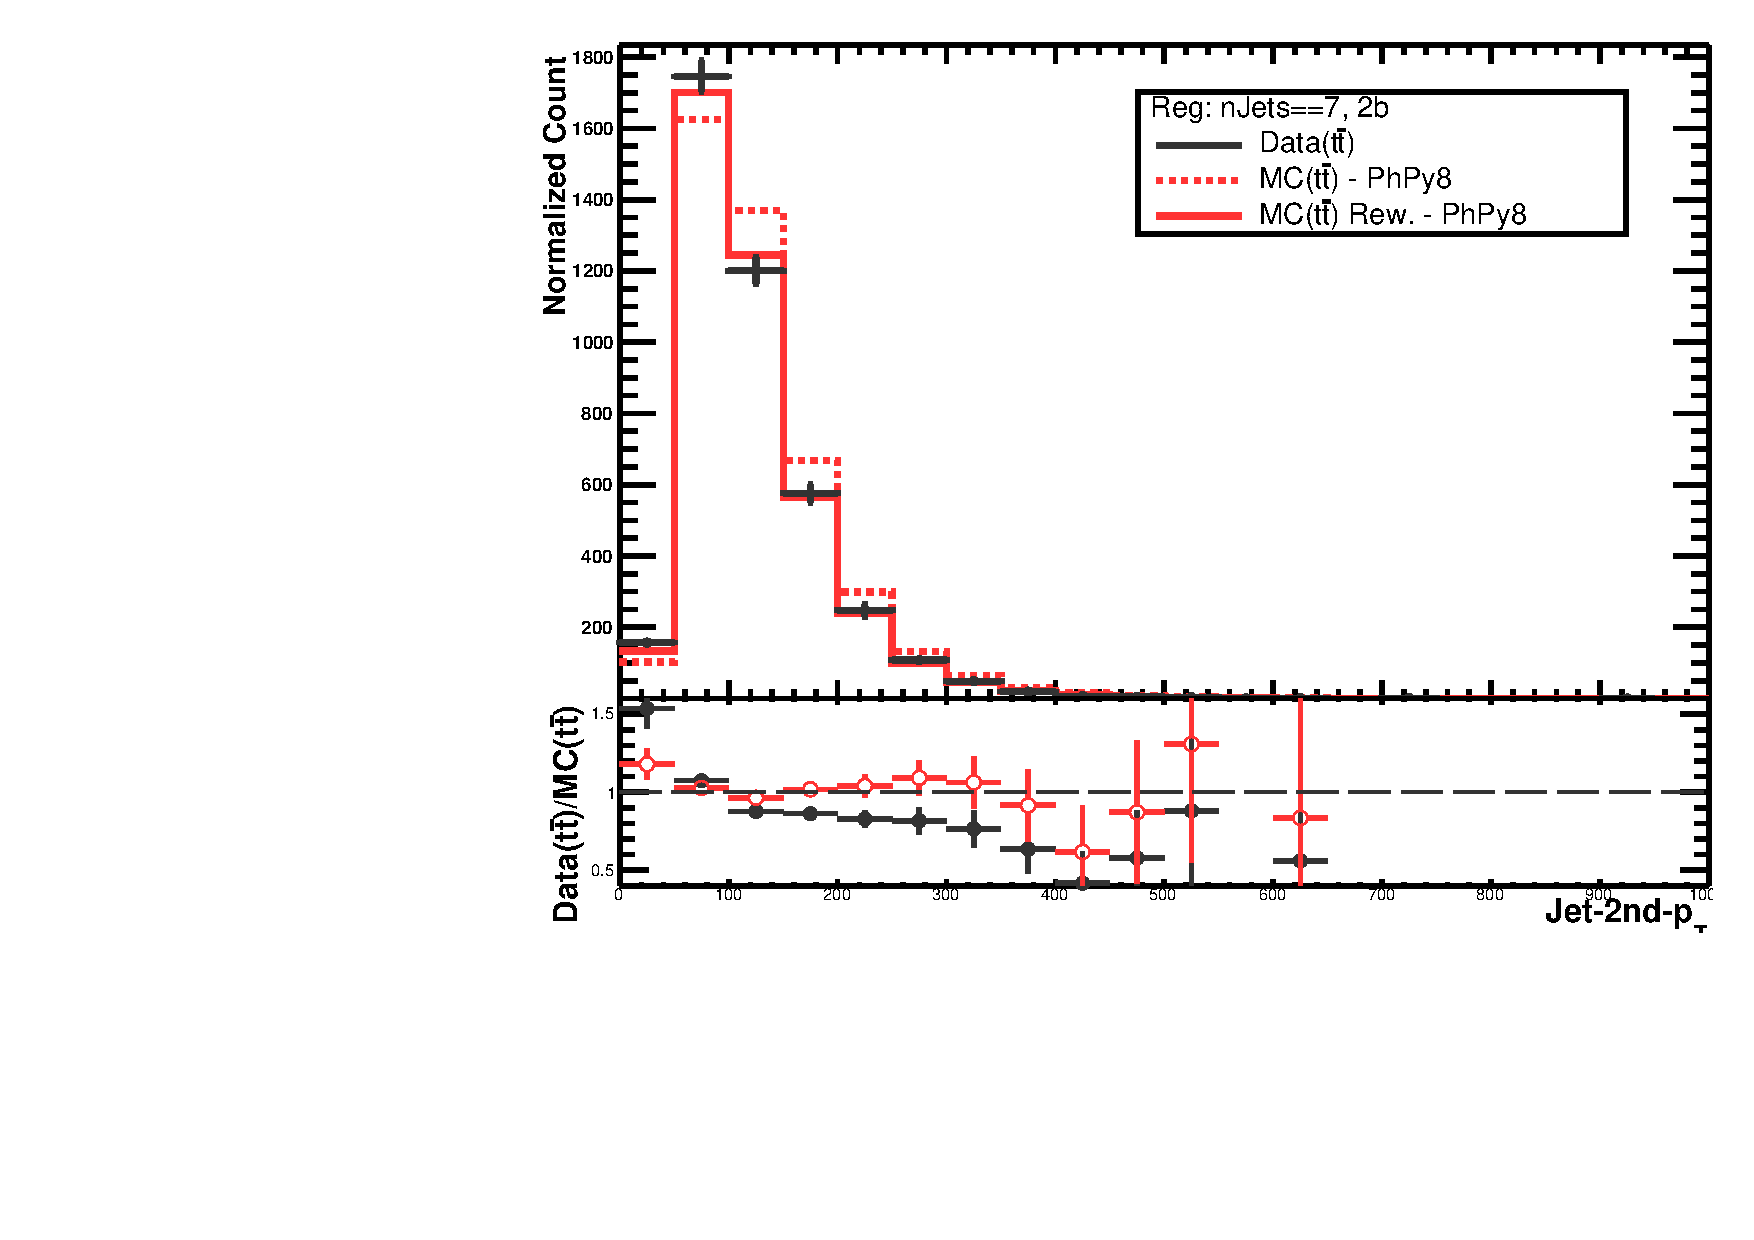
\includegraphics[width=0.24 \textwidth]{figures/rew_datamc_hfinckin_212169/1_ratiojet_pt_1__1e3_nJetsee7__2LOS.pdf} &
    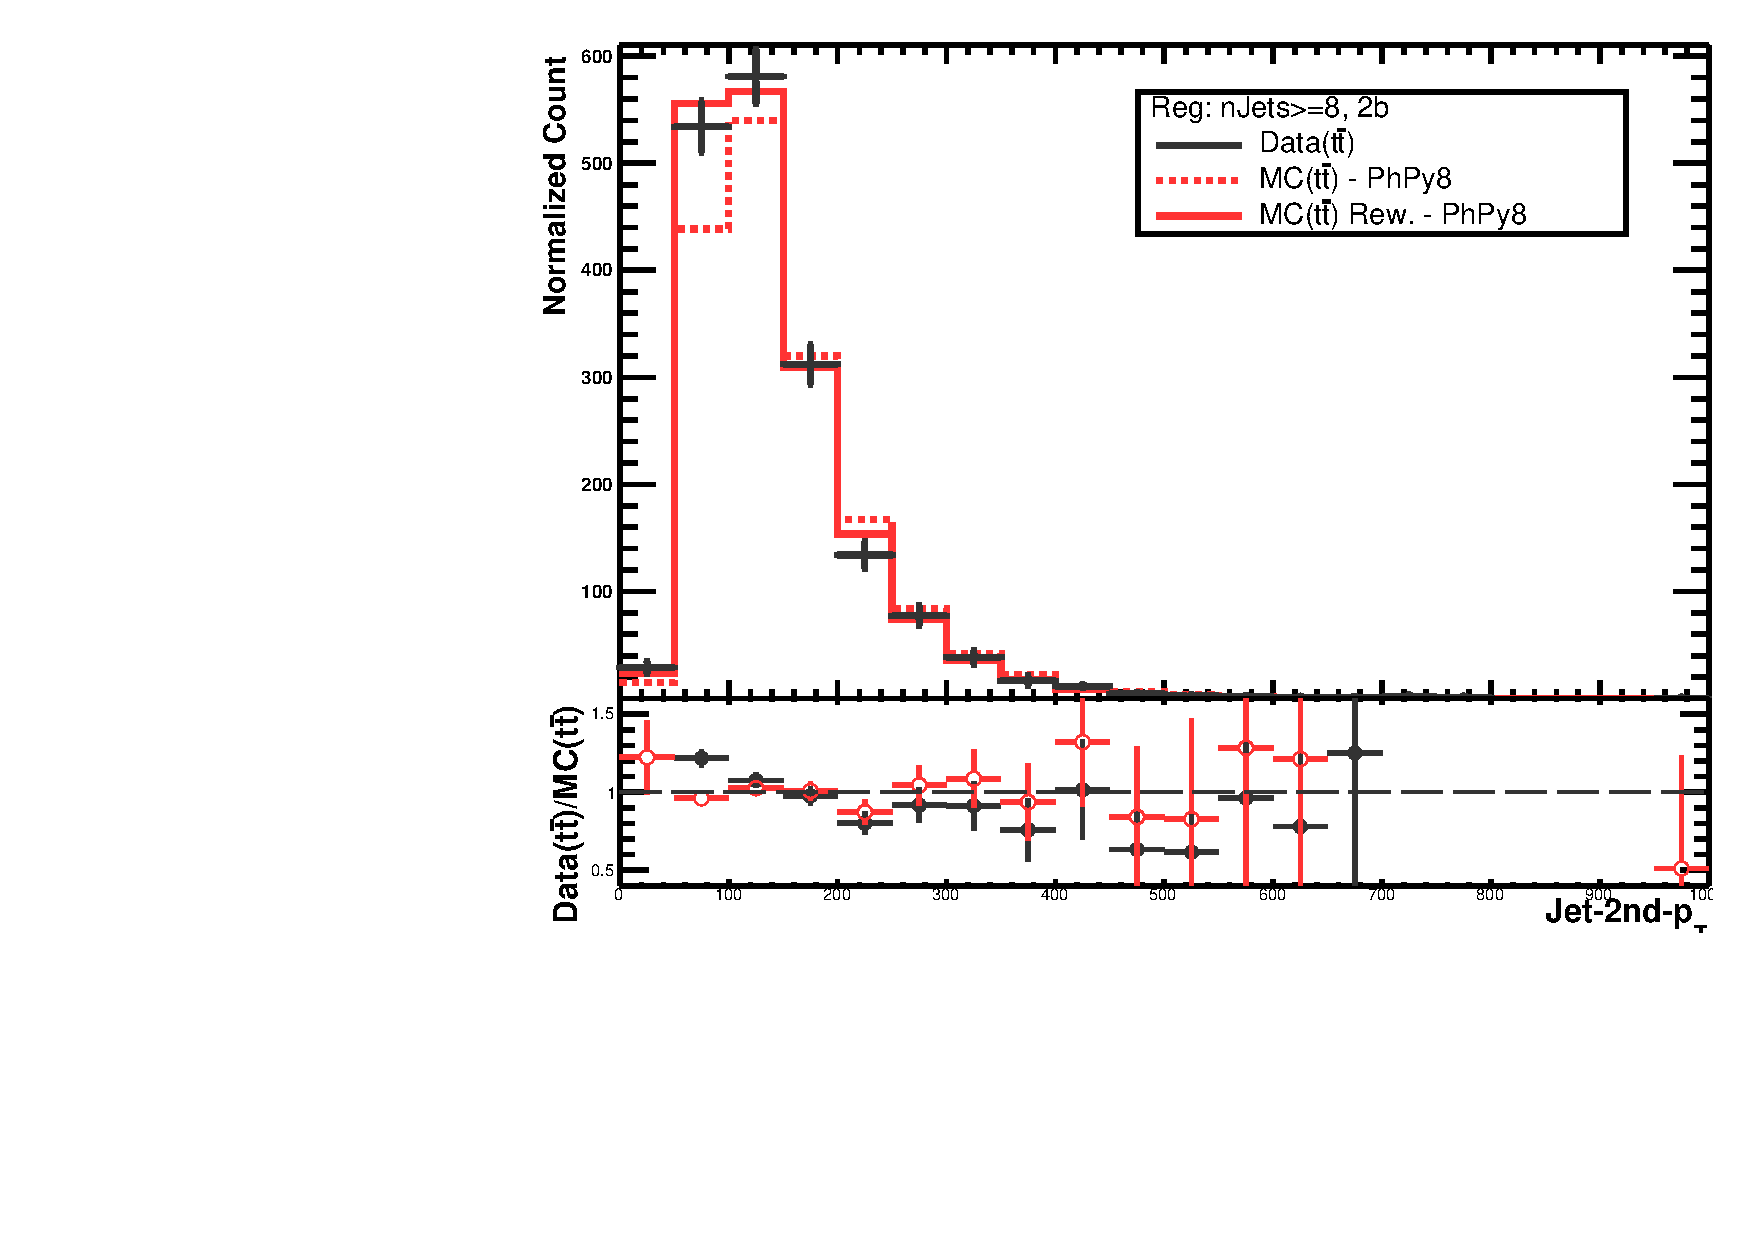
\includegraphics[width=0.24 \textwidth]{figures/rew_datamc_hfinckin_212169/1_ratiojet_pt_1__1e3_nJetsge8__2LOS.pdf} \\

    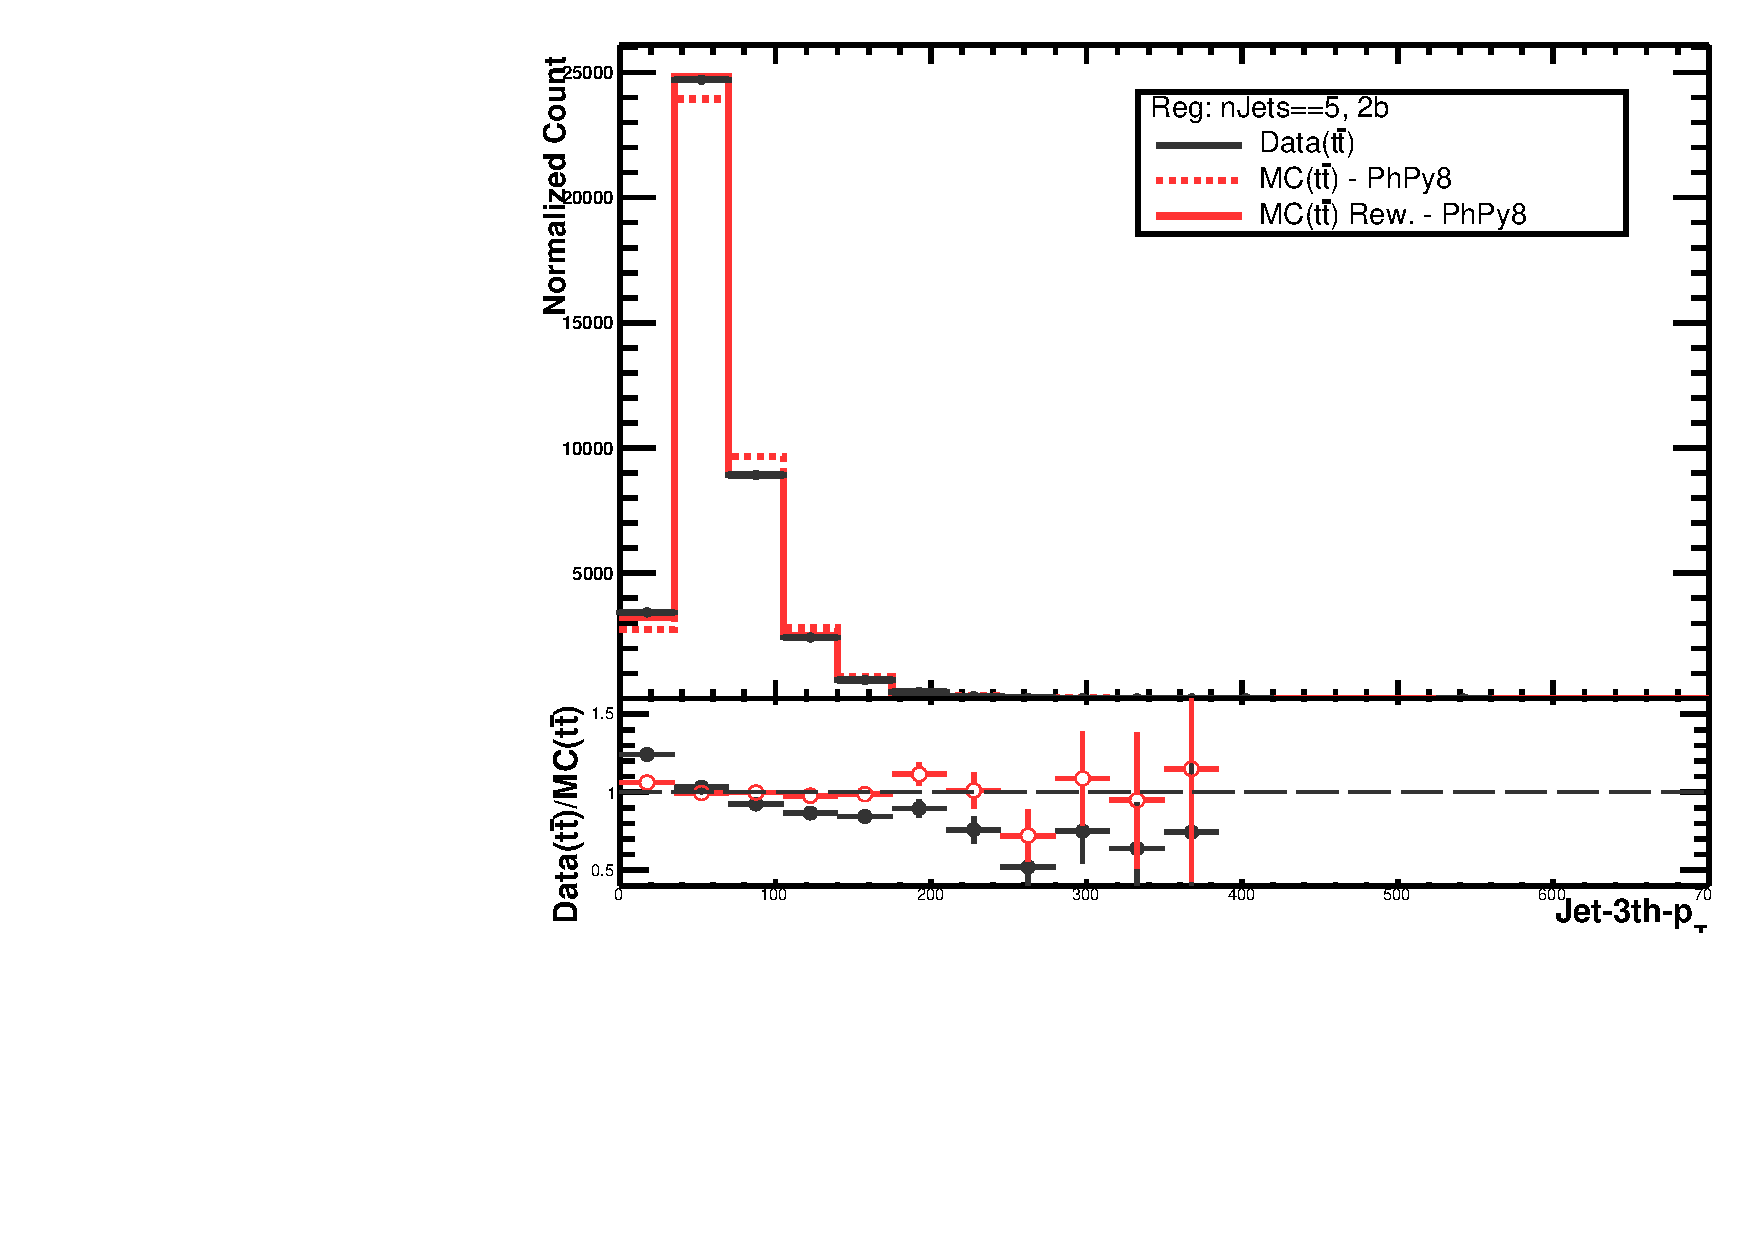
\includegraphics[width=0.24 \textwidth]{figures/rew_datamc_hfinckin_212169/1_ratiojet_pt_2__1e3_nJetsee5__2LOS.pdf} &
    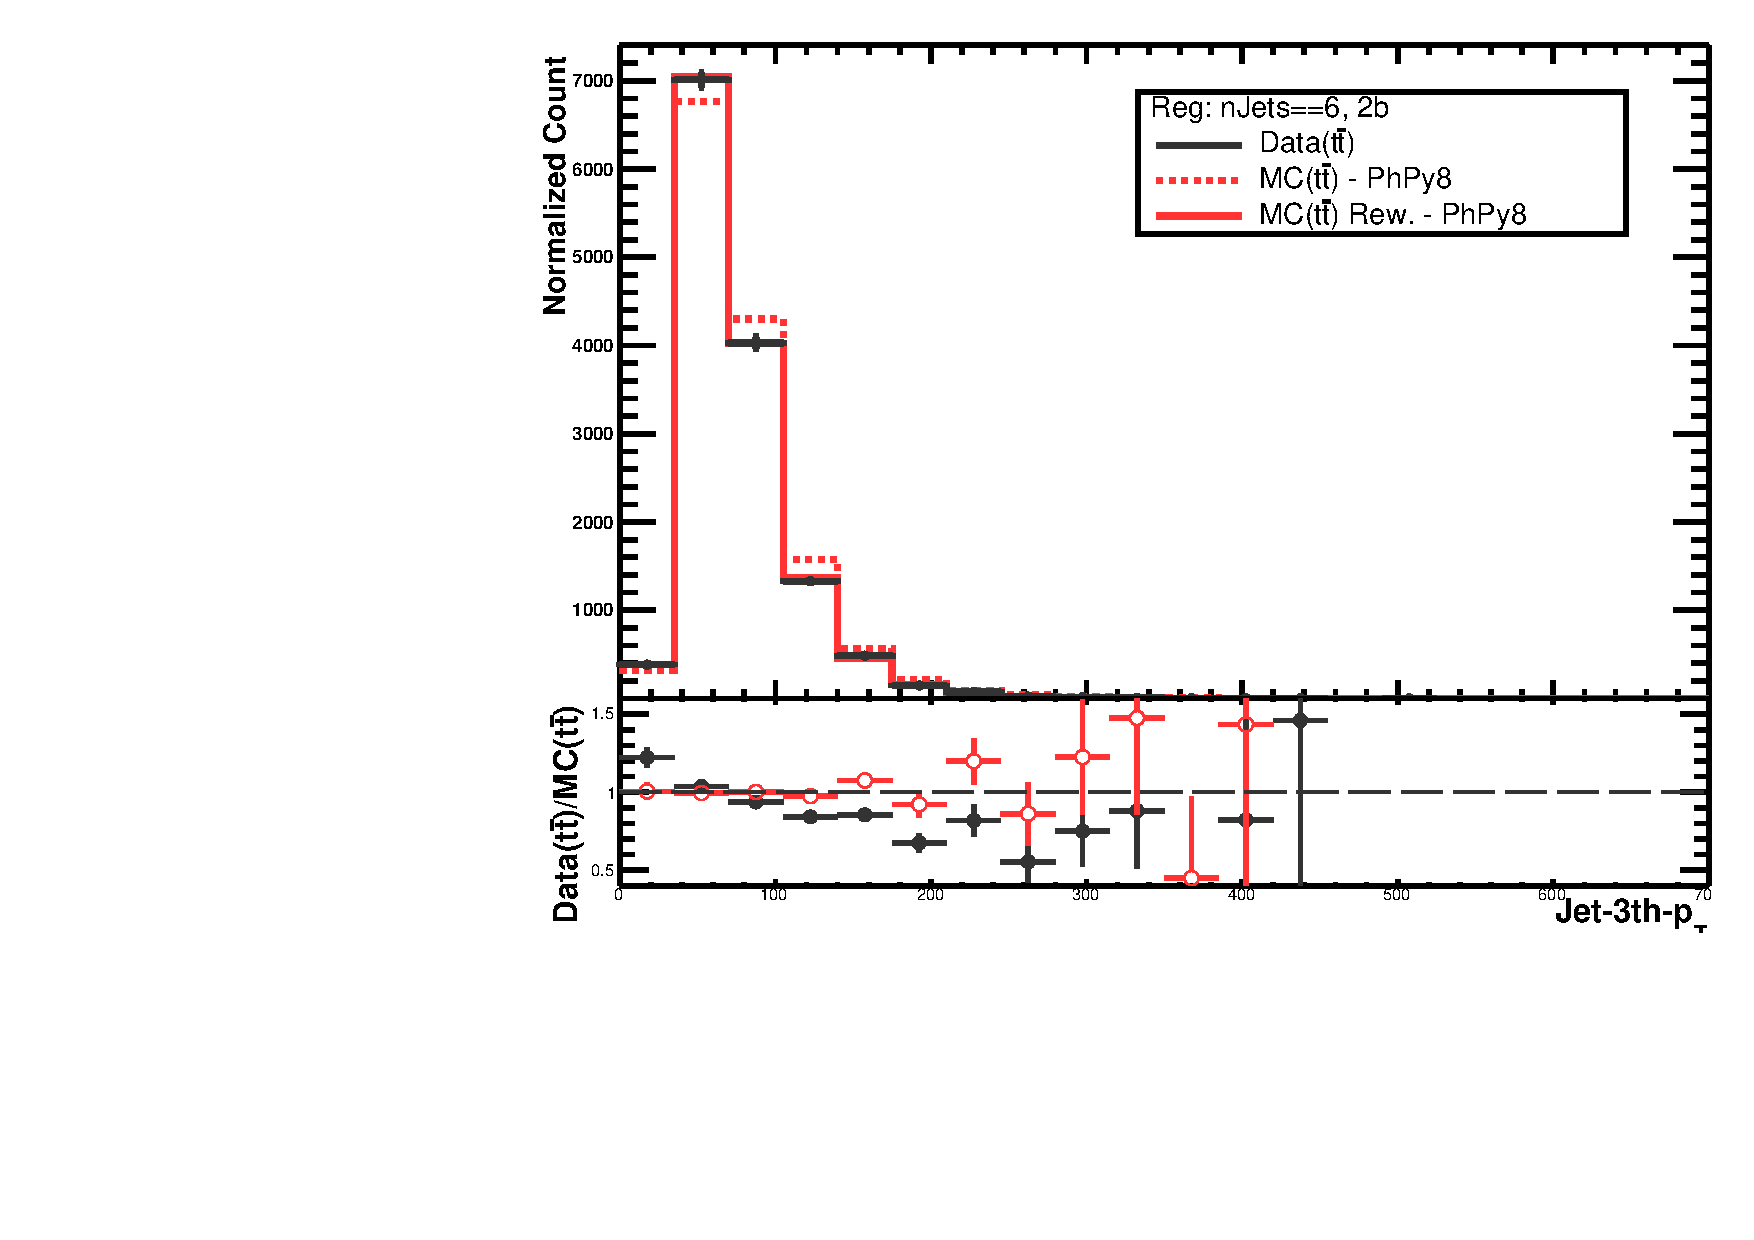
\includegraphics[width=0.24 \textwidth]{figures/rew_datamc_hfinckin_212169/1_ratiojet_pt_2__1e3_nJetsee6__2LOS.pdf} &
    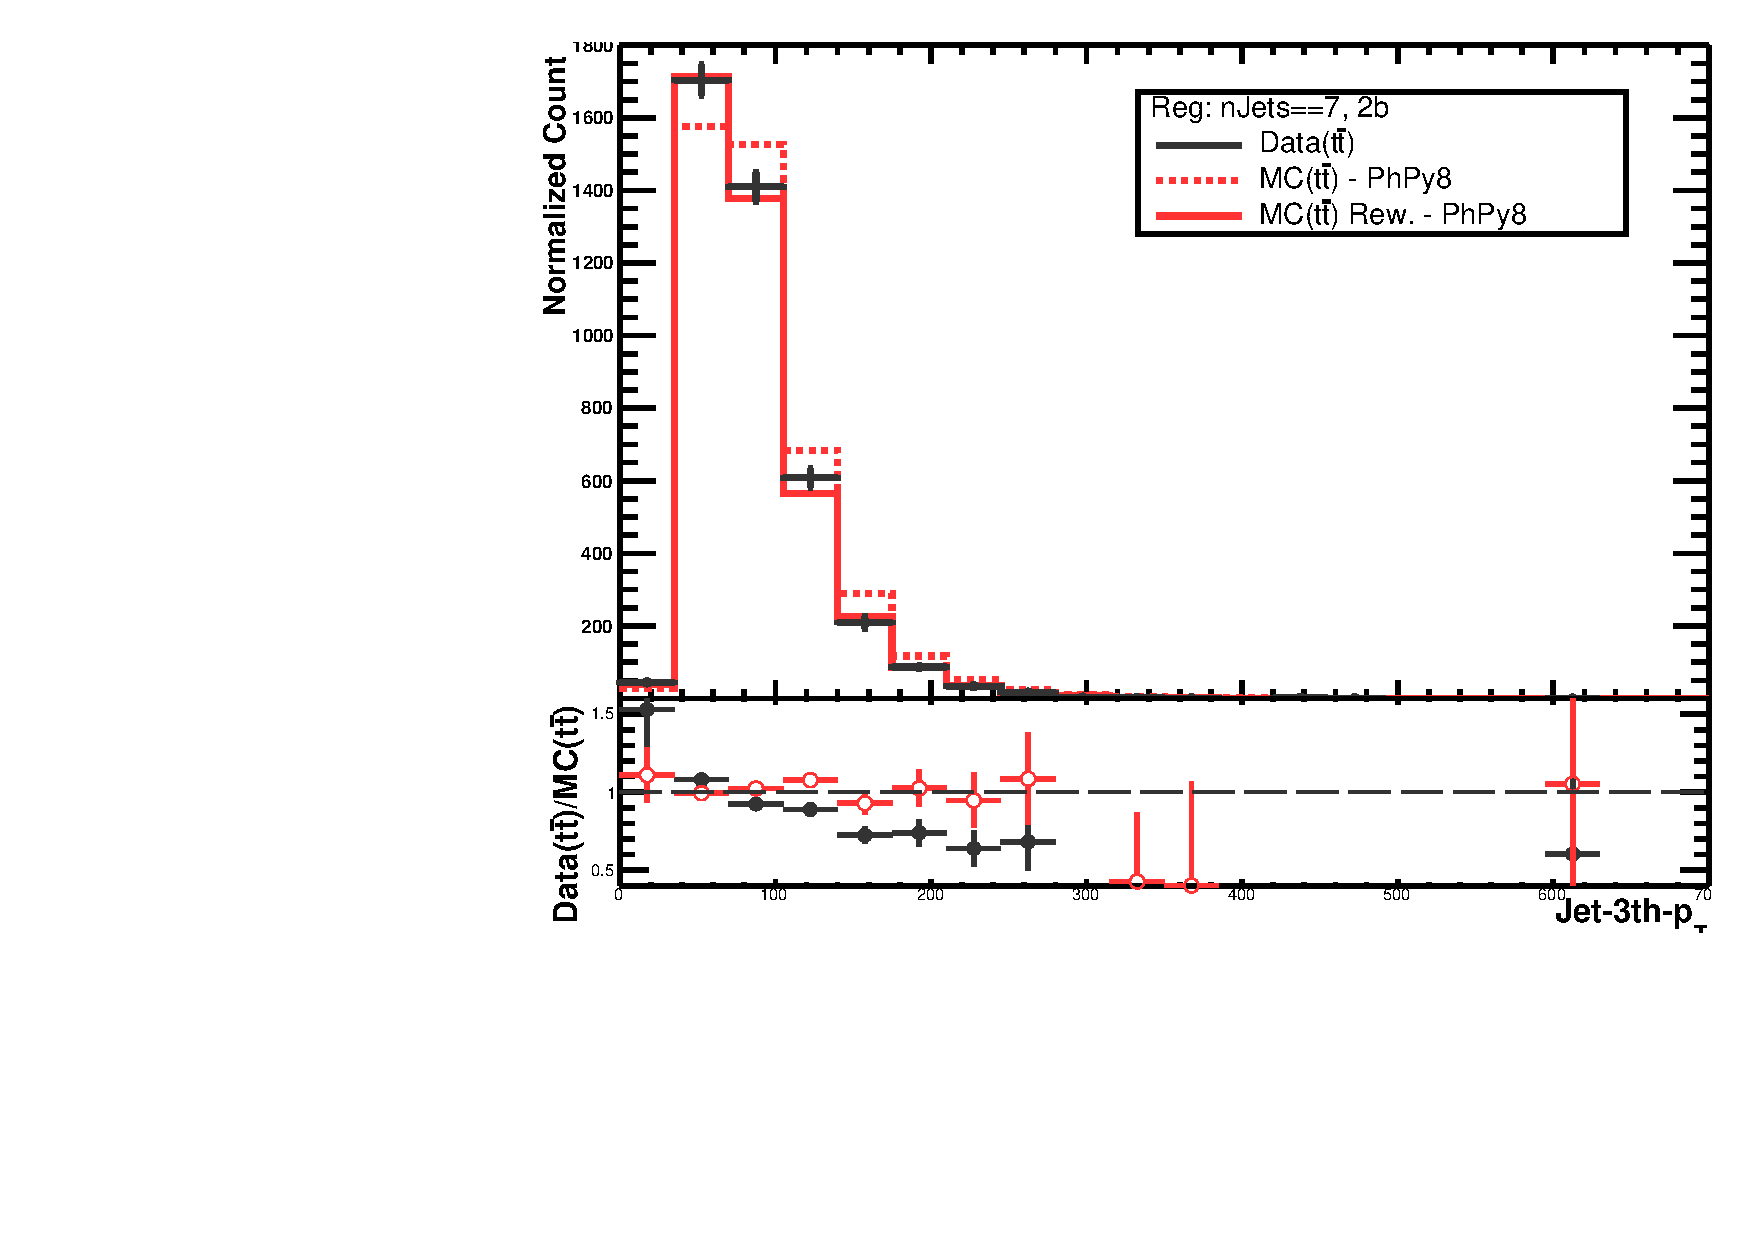
\includegraphics[width=0.24 \textwidth]{figures/rew_datamc_hfinckin_212169/1_ratiojet_pt_2__1e3_nJetsee7__2LOS.pdf} &
    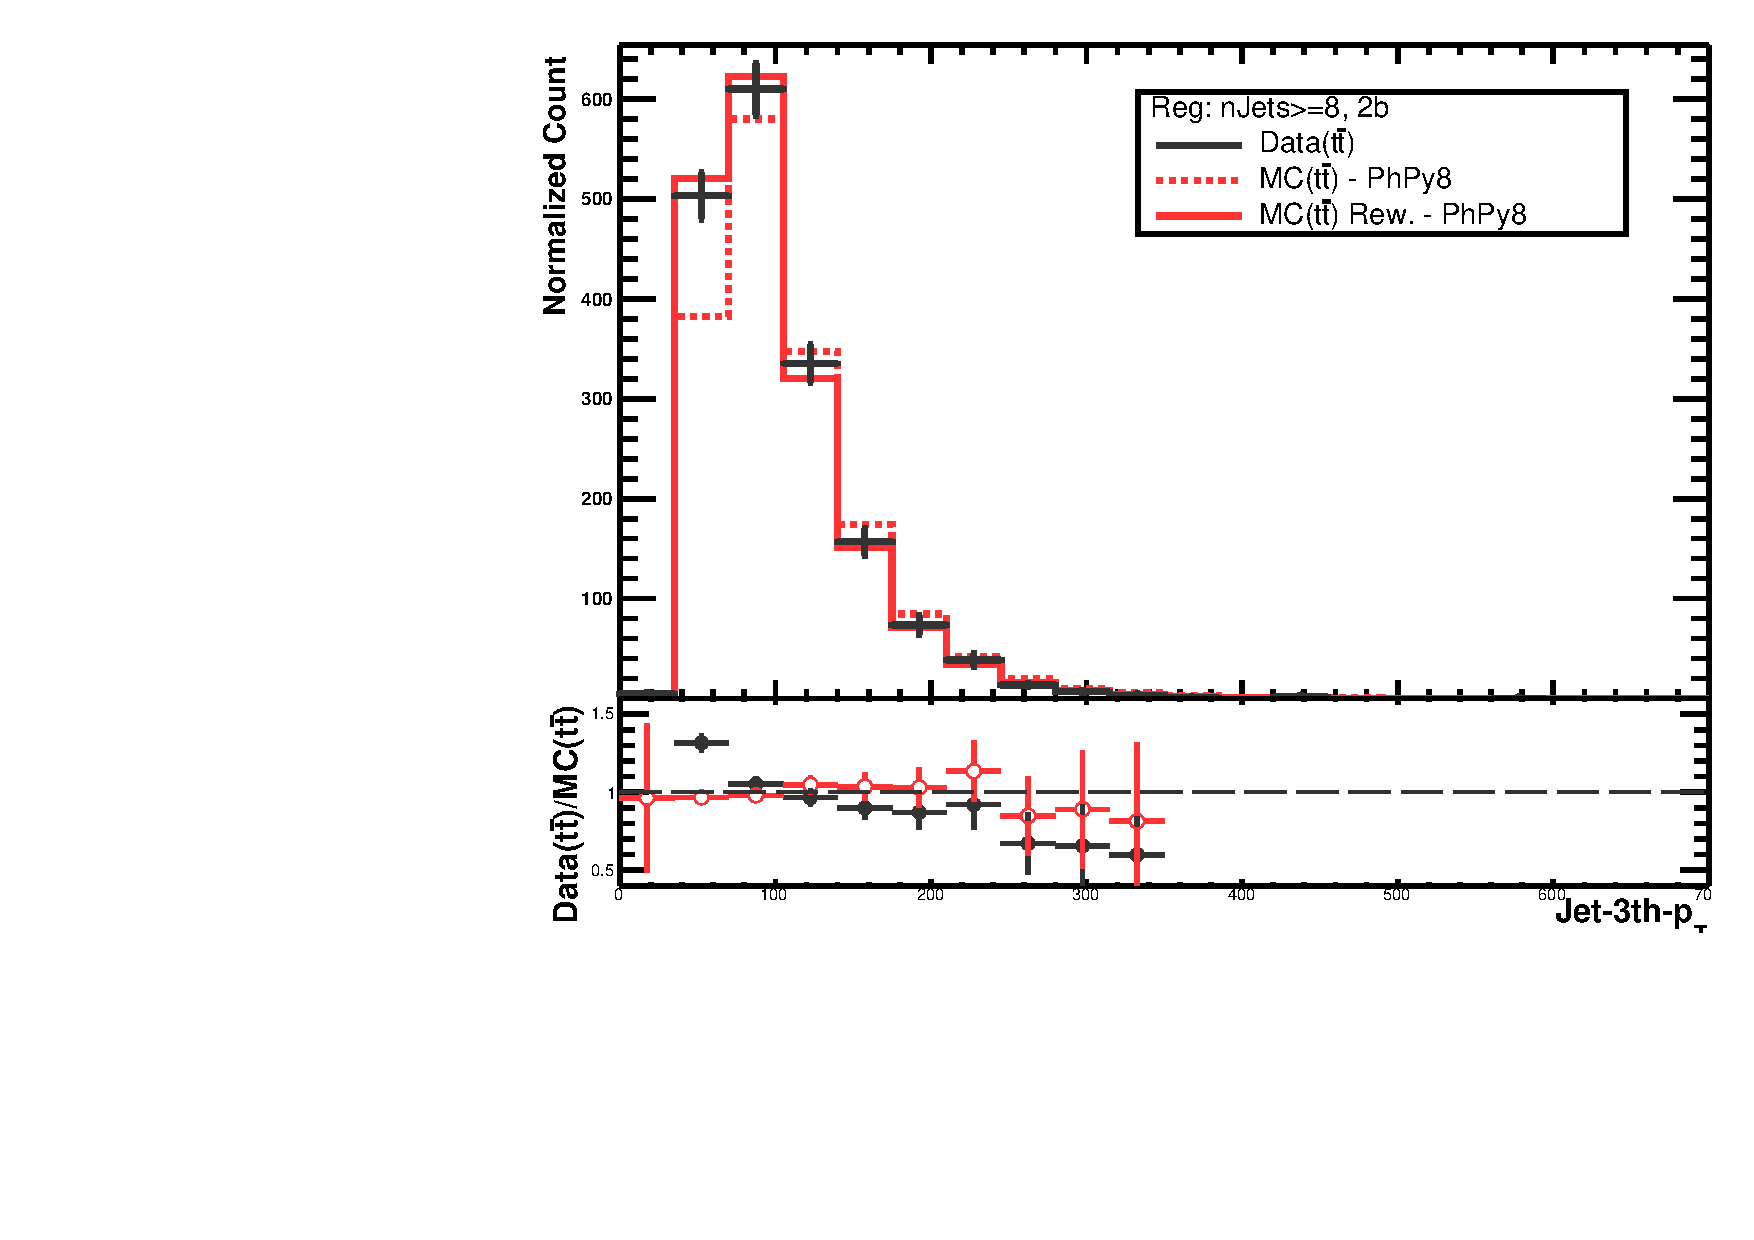
\includegraphics[width=0.24 \textwidth]{figures/rew_datamc_hfinckin_212169/1_ratiojet_pt_2__1e3_nJetsge8__2LOS.pdf} \\

    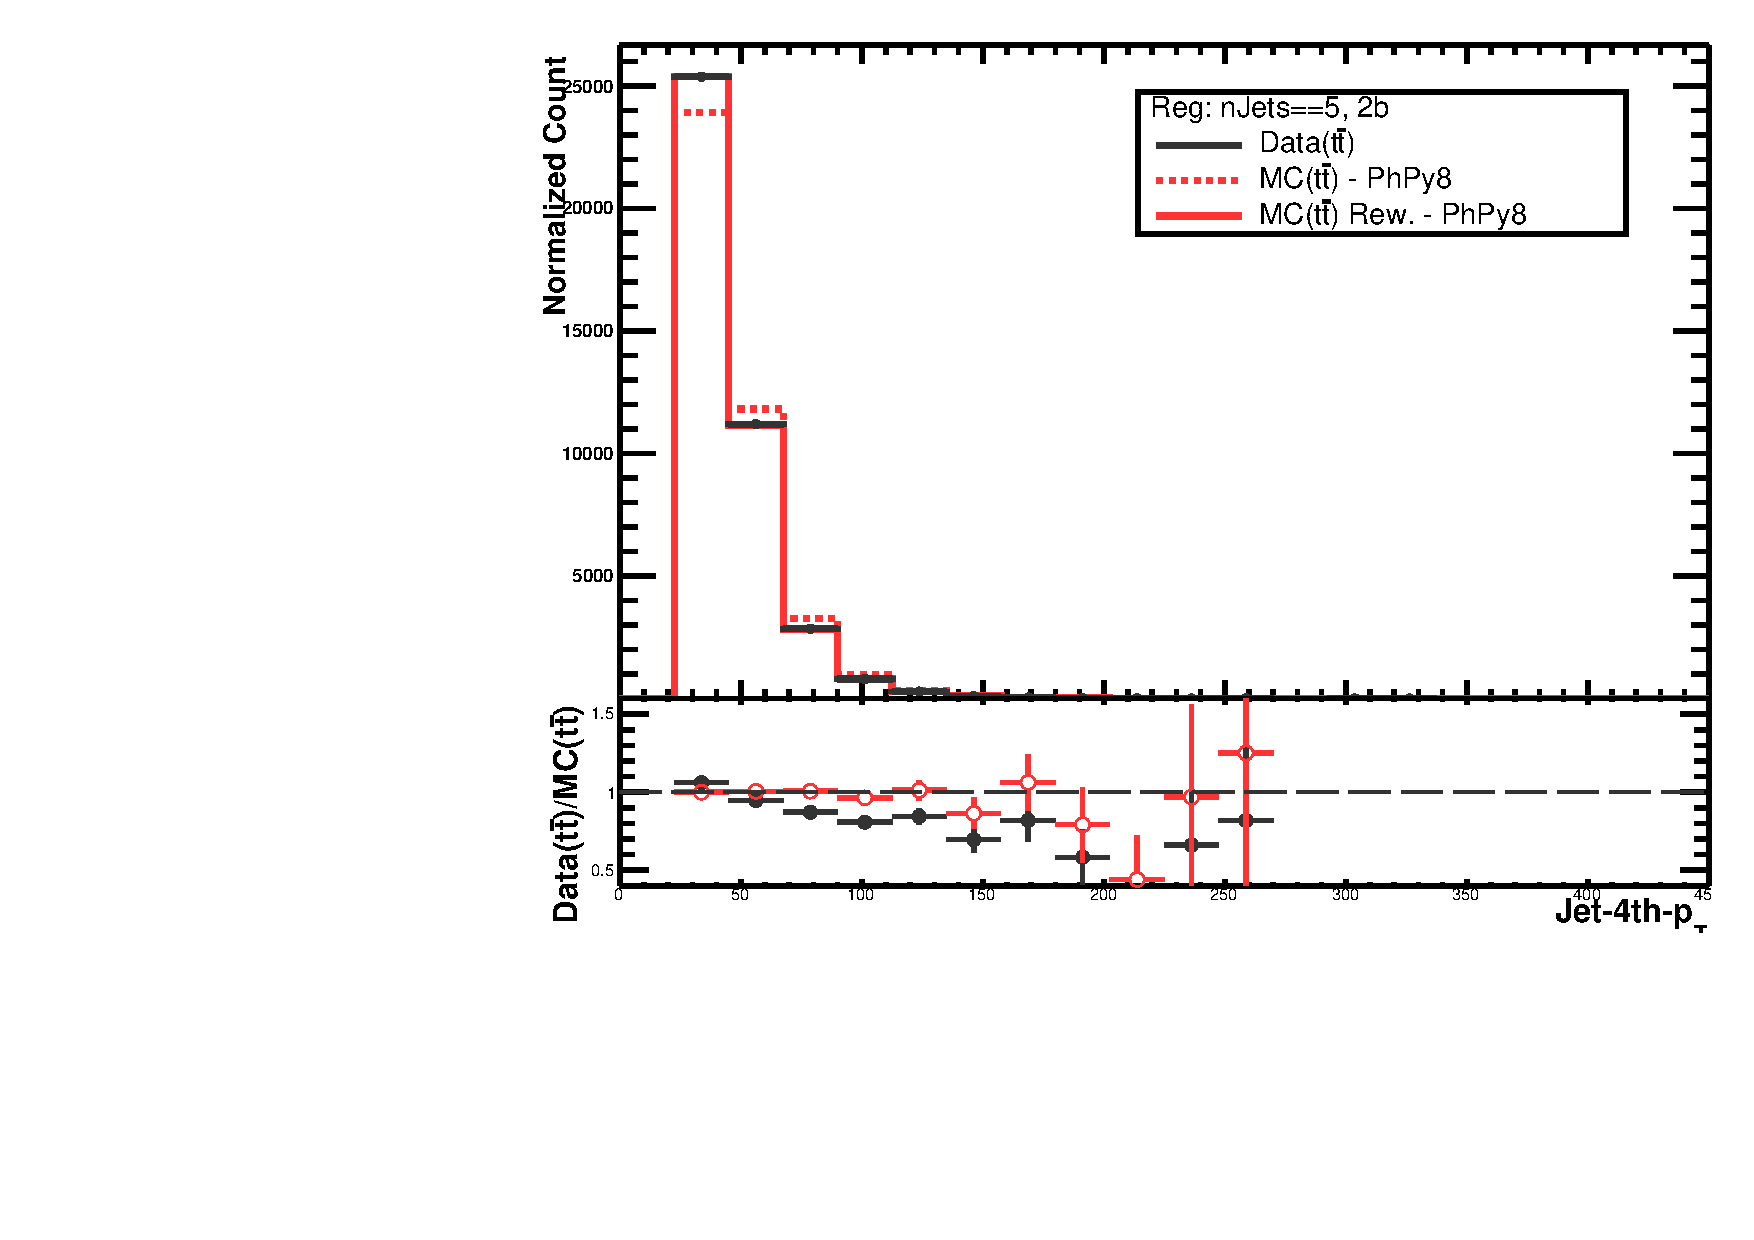
\includegraphics[width=0.24 \textwidth]{figures/rew_datamc_hfinckin_212169/1_ratiojet_pt_3__1e3_nJetsee5__2LOS.pdf} &
    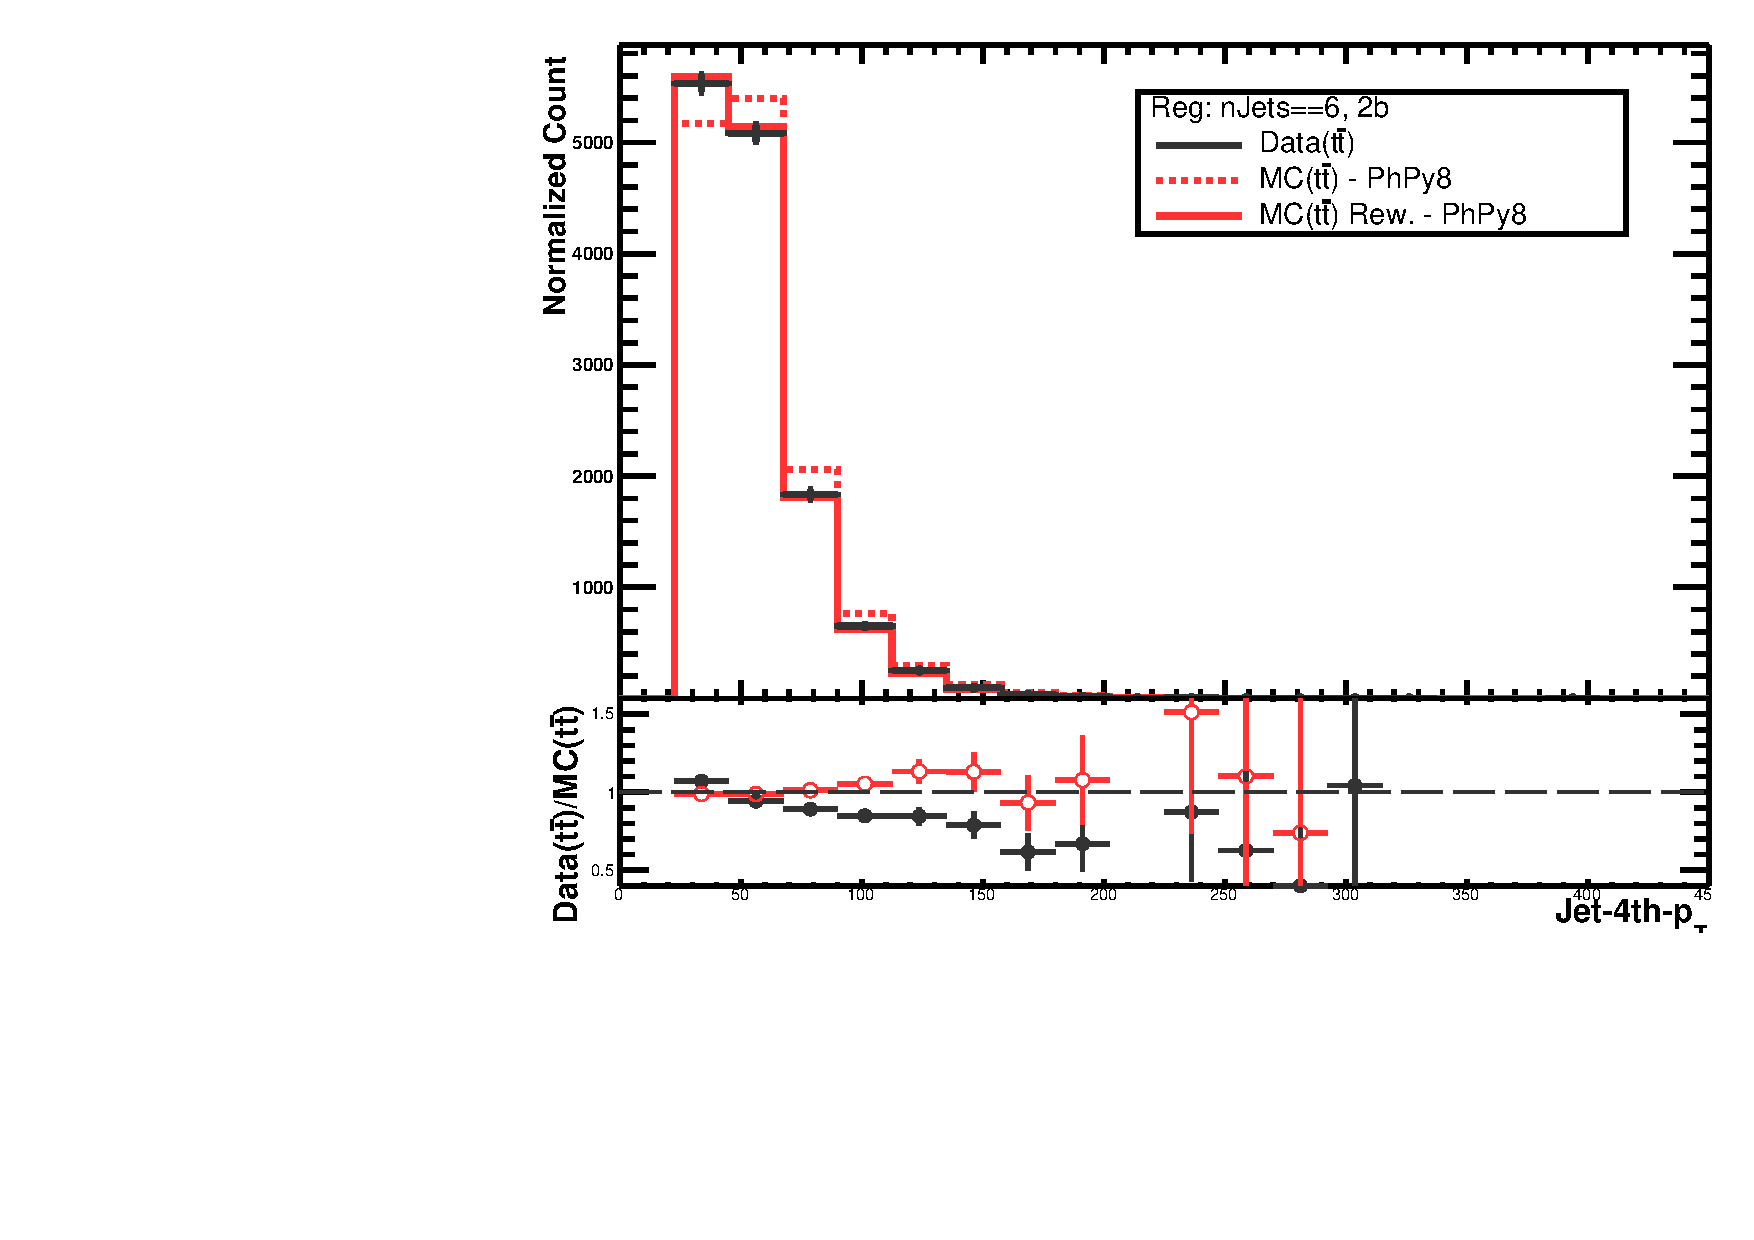
\includegraphics[width=0.24 \textwidth]{figures/rew_datamc_hfinckin_212169/1_ratiojet_pt_3__1e3_nJetsee6__2LOS.pdf} &
    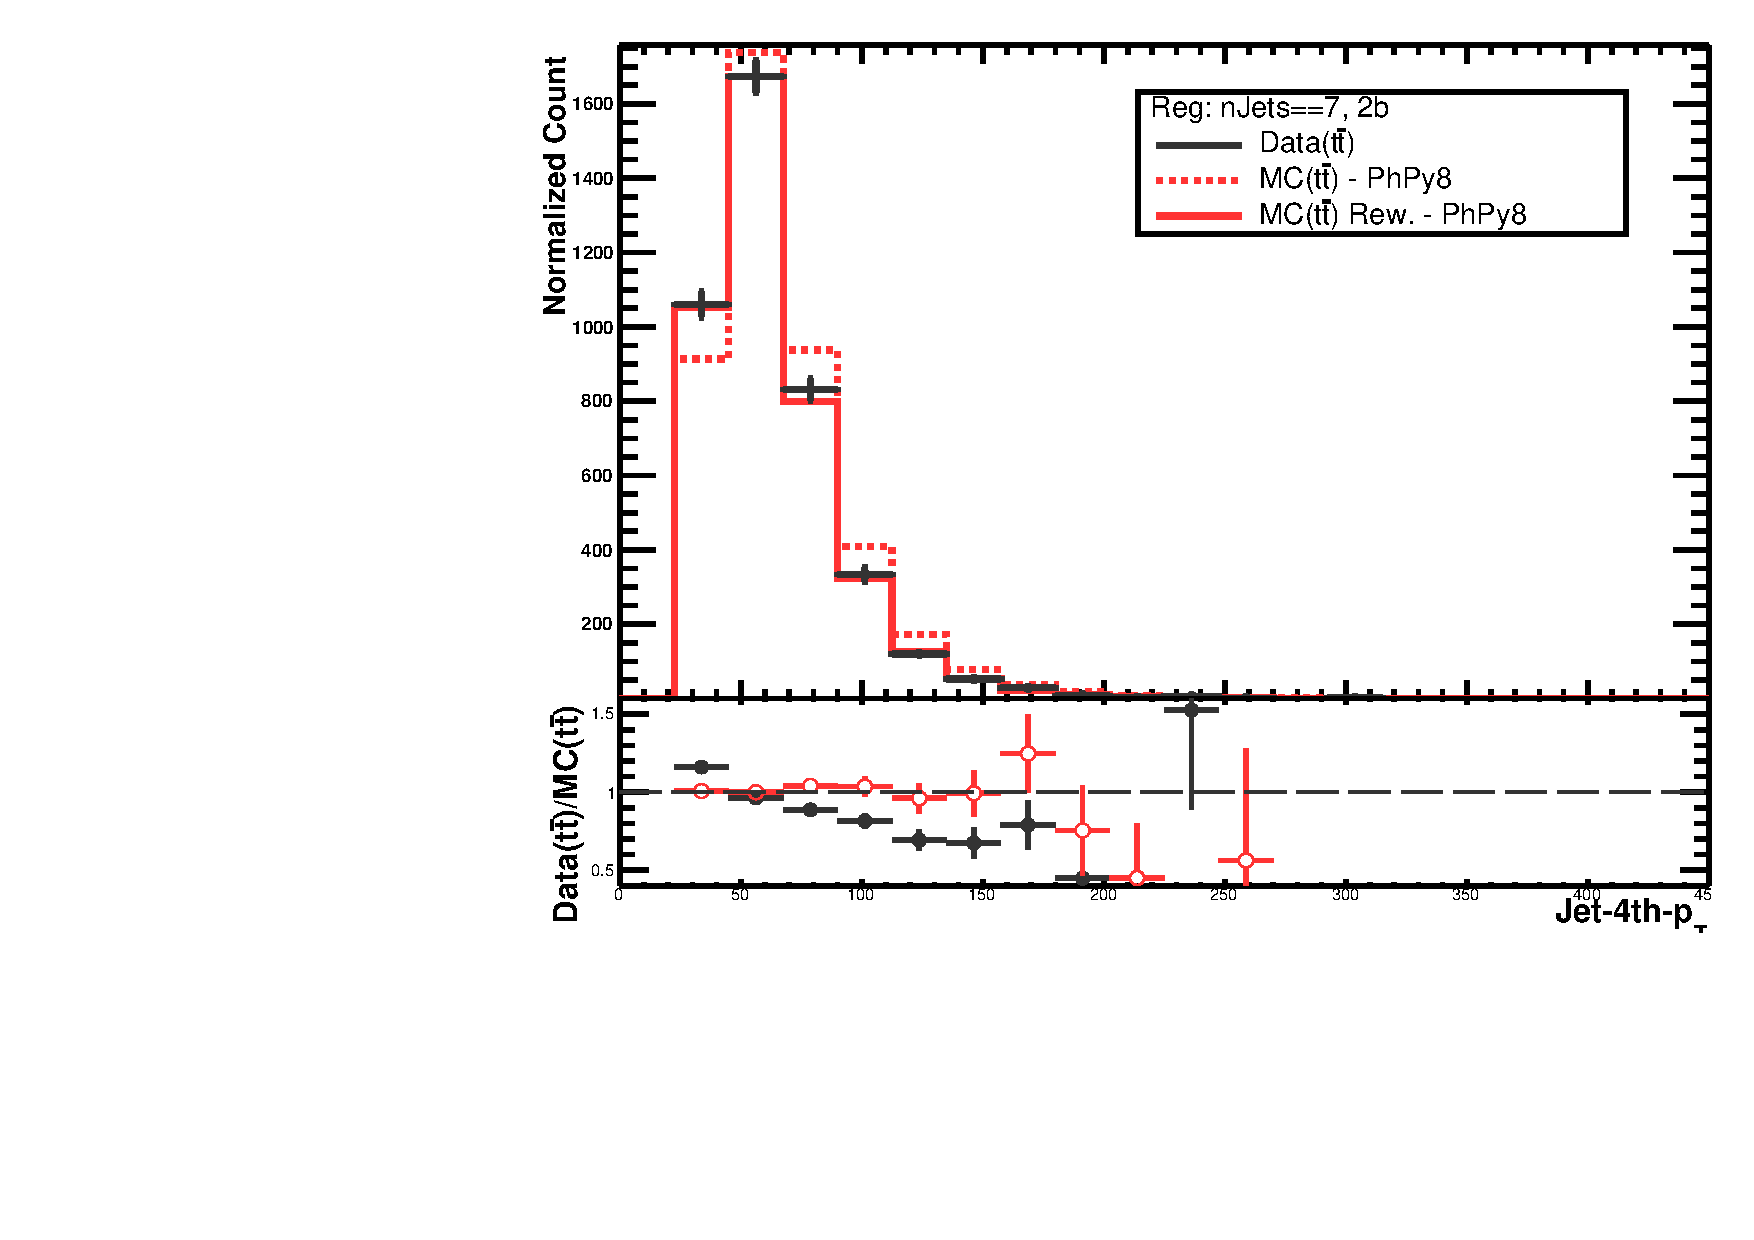
\includegraphics[width=0.24 \textwidth]{figures/rew_datamc_hfinckin_212169/1_ratiojet_pt_3__1e3_nJetsee7__2LOS.pdf} &
    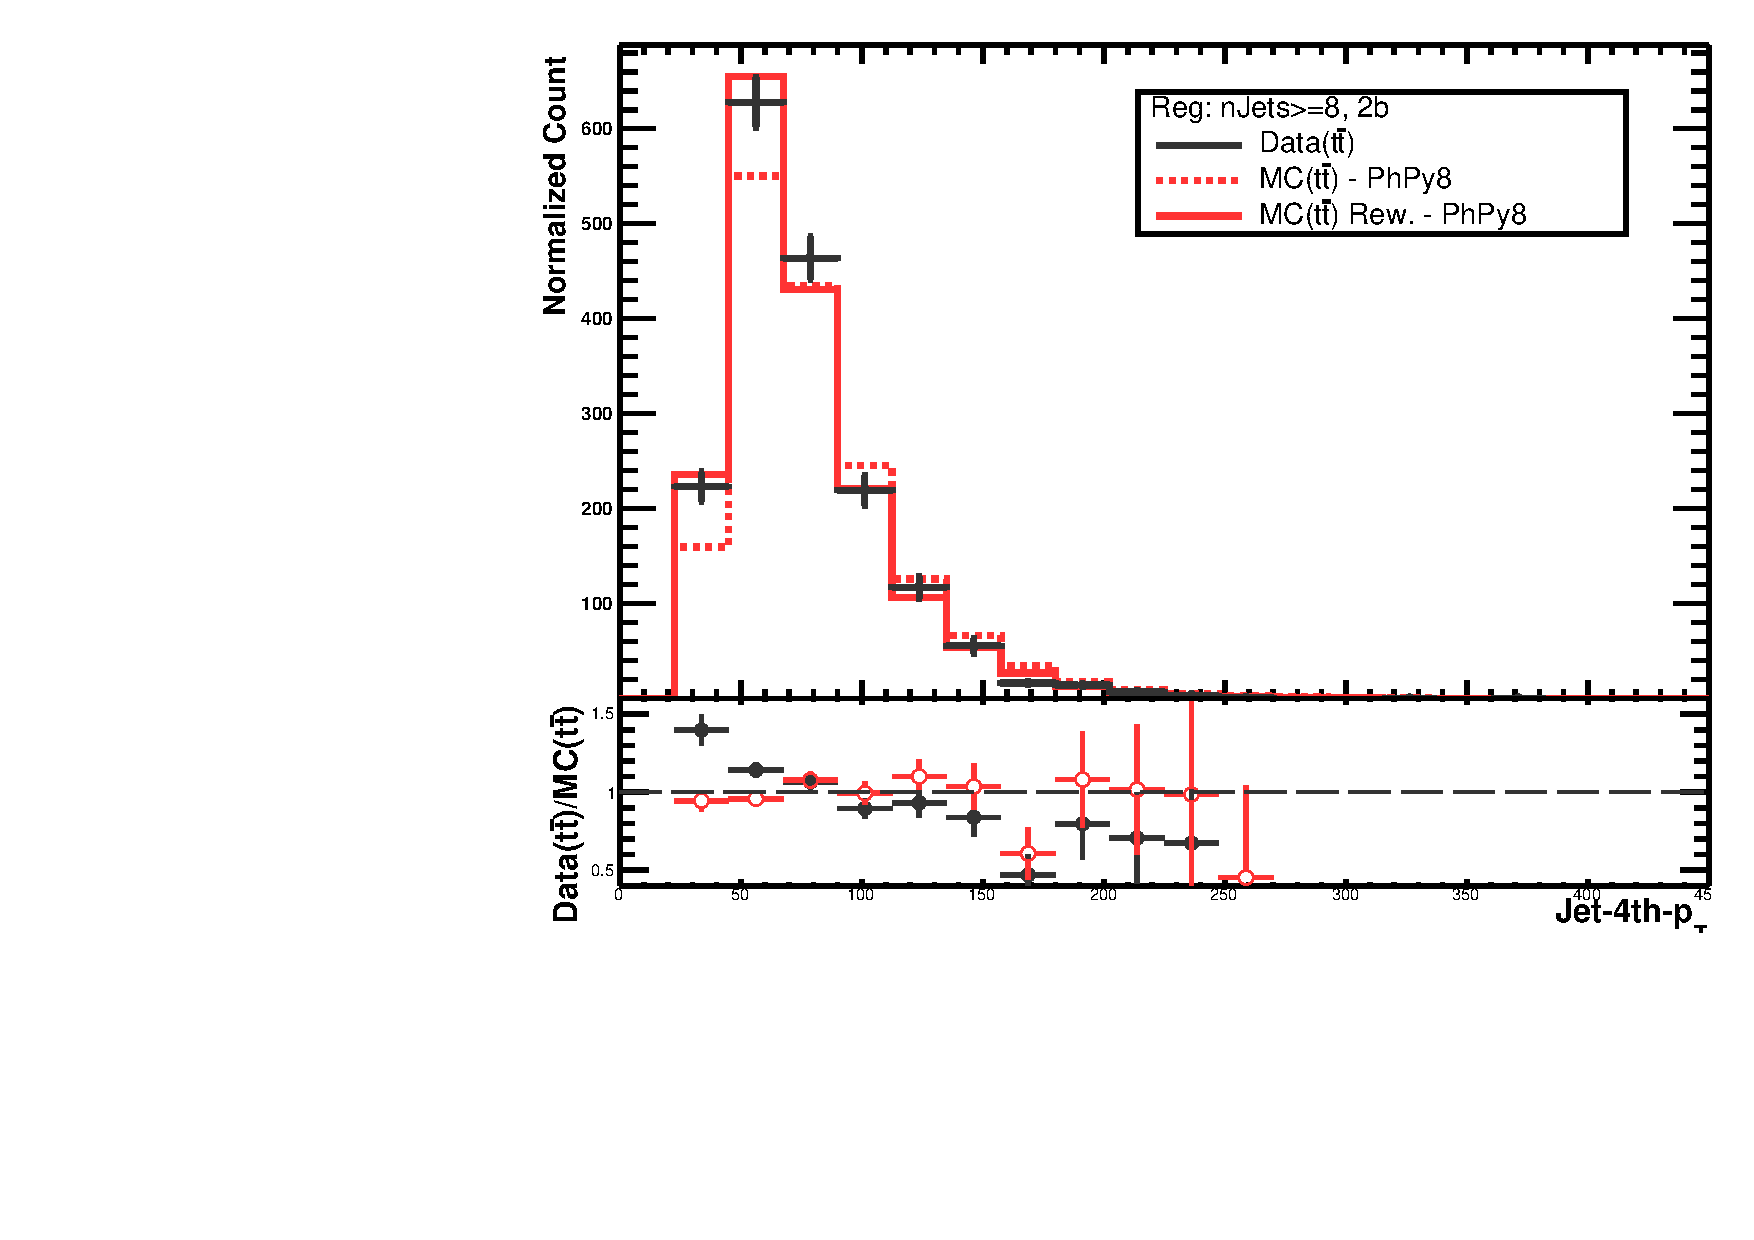
\includegraphics[width=0.24 \textwidth]{figures/rew_datamc_hfinckin_212169/1_ratiojet_pt_3__1e3_nJetsge8__2LOS.pdf} \\

    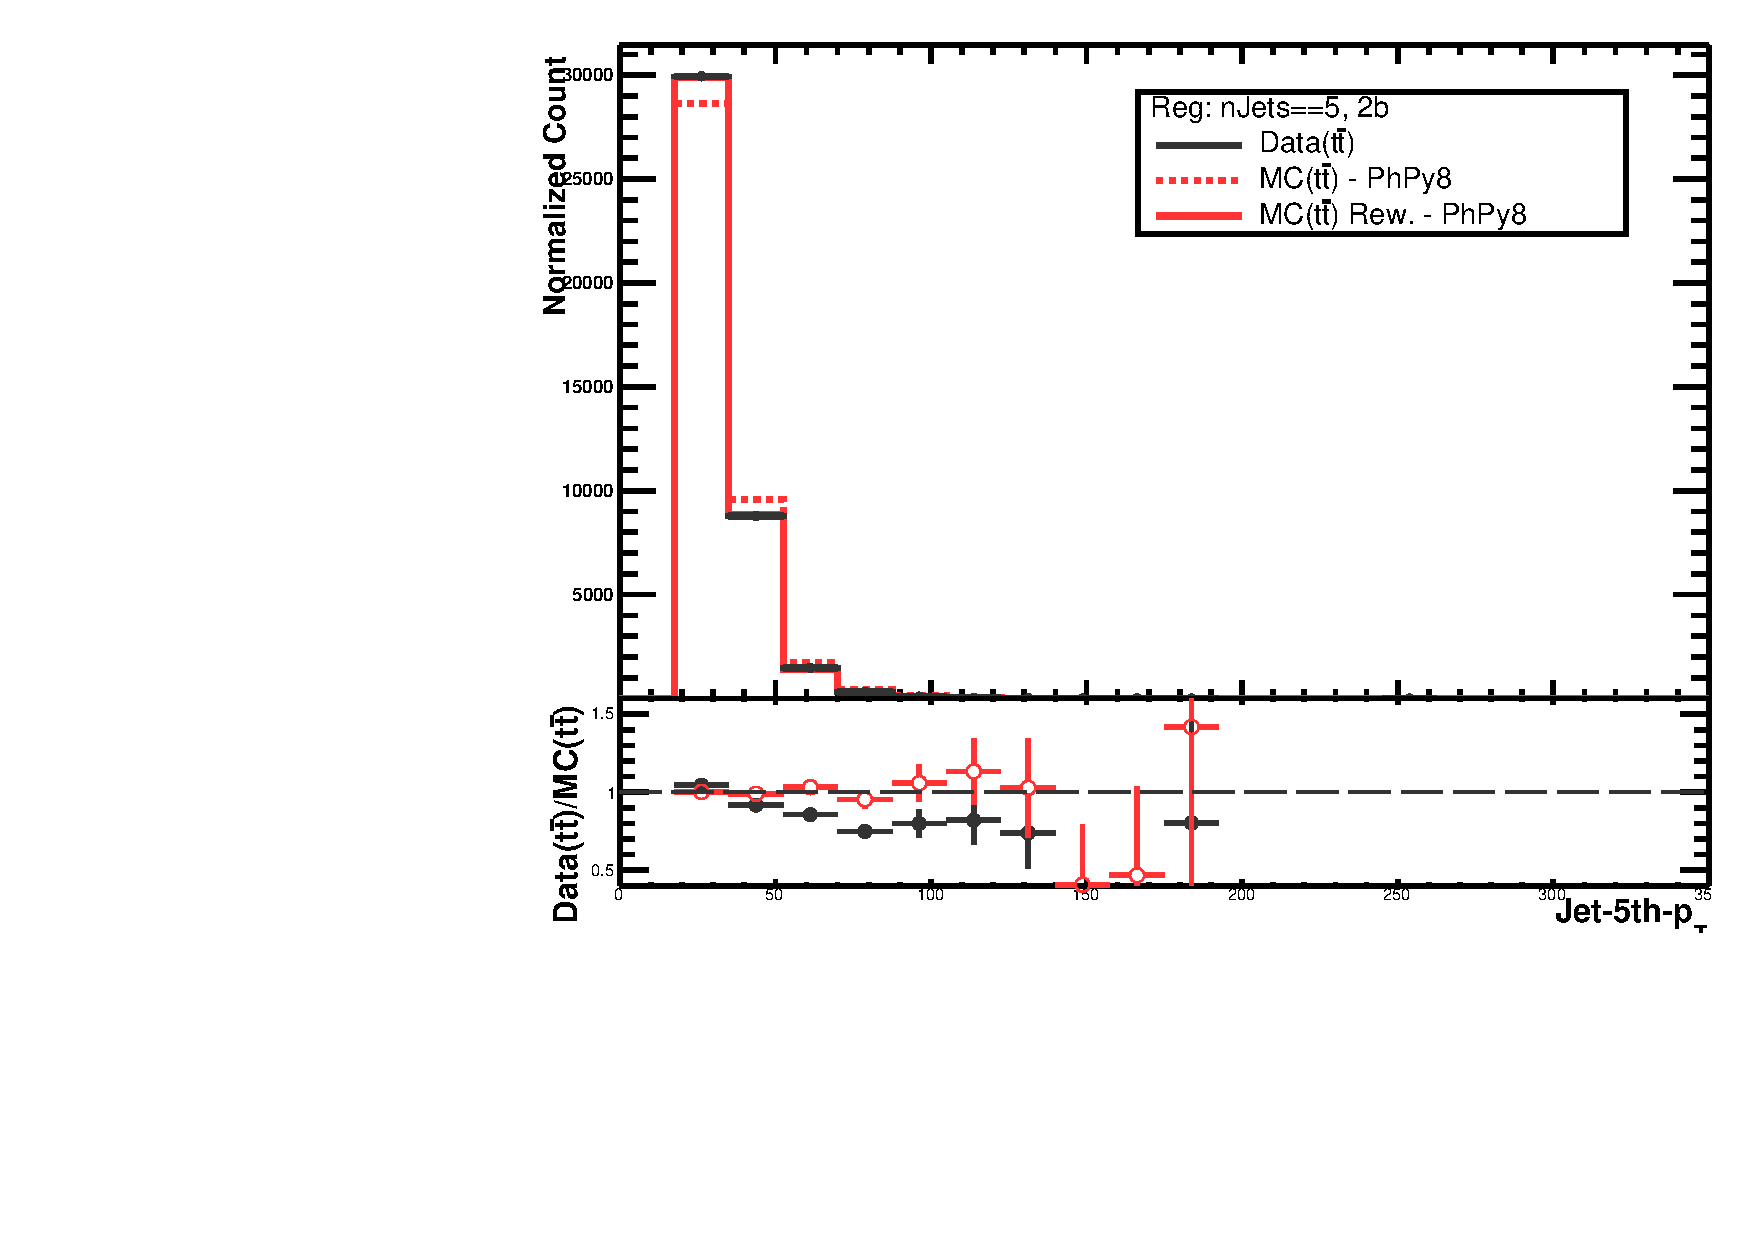
\includegraphics[width=0.24 \textwidth]{figures/rew_datamc_hfinckin_212169/1_ratiojet_pt_4__1e3_nJetsee5__2LOS.pdf} &
    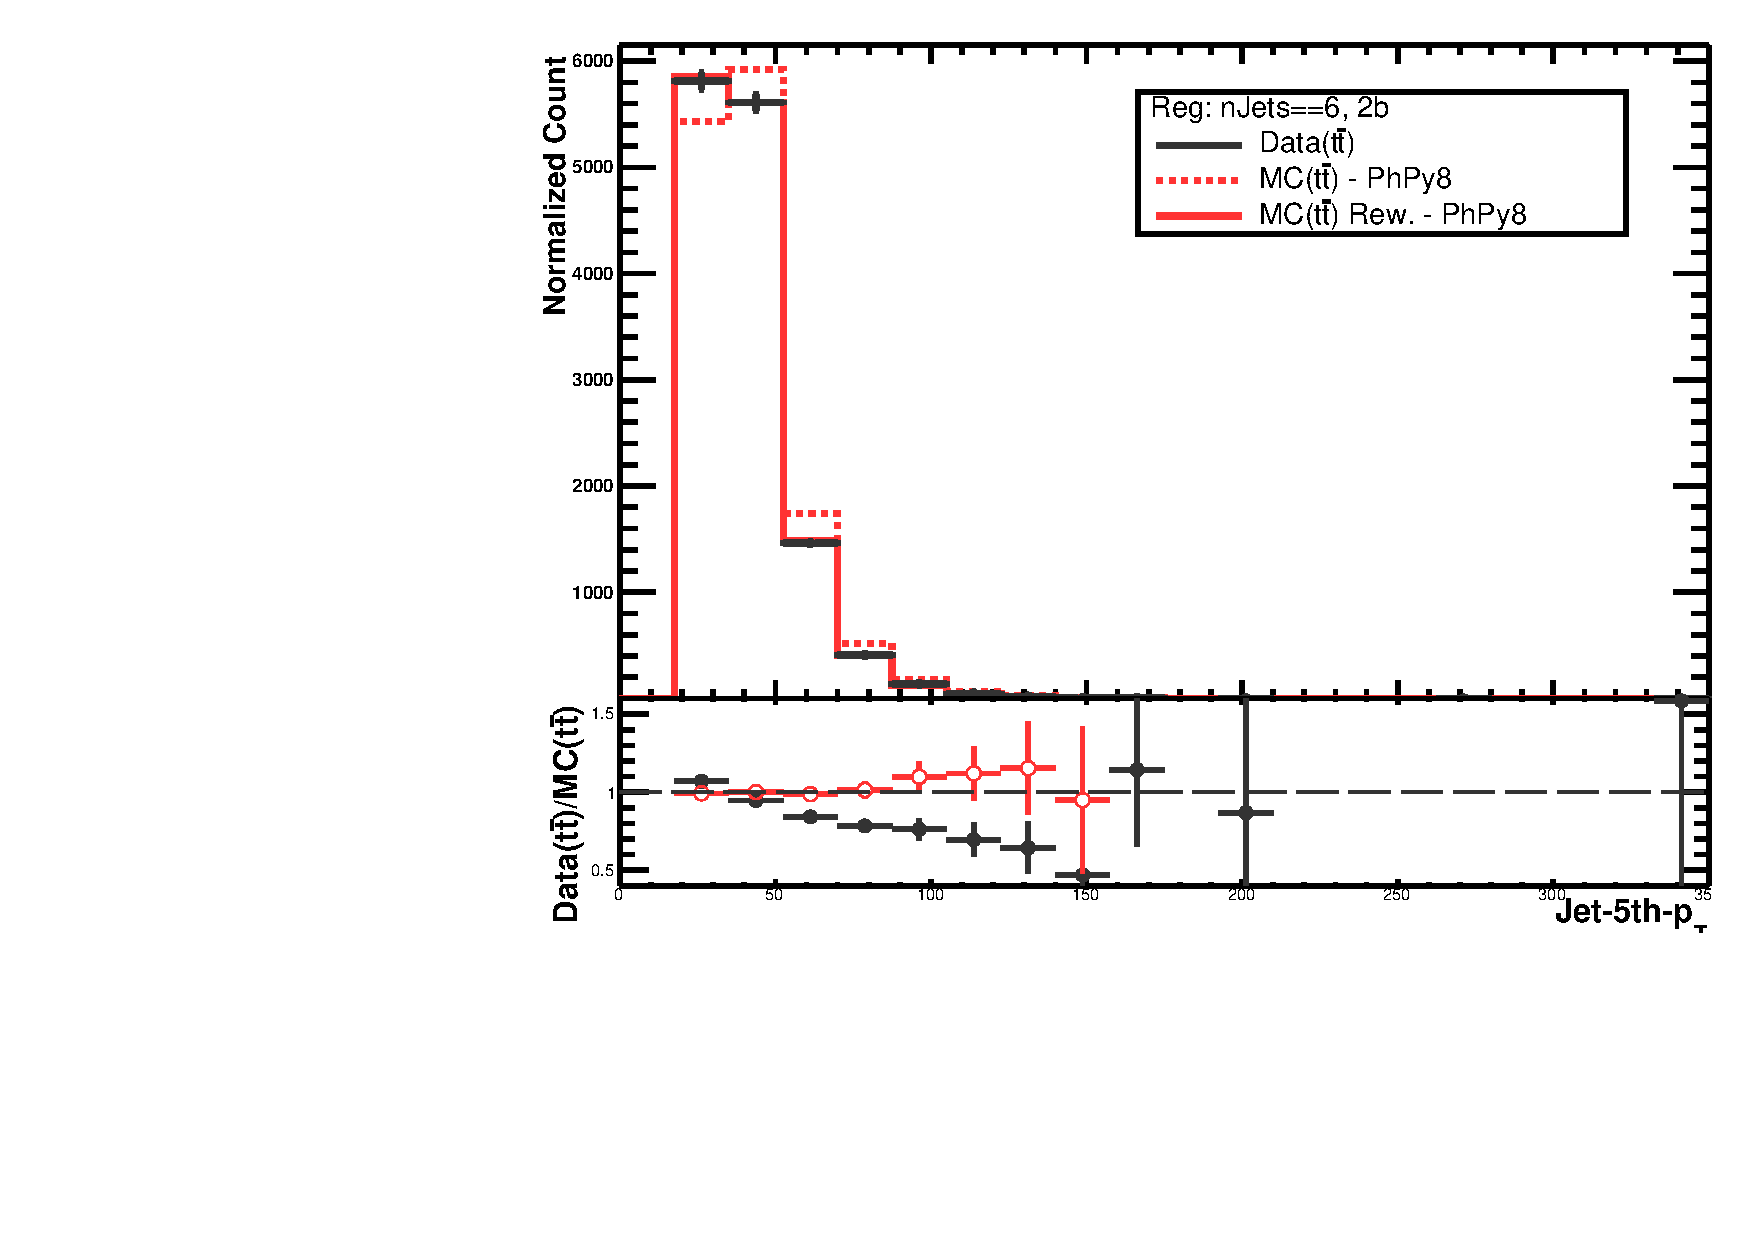
\includegraphics[width=0.24 \textwidth]{figures/rew_datamc_hfinckin_212169/1_ratiojet_pt_4__1e3_nJetsee6__2LOS.pdf} &
    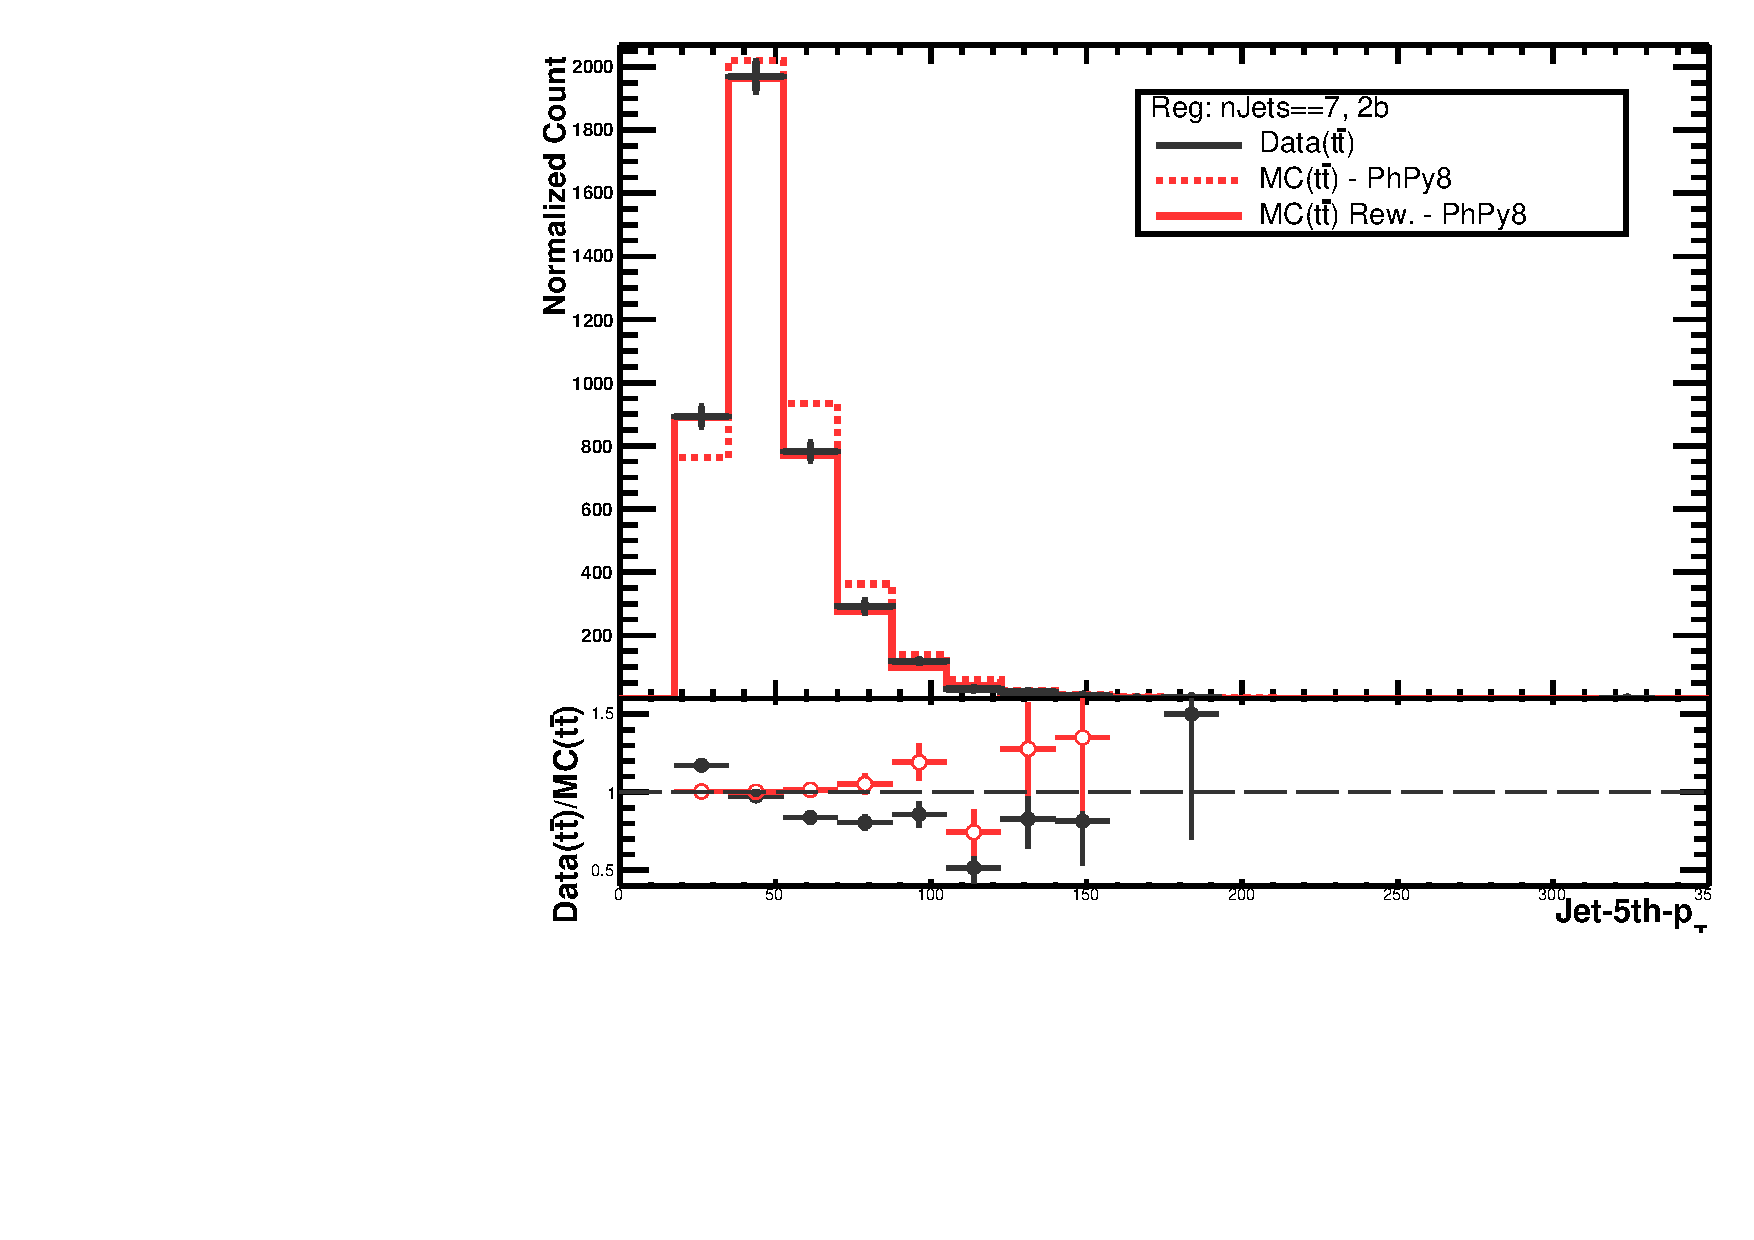
\includegraphics[width=0.24 \textwidth]{figures/rew_datamc_hfinckin_212169/1_ratiojet_pt_4__1e3_nJetsee7__2LOS.pdf} &
    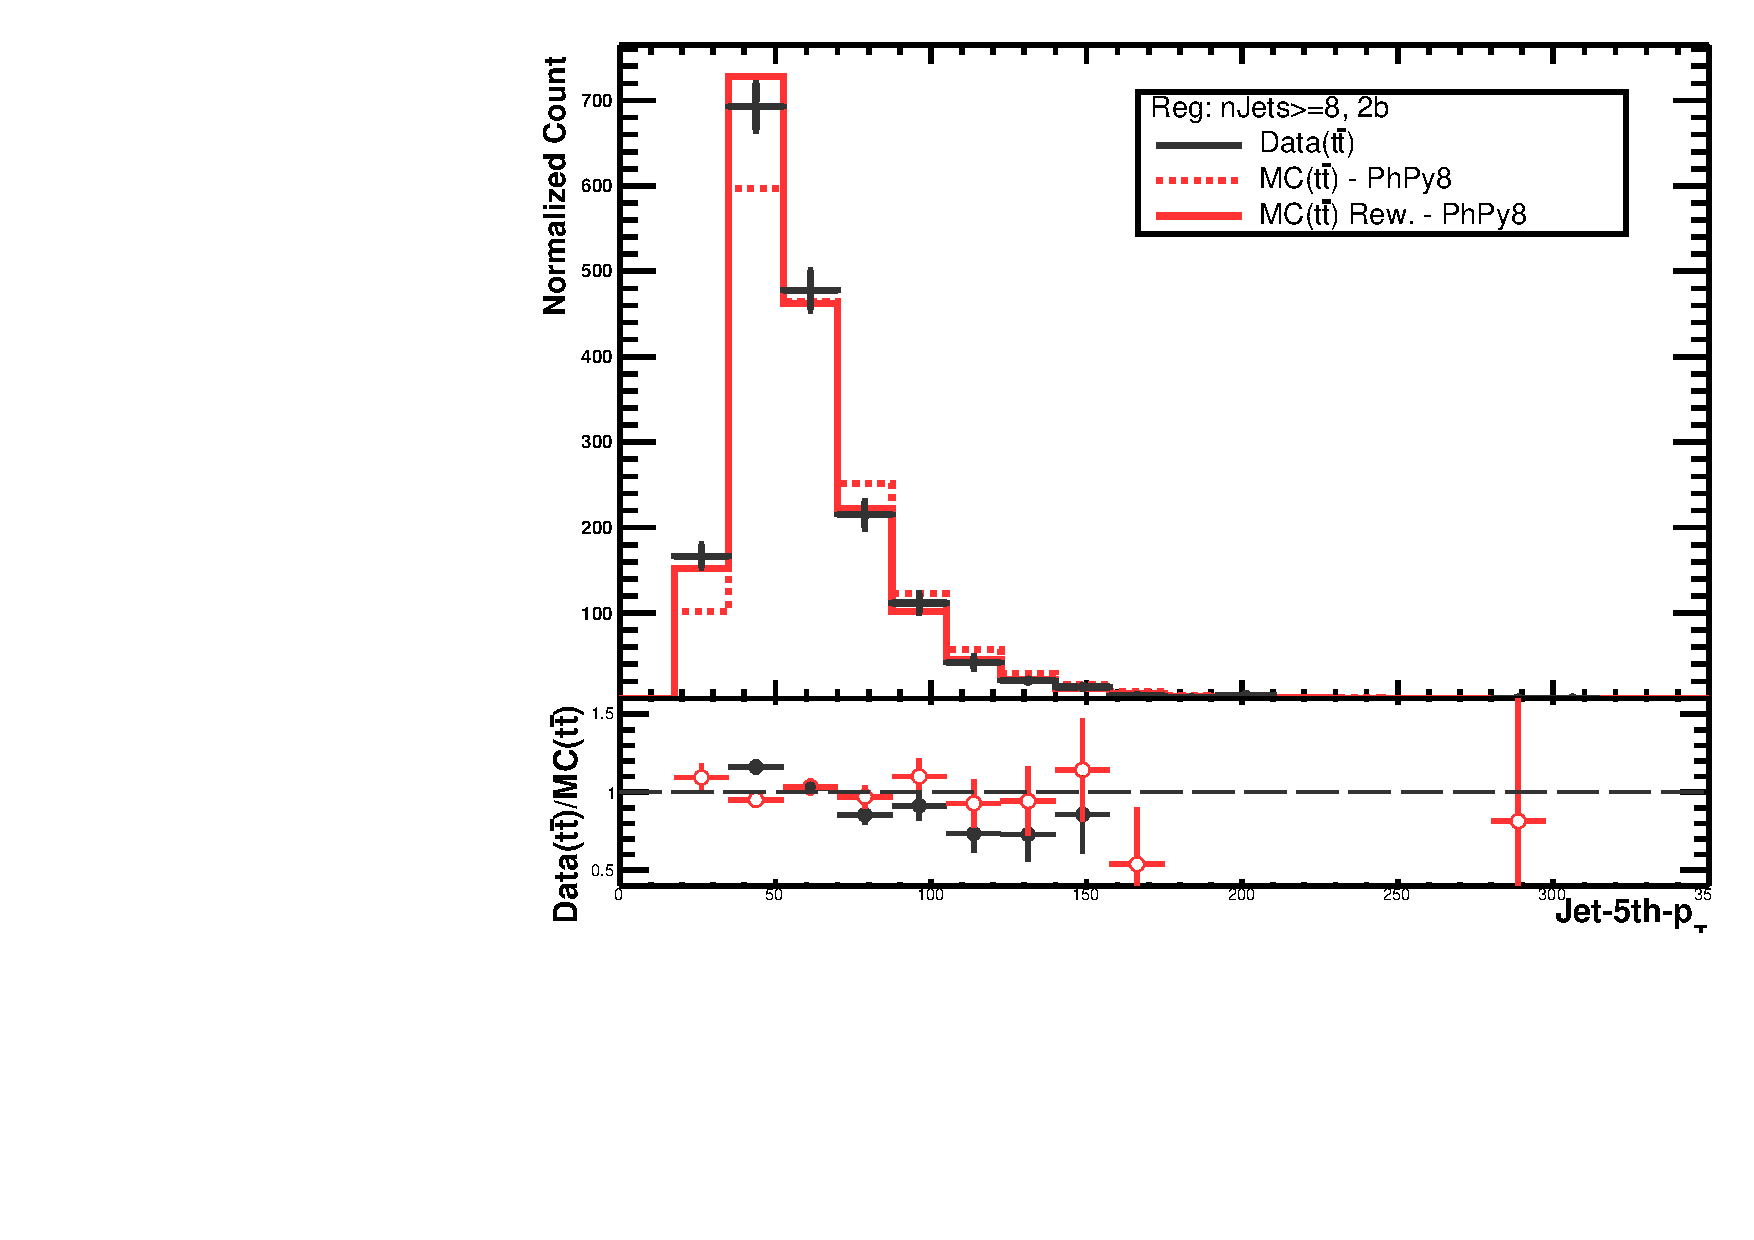
\includegraphics[width=0.24 \textwidth]{figures/rew_datamc_hfinckin_212169/1_ratiojet_pt_4__1e3_nJetsge8__2LOS.pdf} \\

    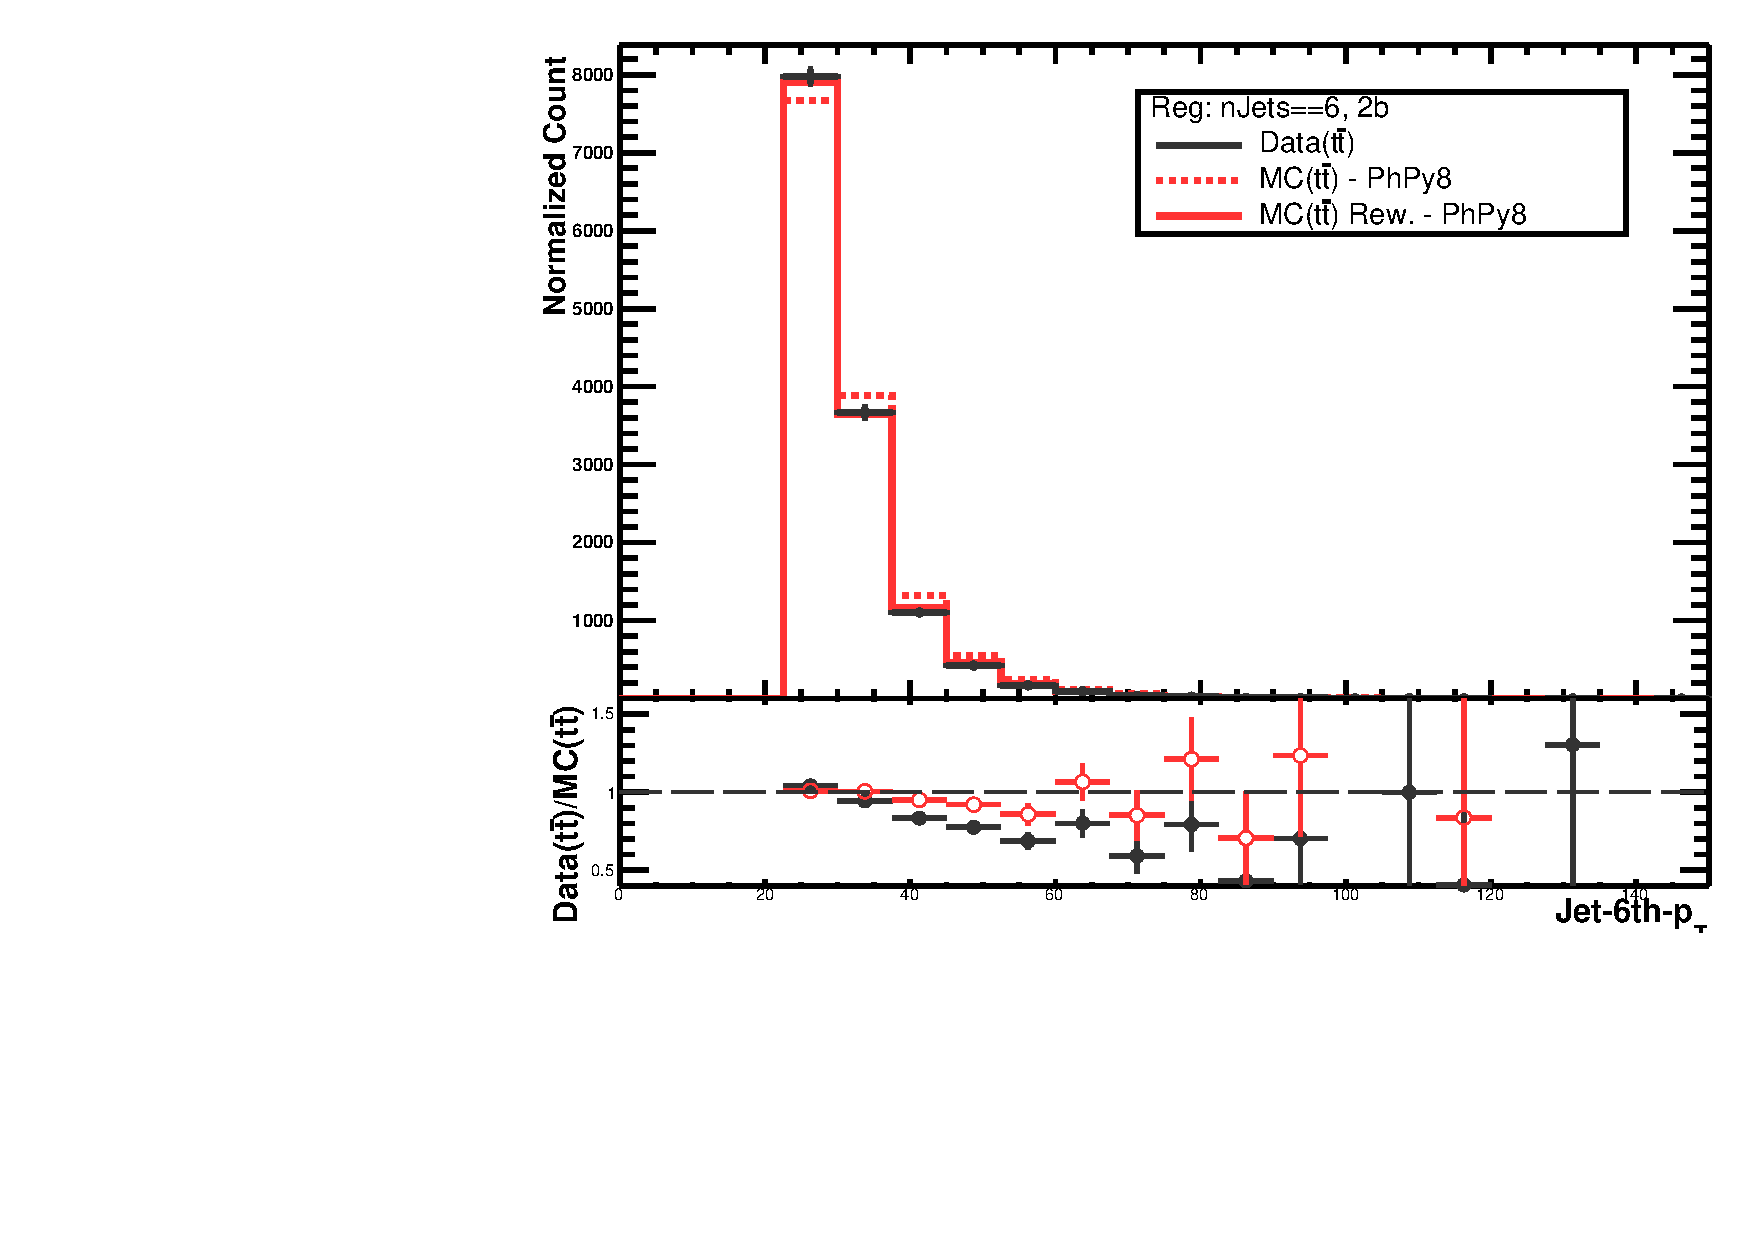
\includegraphics[width=0.24 \textwidth]{figures/rew_datamc_hfinckin_212169/1_ratioAlt__jet_pt_5__0__1e3_nJetsee6__2LOS.pdf} &
    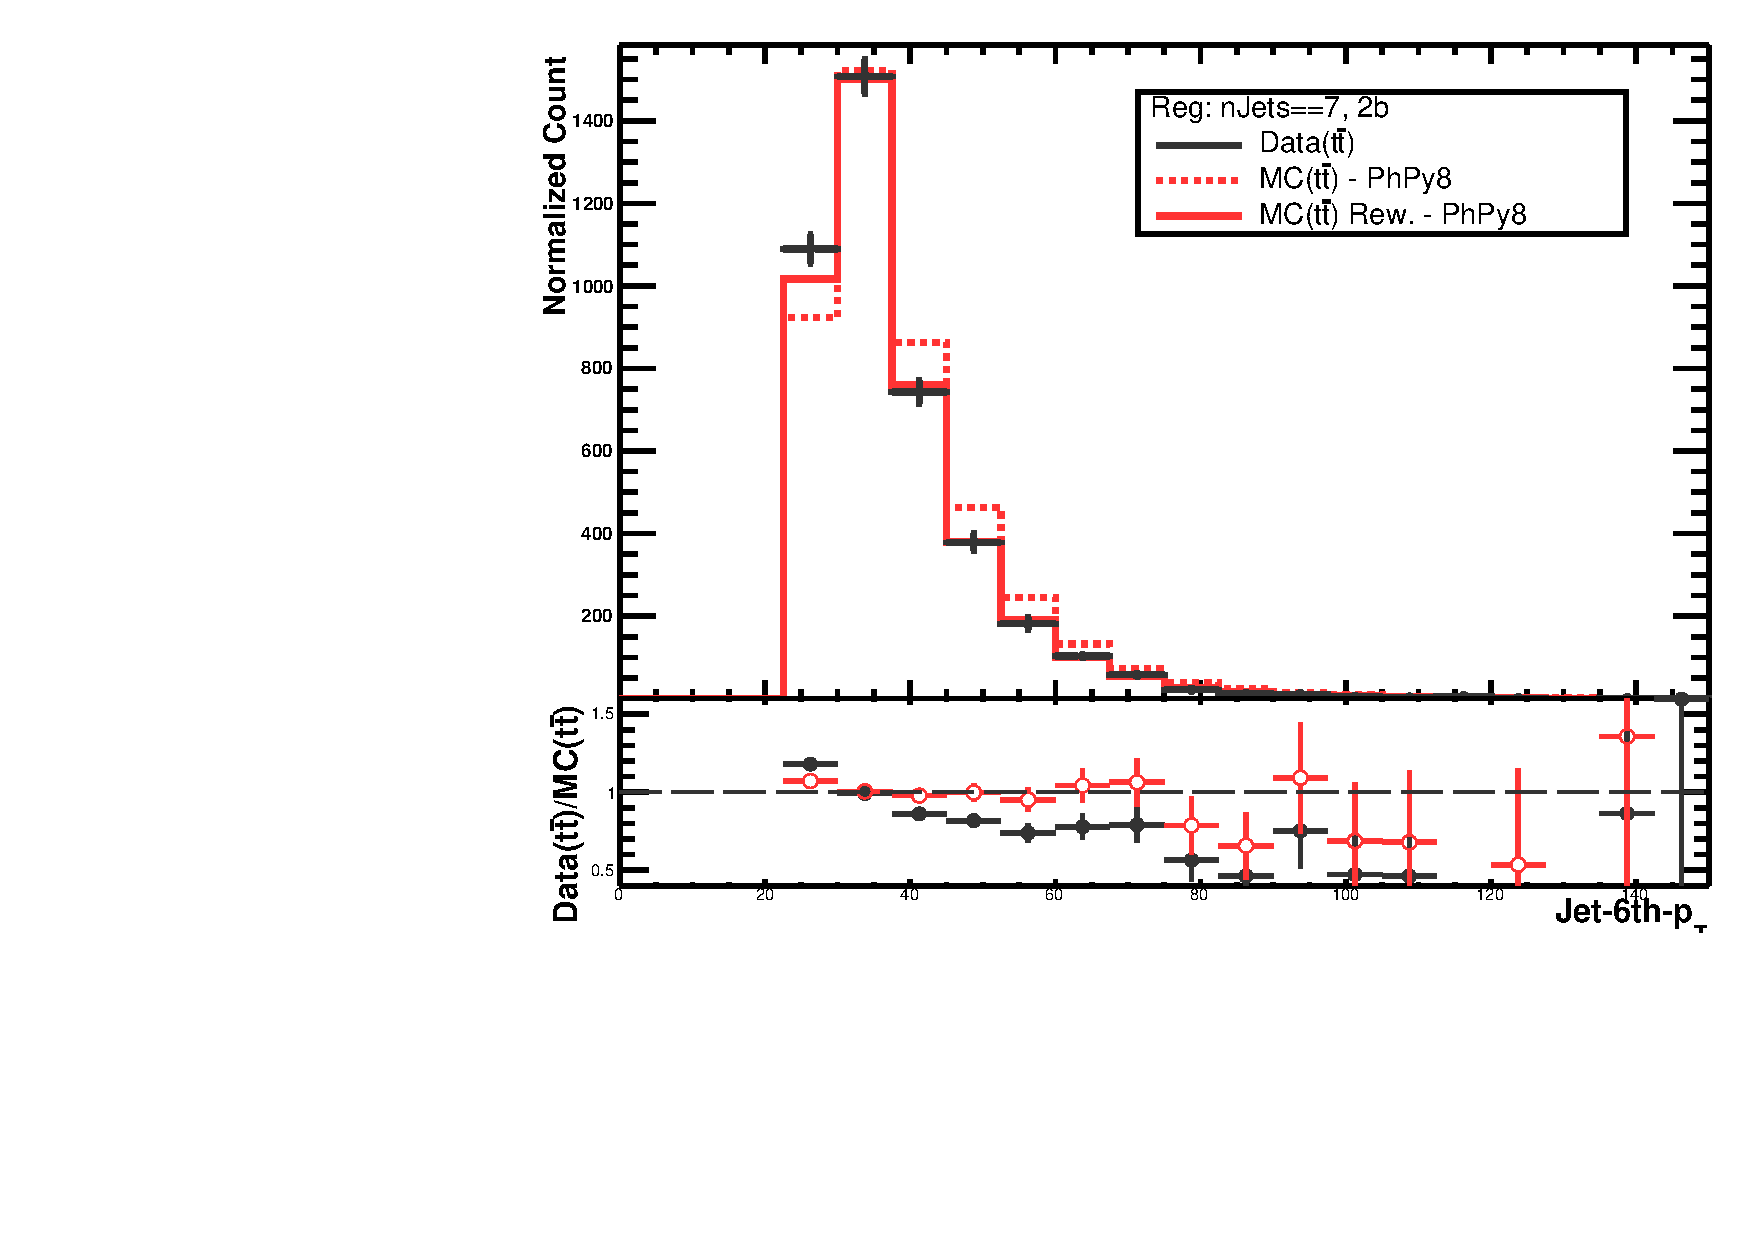
\includegraphics[width=0.24 \textwidth]{figures/rew_datamc_hfinckin_212169/1_ratioAlt__jet_pt_5__0__1e3_nJetsee7__2LOS.pdf} &
    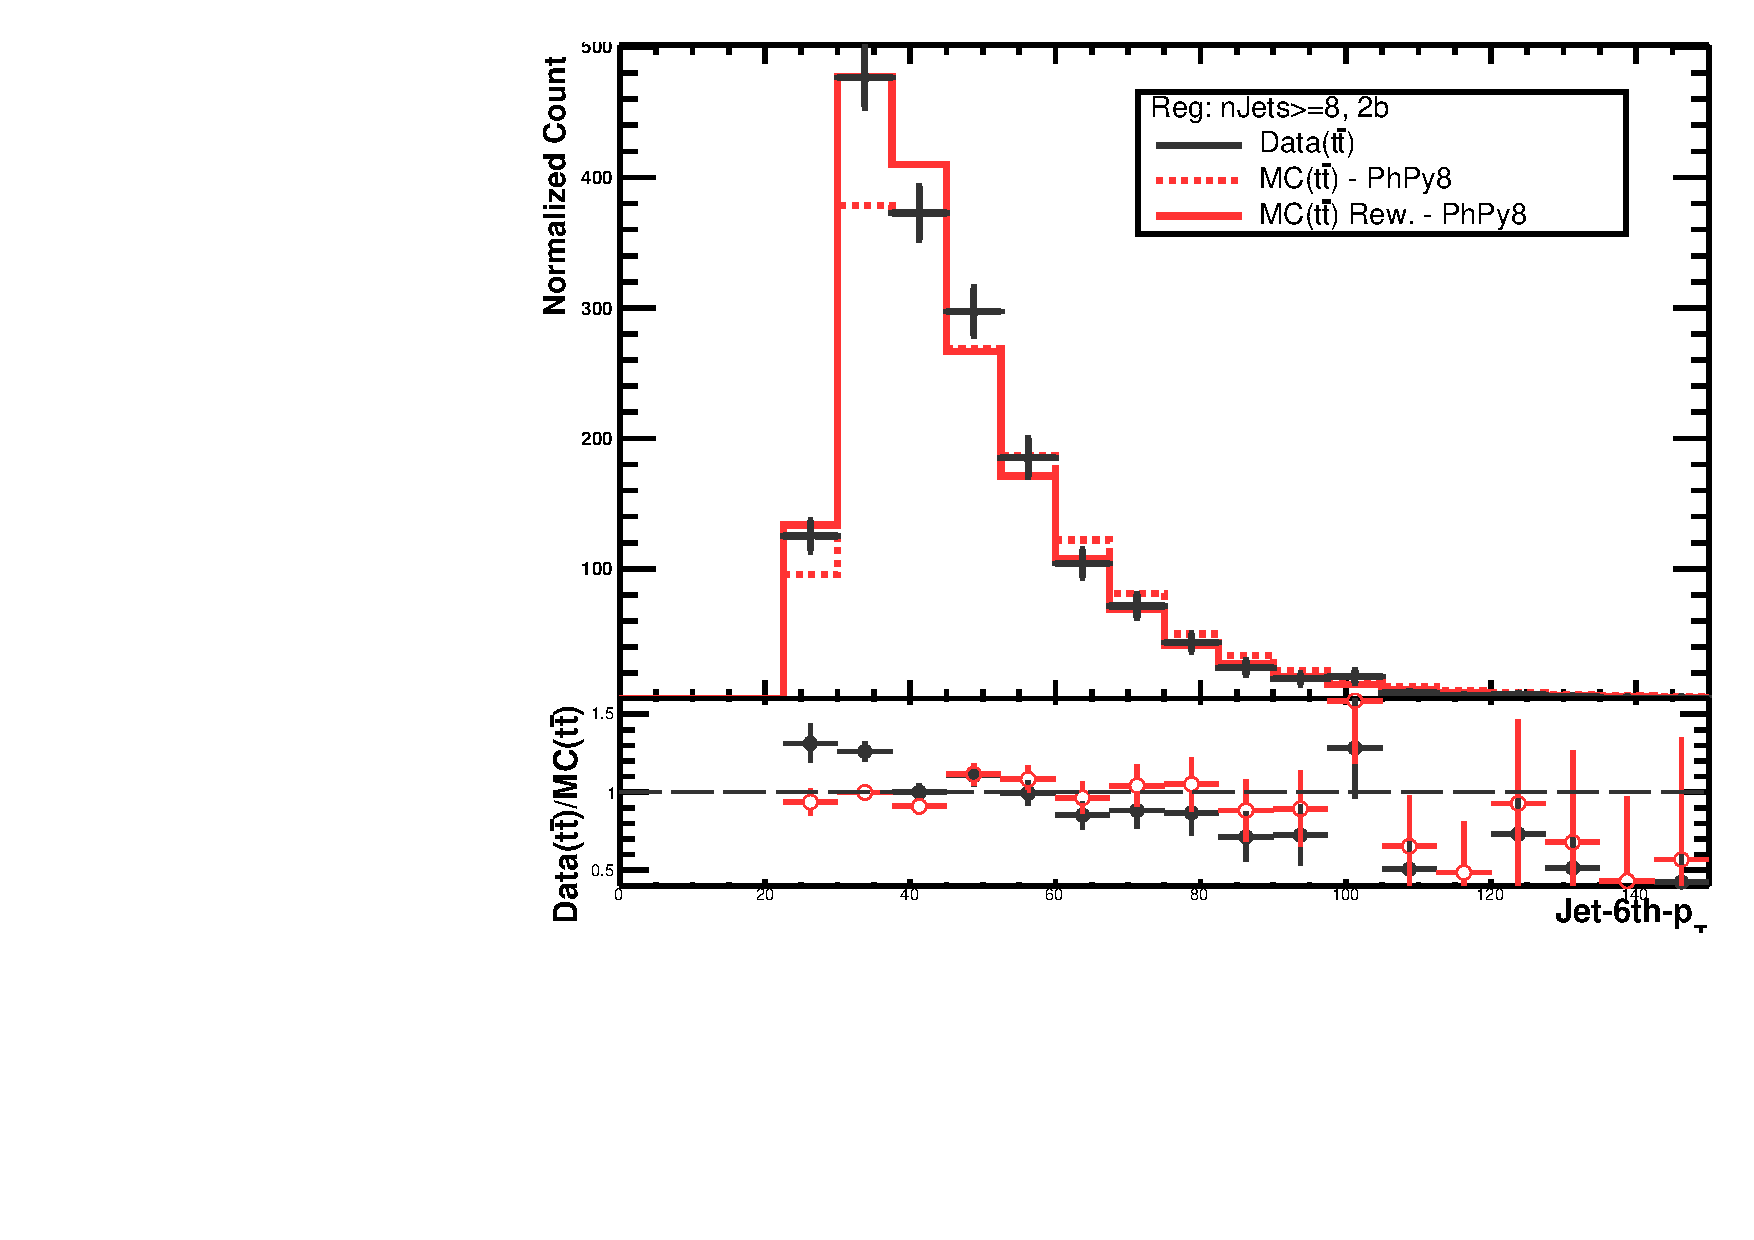
\includegraphics[width=0.24 \textwidth]{figures/rew_datamc_hfinckin_212169/1_ratioAlt__jet_pt_5__0__1e3_nJetsge8__2LOS.pdf} &
    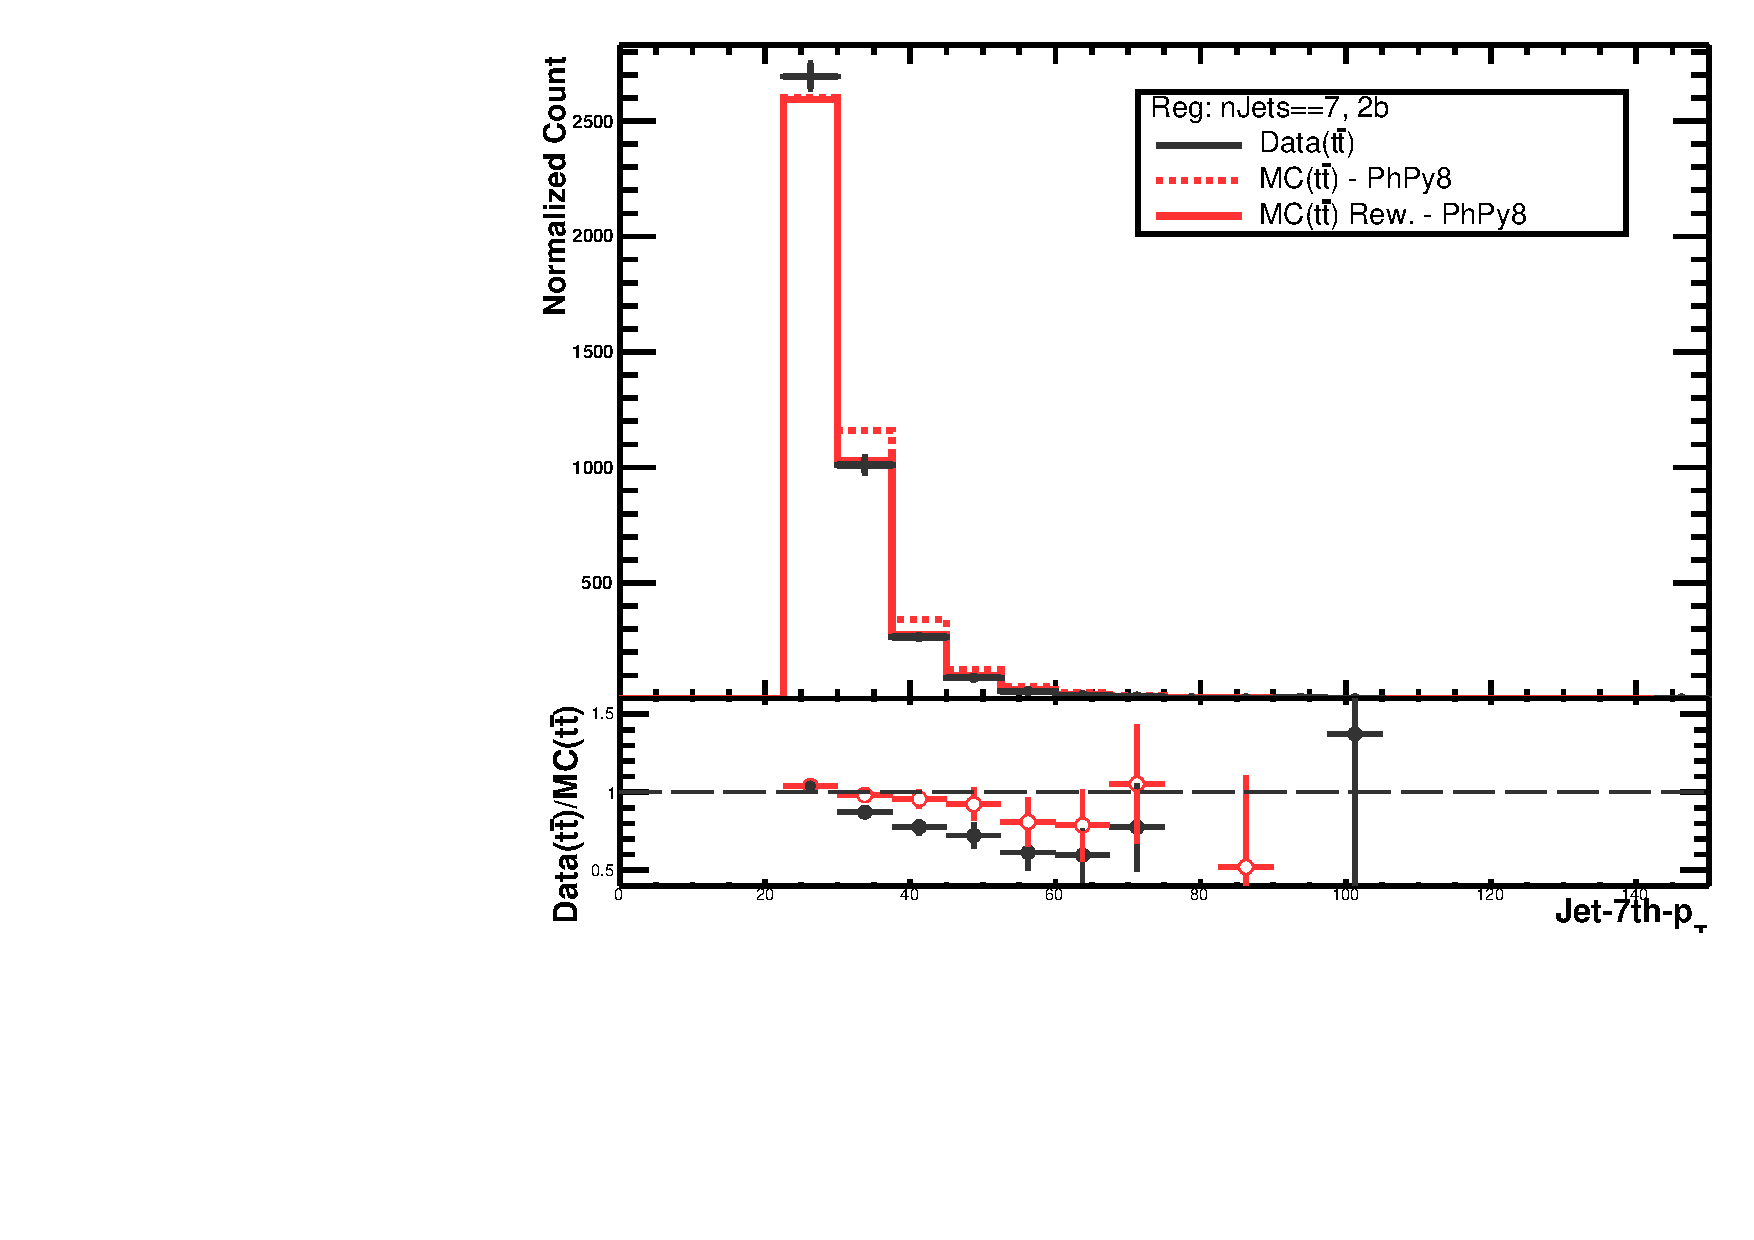
\includegraphics[width=0.24 \textwidth]{figures/rew_datamc_hfinckin_212169/1_ratioAlt__jet_pt_6__0__1e3_nJetsee7__2LOS.pdf} \\

    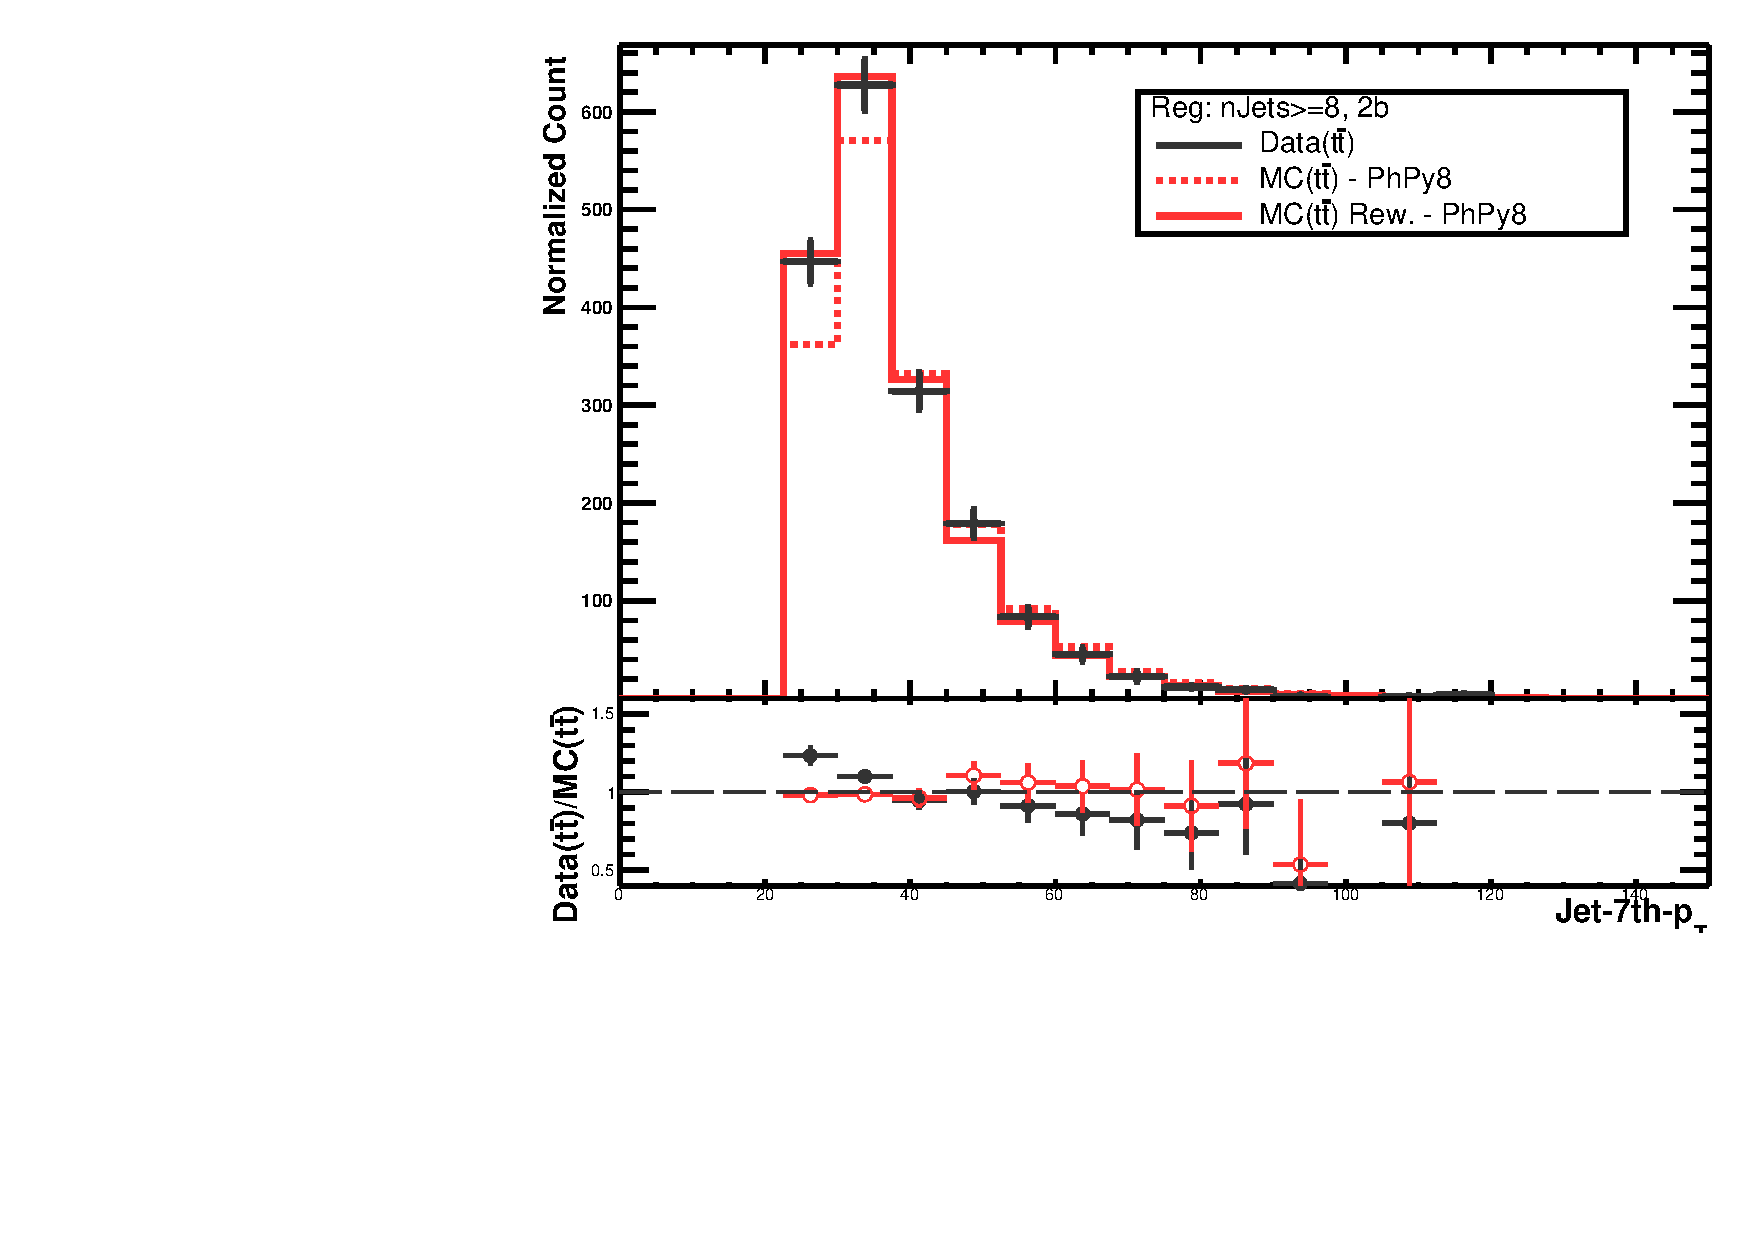
\includegraphics[width=0.24 \textwidth]{figures/rew_datamc_hfinckin_212169/1_ratioAlt__jet_pt_6__0__1e3_nJetsge8__2LOS.pdf} &
    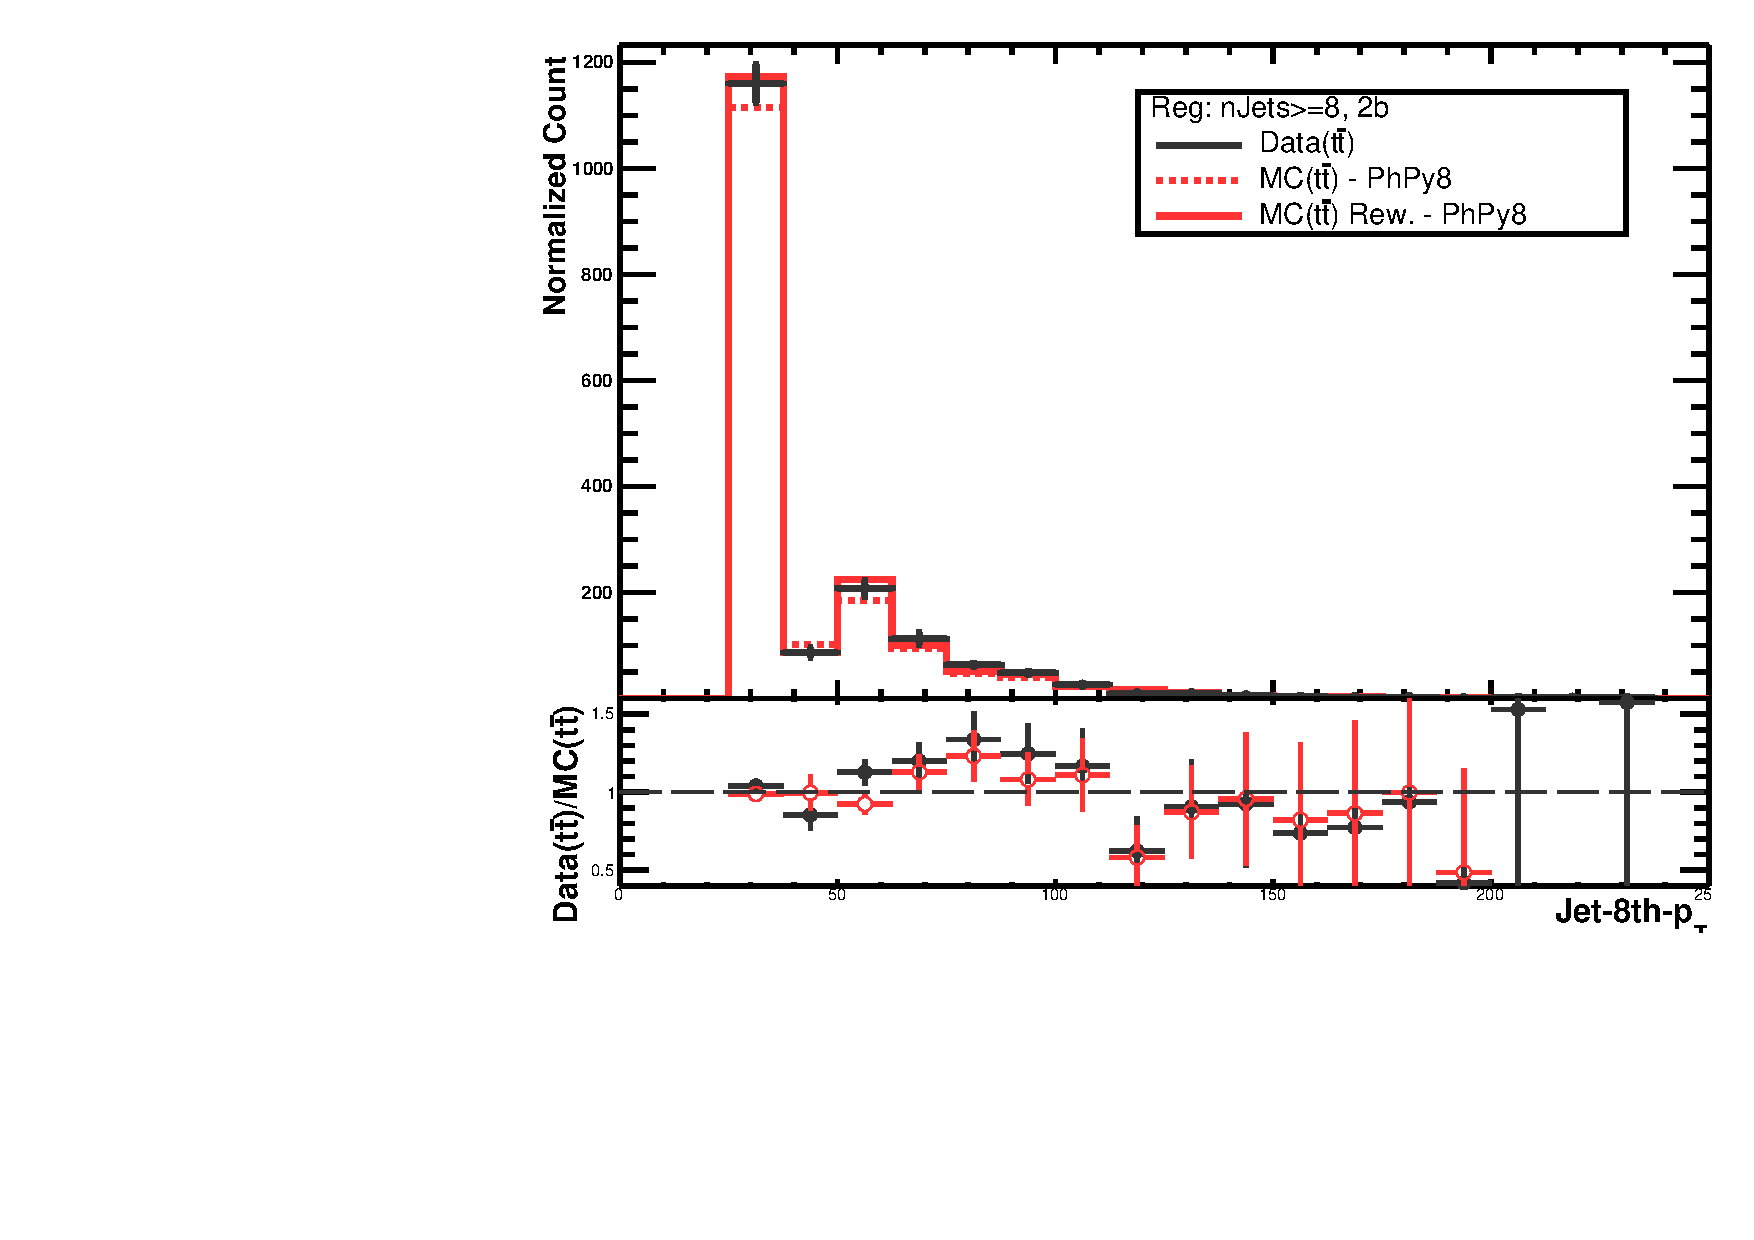
\includegraphics[width=0.24 \textwidth]{figures/rew_datamc_hfinckin_212169/1_ratioSum__jet_pt__Iteration_ge7___1e3_nJetsge8__2LOS.pdf} \\

    \end{tabular}
    \caption{\label{fig:recent_rew_2los} Some examples of NN reweighting for different features in 2LOS channel.}

\end{center}
\end{figure}